% =====================================================================
%  Improved Upper and Lower Bounds for Star-Shaped Kakeya Sets
%  Build:  tectonic -X compile star_shaped_kakeya_bounds.tex
%  Author: Ziyu Zhou.
% =====================================================================
\documentclass[11pt]{article}

\usepackage[margin=1.05in]{geometry}
\usepackage{amsmath,amssymb,amsthm}
\usepackage{mathtools}
\usepackage{array}
\usepackage{booktabs}
\usepackage{microtype}
\usepackage{tikz}
\usetikzlibrary{arrows.meta,calc,patterns,decorations.pathreplacing}
\usepackage{hyperref}
\usepackage{xurl}
\hypersetup{
  colorlinks=true,
  linkcolor=[rgb]{0.10,0.20,0.55},
  citecolor=[rgb]{0.10,0.20,0.55},
  urlcolor=[rgb]{0.10,0.30,0.45},
  pdftitle={Improved Upper and Lower Bounds for Star-Shaped Kakeya Sets},
  pdfauthor={Ziyu Zhou}
}

% ---------------------------------------------------------------- theorems
\theoremstyle{plain}
\newtheorem{theorem}{Theorem}[section]
\newtheorem{proposition}[theorem]{Proposition}
\newtheorem{lemma}[theorem]{Lemma}
\newtheorem{corollary}[theorem]{Corollary}
\newtheorem{maintheorem}{Theorem}
\renewcommand{\themaintheorem}{\Alph{maintheorem}}

\theoremstyle{definition}
\newtheorem{definition}[theorem]{Definition}
\newtheorem{convention}[theorem]{Convention}

\theoremstyle{remark}
\newtheorem{remark}[theorem]{Remark}

% ---------------------------------------------------------------- macros
\newcommand{\R}{\mathbb{R}}
\newcommand{\Q}{\mathbb{Q}}
\newcommand{\Z}{\mathbb{Z}}
\newcommand{\Tp}{\mathbb{T}_{\pi}}
\newcommand{\Lout}{\mathcal{L}^{*}_{2}}
\newcommand{\Lone}{\mathcal{L}^{*}_{1}}
\newcommand{\Astar}{A_{*}}
\newcommand{\Aturn}{A_{*}^{\mathrm{turn}}}
\newcommand{\conv}{\operatorname{conv}}
\newcommand{\Rsta}{R_{\mathrm{s}}}
\newcommand{\Rend}{R_{\mathrm{e}}}
\newcommand{\Ps}{P_{\mathrm{s}}}
\newcommand{\Pe}{P_{\mathrm{e}}}
\newcommand{\Ain}{A_{\mathrm{in}}}
\newcommand{\Aout}{A_{\mathrm{out}}}
\newcommand{\Istar}{I_{*}}
\newcommand{\Hsup}{H_{\mathrm{sup}}}
\newcommand{\epsdel}{\varepsilon_{\mathrm{del}}}
\newcommand{\Tri}{\mathcal{T}}
% \lean typesets identifiers in typewriter face and allows line breaks
% after the underscores and dots of long Lean names.
\newcommand{\lean}[1]{%
  \begingroup\ttfamily\hyphenchar\font=-1\relax
  \def\_{\textunderscore\allowbreak}%
  #1\endgroup}

\allowdisplaybreaks

\title{Improved Upper and Lower Bounds\\ for Star-Shaped Kakeya Sets}
\author{Ziyu Zhou}
\date{2 August 2026}

\begin{document}
\maketitle

\begin{abstract}
A planar star-shaped Kakeya set is star-shaped about some point and contains a
closed unit segment in every unoriented direction. Let $\Astar$ denote the
infimum of the two-dimensional Lebesgue \emph{outer} measure over this class; no
measurability and no continuous motion is assumed. We prove
\[
  \frac{131\pi}{6250}\ \le\ \Astar\ <\ \frac{77\pi}{851}.
\]
The lower estimate is obtained for every individual set: each star-shaped
Kakeya set has outer measure strictly larger than $131\pi/6250$. Its proof
refines the circular-section method used by Cunningham and by Li; the main
ingredients are a same-centre dilation estimate for arbitrary families of arcs
on the projective circle, an endpoint-containment argument formulated on the
oriented-to-projective quotient, a polar slicing step for outer measure, and an
additive mechanism in which a measurable closed ball separates two payments:
directions whose triangle stays in a fixed disk are charged only inside the
ball, directions that escape it are charged only outside, and the two charges
are added by Carath\'eodory splitting instead of being compared in a minimax.
The exterior charge rests on the observation that a unit segment avoiding a
disk casts a one-sided, rather than symmetric, angular shadow. A baseline
route with the weaker constant $100\pi/5599$, proved by a three-branch
fixed-parameter estimate, is retained in full.
For the upper estimate we exhibit one explicit compact set: it is star-shaped,
it admits a continuous endpoint-reversing half-turn of a unit segment, it is
built from $100001$ congruent cells generated by two rational polynomial
profiles, and its area is strictly below the classical
Cunningham--Schoenberg value $(5-2\sqrt2)\pi/24$. Its area is controlled by a
two-branch limiting radial envelope whose five branch switches are isolated
exactly, by a six-piece polynomial antiderivative identity, and by a
quantitative finite-cell lift. Lean~4 developments over a pinned Mathlib
revision verify the mathematical assembly of both displayed inequalities; the
upper development additionally checks generated algebraic certificates by scoped
native evaluation, which we describe precisely. The two bounds do not determine
$\Astar$, and we claim no optimality.
\end{abstract}

\tableofcontents

% =====================================================================
\section{Introduction}\label{sec:intro}

\subsection{The problem}

The Kakeya needle problem asks how small a planar region can be if a unit
segment can be turned continuously inside it through a half-turn. Besicovitch
showed that, after the standard reduction from the needle-rotation formulation
to the containment formulation, the unrestricted problem admits sets of
arbitrarily small area \cite{Besicovitch1928}. A geometric side condition
changes the picture completely. If a set is star-shaped about a point $O$, then
every unit segment $\ell\subset E$ drags with it the filled triangle
$\conv(\{O\}\cup\ell)$, whose area is half the distance from $O$ to the line of
$\ell$. Positive lower bounds then become possible, and the extremal problem
acquires a finite positive answer.

Throughout, a set $E\subset\R^{2}$ is a \emph{star-shaped Kakeya set} if it is
star-shaped about some point and contains a closed unit segment in every
unoriented direction; see Section~\ref{sec:defs} for the precise definitions,
including the outer-measure conventions used for possibly nonmeasurable sets.
We write
\[
  \Astar:=\inf\bigl\{\Lout(E)\ :\ E\subset\R^{2}
  \text{ is a star-shaped Kakeya set}\bigr\}.
\]

\subsection{Known bounds}

The following four results delimit what was known.

\begin{itemize}
  \item Besicovitch \cite{Besicovitch1928}: without a shape restriction the
    infimum is $0$.
  \item Cunningham and Schoenberg \cite{CunninghamSchoenberg1965} studied the
    Kakeya constant for simply connected sets admitting a continuous turning
    motion and produced a sequence of star-shaped domains whose areas approach
    \[
      \frac{(5-2\sqrt2)\pi}{24}=0.28425\ldots
    \]
    Their paper records that Melvin Bloom had obtained the same estimate earlier
    by the same construction; we preserve this attribution whenever the 1965
    value is discussed historically.
  \item Cunningham \cite{Cunningham1971} treated the star-shaped problem
    explicitly and proved the lower bound $\pi/108$.
  \item Li \cite{Li2026} worked with arbitrary, possibly nonmeasurable
    star-shaped Kakeya sets and proved $\Lout(E)\ge\pi/98$ by a circular-section
    argument with an interior/exterior decomposition of the direction circle.
    (The journal version appeared in 2026; the preprint was first posted in
    2025.)
\end{itemize}

To the best of our knowledge these are the strongest published bounds for their
respective classes; we make no claim of historical priority.

\subsection{The main theorem}

\begin{maintheorem}\label{thm:A}
Let $\Astar$ be the infimum of the planar Lebesgue outer measure over all
star-shaped Kakeya sets. Then
\[
  \boxed{\ \frac{131\pi}{6250}\ \le\ \Astar\ <\ \frac{77\pi}{851}.\ }
\]
More precisely:
\begin{enumerate}
  \item[\textup{(i)}] every star-shaped Kakeya set $E\subset\R^{2}$, with no
    measurability assumption whatsoever, satisfies
    \[
      \Lout(E)>\frac{131\pi}{6250};
    \]
  \item[\textup{(ii)}] the explicit compact set $E_{100001}\subset\R^{2}$ of
    Sections~\ref{sec:construction} and~\ref{sec:finitelift} is star-shaped
    about the origin, carries a continuous endpoint-reversing half-turn of a
    unit segment, and satisfies
    \[
      |E_{100001}|<\frac{77\pi}{851}<\frac{(5-2\sqrt2)\pi}{24}.
    \]
\end{enumerate}
\end{maintheorem}

Numerically, and strictly secondarily to the exact statement,
\[
  \frac{131}{6250}=0.02096,\qquad
  \frac{77}{851}=0.0904817\ldots,\qquad
  \frac{5-2\sqrt2}{24}=0.0904822\ldots
\]
after normalisation by $\pi$; the ratio between the two endpoints of
Theorem~\ref{thm:A} is $481250/111481=4.3168\ldots$, so the problem remains
widely open. The lower endpoint is proved twice, by two routes with different
parameters and different exterior geometry: a baseline route
(Sections~\ref{sec:trichotomy}--\ref{sec:caseII}), which gives the weaker
constant $100\pi/5599$ and is retained in full, and the additive refinement of
Sections~\ref{sec:additive} and~\ref{sec:annbudget}, which gives the displayed
constant and improves the baseline one by the factor
$733469/625000=1.1735\ldots$, that is by $17.36\%$.

\begin{remark}[strict versus non-strict inequalities]\label{rem:strict}
Statement (i) is strict for each individual set, but an infimum of numbers each
strictly larger than a constant need only be $\ge$ that constant. Hence (i)
yields exactly $\Astar\ge131\pi/6250$, and \emph{not}
$\Astar>131\pi/6250$: nothing in our argument produces a uniform gap above
$131\pi/6250$. By contrast the upper inequality of Theorem~\ref{thm:A}
\emph{is} strict at the displayed constant, because the infimum is bounded above
by the area of one particular admissible set, and that area is strictly below
$77\pi/851$.
\end{remark}

\begin{corollary}\label{cor:historical}
The lower endpoint of Theorem~\ref{thm:A} improves the published general lower
bound $\pi/98$ of \cite{Li2026} by the factor $6419/3125=2.0540\ldots$, and the
explicit set $E_{100001}$ has area strictly smaller than the classical
Cunningham--Schoenberg value $(5-2\sqrt2)\pi/24$ of
\cite{CunninghamSchoenberg1965}.
\end{corollary}

\subsection{Strategy of the proof}\label{sec:strategy}

The two inequalities of Theorem~\ref{thm:A} are proved by independent arguments
with different data, and they meet only in the final infimum step. The lower
inequality is a statement about \emph{every} set in a very broad class: no
measurability of the set is assumed, and no measurability or continuity
assumption is made on the pointwise choice of needles. The upper inequality is a
statement about \emph{one} set in the strictly smaller continuous-turning
class.
Both arguments start from the same elementary observation
(Lemma~\ref{lem:triangle}): a needle inside a star-shaped set forces a filled
triangle with apex at the star centre, whose area is half the distance from the
centre to the needle's line.

For the upper bound, the triangle family is \emph{designed}. A unit segment is
carried around a half-turn by $n$ congruent cells; inside one cell the segment
slides tangentially by $a(t)$ and is pushed normally by $\pi s(t)/n$. Choosing
$n$ odd makes the ordered endpoints exchange after the turn, which is what the
turning definition requires. The two profiles $a,s$ are the design variables;
they are constrained by cell joining, by reflection symmetry, and by a package
of sign conditions which force the limiting radial envelope of the swept union
to be the maximum of exactly two explicit branches. For an explicit rational
profile pair, five branch switches are isolated by exact algebraic elimination,
the resulting six-piece integral is evaluated by polynomial antiderivatives, and
a uniform $O(n^{-2})$ estimate transfers the limiting area bound to the literal
finite union.

For the lower bound, the triangle family is \emph{arbitrary}. One first asks
whether some triangle is high; if not, every triangle height is below a fixed
threshold, and the direction circle splits into the directions whose triangle
stays inside a fixed disk and those whose triangle escapes it. Confined
directions produce circular sections whose angular masses can be compared
through a same-centre dilation on the projective circle and then integrated
radially by polar slicing; escaping directions produce needles bounded away from
the star centre, whose triangles can be selected greedily, with a deletion
radius set by a fixed rule from the height of the selected triangle, so that the
deleted direction mass is paid for by disjoint triangle area.

How the two direction classes are combined is what separates the two lower
routes. The baseline route of
Sections~\ref{sec:trichotomy}--\ref{sec:caseII} lets them compete: a
proportion of the total direction mass is fixed in advance, each class charges
the whole set, and the proved constant is the value of a minimax. The
refinement of Sections~\ref{sec:additive} and~\ref{sec:annbudget} lets them
cooperate: a measurable closed ball splits the \emph{plane}, the confined class
is charged only inside it and the escaping class only outside it, so that
Carath\'eodory splitting adds the two charges exactly, even though the set is
not assumed measurable. Adding rather than comparing costs the escaping class a
sharper estimate, which comes from the fact that a unit segment avoiding a disk
cannot straddle it and therefore casts a one-sided angular shadow. Each branch
of each route is closed by exact rational arithmetic at one fixed parameter
tuple.

Section~\ref{sec:pipelines} sets out both pipelines in full before any technical
formula is introduced.

\subsection{Formal verification}

Both displayed inequalities of Theorem~\ref{thm:A} are supported by Lean~4
developments over a single pinned Mathlib revision, together with independent
exact-arithmetic certificate generators. The two halves do not carry the same
trust: both lower theorems --- the baseline one and the refinement --- use only
the three standard Mathlib axioms, whereas the upper theorem additionally
depends on reflection axioms generated by scoped \lean{native\_decide}
evaluation of large decidable algebraic checks.
Appendix~\ref{app:formalization} makes this precise and states the evidence
boundary; Appendix~\ref{app:repro} gives the reproduction commands. A successful
build is evidence about a formal artefact, not a substitute for mathematical
refereeing, and it implies nothing about optimality or priority.

\subsection{Organisation}

Section~\ref{sec:defs} fixes definitions, measure conventions, the two
admissible classes, the common triangle reduction, both proof pipelines and the
notation. Part~\ref{part:upper}
(Sections~\ref{sec:construction}--\ref{sec:finitelift}) designs the profiles,
analyses the limiting envelope and performs the finite-cell lift.
Part~\ref{part:lower} (Sections~\ref{sec:trichotomy}--\ref{sec:caseII}) proves
the baseline universal lower bound $100\pi/5599$ through the radius trichotomy,
the confined-direction branch and the escaping-direction branch;
Sections~\ref{sec:additive} and~\ref{sec:annbudget} then prove the additive
confined/exterior refinement, which yields the displayed constant
$131\pi/6250$. Section~\ref{sec:assembly} assembles
Theorem~\ref{thm:A} and Section~\ref{sec:discussion} states the open problems.
Appendix~\ref{app:constants} collects the exact certificate constants,
Appendix~\ref{app:formalization} the formalisation architecture and trusted
computing base, and Appendix~\ref{app:repro} the reproduction commands.

% =====================================================================
\section{Definitions, common geometry and the two pipelines}\label{sec:defs}

\subsection{Directions, needles and star-shapedness}

We work in $\R^{2}$ with its Euclidean structure. For $\theta\in\R$ put
\[
  e(\theta)=(\cos\theta,\sin\theta).
\]
Unoriented directions form the quotient circle
\begin{equation}\label{eq:projcircle}
  \Tp:=\R/\pi\Z ,
\end{equation}
equipped with its quotient metric and with the Haar measure of total mass $\pi$;
we call the latter \emph{direction mass}. The canonical map
$\R/2\pi\Z\to\Tp$ from oriented angles to unoriented directions is two-to-one,
and keeping track of it is essential in Section~\ref{sec:caseI}.

\begin{definition}[star-shaped set]
A set $E\subset\R^{2}$ is \emph{star-shaped about} $O\in\R^{2}$ if
$[O,x]\subset E$ for every $x\in E$, where $[O,x]$ denotes the closed segment.
No convexity, closedness or measurability is assumed.
\end{definition}

\begin{definition}[star-shaped Kakeya set]\label{def:ssk}
A set $E\subset\R^{2}$ is a \emph{star-shaped Kakeya set} if there exists
$O\in\R^{2}$ such that $E$ is star-shaped about $O$ and, for every
$\alpha\in\Tp$, the set $E$ contains a closed unit segment whose direction is
$\alpha$. We call $O$ a \emph{star centre} and any such segment a \emph{needle}
in direction $\alpha$.
\end{definition}

\begin{convention}[outer measures]\label{conv:outer}
Since Definition~\ref{def:ssk} imposes no measurability, all sizes below are
outer measures:
\begin{itemize}
  \item $\Lout$ denotes planar Lebesgue outer measure; it agrees with area on
    measurable sets, and for the explicit set of Part~\ref{part:upper} we write
    $|\cdot|$ because that set is compact;
  \item $\Lone$ denotes one-dimensional outer measure on $\Tp$ normalised so
    that $\Lone(\Tp)=\pi$;
  \item circular sections are measured with one-dimensional Hausdorff outer
    measure, transported to angular outer measure by the arclength
    parametrisation of a circle of radius $r$.
\end{itemize}
All computations with these quantities take place in $[0,\infty]$; in the
formalisation the value $+\infty$ is carried explicitly rather than being
excluded by hypothesis.
\end{convention}

\begin{definition}[the constant]\label{def:Astar}
\[
  \Astar:=\inf\bigl\{\Lout(E):E\subset\R^{2}\text{ is a star-shaped Kakeya set}
  \bigr\}.
\]
\end{definition}

The infimum is over a nonempty class (a disk of radius $1$ qualifies), so
$0\le\Astar<\infty$.

\subsection{The continuous-turning subclass}

The set constructed in Part~\ref{part:upper} satisfies a strictly stronger
condition, and we keep the two classes apart.

\begin{definition}[turning needle]\label{def:turning}
A \emph{continuous turning needle} in $E\subset\R^{2}$ is a pair of continuous
maps $p,q:[0,\pi]\to\R^{2}$ with
\[
  q(\theta)-p(\theta)=e(\theta),\qquad
  [p(\theta),q(\theta)]\subset E\qquad(0\le\theta\le\pi),
\]
and with the endpoint reversal
\[
  p(\pi)=q(0),\qquad q(\pi)=p(0).
\]
\end{definition}

\begin{definition}[admissible set]\label{def:admissible}
A set $E\subset\R^{2}$ is \emph{admissible} if it is bounded, Lebesgue
measurable, star-shaped about some point, and carries a continuous turning
needle. Write
\[
  \Aturn:=\inf\{|E|:E\text{ admissible}\}.
\]
\end{definition}

The oriented equation $q(\theta)-p(\theta)=e(\theta)$ prescribes every
intermediate direction, and the reversal condition forbids a direction-by-direction
selection that jumps to unrelated endpoints at the end of the motion. Every
admissible set is in particular a star-shaped Kakeya set, so
\begin{equation}\label{eq:classes}
  \Astar\ \le\ \Aturn .
\end{equation}
The lower bound of Part~\ref{part:lower} applies to the larger class and hence
to both constants; the upper bound of Part~\ref{part:upper} is proved for one
admissible set and hence bounds both. Whether \eqref{eq:classes} is an equality
is open; see Section~\ref{sec:discussion}.

\subsection{The triangle reduction}

Both halves of the paper start from the same elementary reduction: it is the
only place where star-shapedness is used directly, and it converts a
one-dimensional containment hypothesis into two-dimensional area.

\begin{lemma}[triangle reduction]\label{lem:triangle}
Let $E$ be star-shaped about $O$ and let $\ell\subset E$ be a closed unit
segment. Then
\[
  \Delta:=\conv(\{O\}\cup\ell)\subset E,
  \qquad
  \Lout(\Delta)\ \ge\ \tfrac12 h,
\]
where $h=\operatorname{dist}(O,\operatorname{aff}\ell)$ is the distance from $O$
to the line through $\ell$.
\end{lemma}

\begin{proof}
Every point of $\Delta$ lies on a segment $[O,x]$ with $x\in\ell\subset E$, so
$\Delta\subset E$ by star-shapedness. The triangle $\Delta$ has base $1$ and
height $h$, so its area is $h/2$; outer measure agrees with area on this compact
convex set.
\end{proof}

For a star-shaped Kakeya set $E$ we fix once and for all a needle
$N_{\alpha}\subset E$ for each $\alpha\in\Tp$. This is a pointwise choice, made
with the axiom of choice, and no measurability or continuity assumption on it is
made or used anywhere below. Write
\[
  \Delta_{\alpha}=\conv(\{O\}\cup N_{\alpha}),\qquad
  h(\alpha)=\operatorname{dist}(O,\operatorname{aff}N_{\alpha}),
  \qquad
  \Tri(E)=\bigcup_{\alpha\in\Tp}\Delta_{\alpha}\subset E .
\]
See Figure~\ref{fig:triangle}.

\begin{figure}[t]
\centering
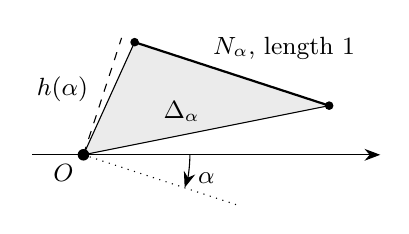
\begin{tikzpicture}[scale=2.6,>={Stealth[length=2mm]}]
  \coordinate (O) at (0,0);
  \coordinate (P) at (0.25,0.55);
  \coordinate (Q) at (1.20,0.24);
  % foot of perpendicular from O to the line through P and Q
  \coordinate (F) at (0.1863,0.5708);
  \fill[black!8] (O) -- (P) -- (Q) -- cycle;
  \draw[thick] (P) -- (Q);
  \draw (O) -- (P);
  \draw (O) -- (Q);
  \draw[dashed] (O) -- (F);
  \draw[->] (-0.25,0) -- (1.45,0);
  % direction of the needle, transported to O
  \draw[dotted] (O) -- (0.76,-0.248);
  \draw[->] (0.52,0) arc (0:-18:0.52);
  \node[font=\small] at (0.60,-0.115) {$\alpha$};
  \fill (O) circle (0.8pt) node[below left,font=\small]{$O$};
  \fill (P) circle (0.6pt);
  \fill (Q) circle (0.6pt);
  \node[above,font=\small] at (0.98,0.42) {$N_{\alpha}$, length $1$};
  \node[font=\small] at (0.48,0.21) {$\Delta_{\alpha}$};
  \node[left,font=\small] at (0.07,0.32) {$h(\alpha)$};
\end{tikzpicture}
\caption{The triangle reduction of Lemma~\ref{lem:triangle}. A needle
$N_{\alpha}\subset E$ in direction $\alpha\in\Tp$ forces the filled triangle
$\Delta_{\alpha}=\conv(\{O\}\cup N_{\alpha})\subset E$, of area $h(\alpha)/2$,
where $h(\alpha)$ is the distance from the star centre $O$ to the line of the
needle. The lower bound estimates the circular sections of an arbitrary such
family; the upper bound designs one such family and computes the radial envelope
of its union.}
\label{fig:triangle}
\end{figure}

\subsection{The two pipelines}\label{sec:pipelines}

Before any formula we describe what each half of the paper does with the
triangle family, in the order in which the quantities are produced.

\paragraph{Upper pipeline.}
\emph{Input:} two profiles $a,s$ on $[0,1]$ and an odd cell count $n$.
\emph{Goal:} one compact admissible set of area below the 1965 constant.
\emph{Mechanism:} the profiles determine one cell of a turning motion; joining
and reflection identities glue $n$ rotated copies into a half-turn, and odd
parity reverses the ordered endpoints. A package of sign conditions on $a$ and
$s$ forces the limiting radial envelope of the swept union to be the maximum of
a stationary branch and an endpoint branch. Exact elimination isolates the five
crossings of the two branches, polynomial antiderivatives evaluate the limiting
area, and a uniform $O(n^{-2})$ excess estimate transfers the bound to the
literal finite union. \emph{Output:} Theorem~\ref{thm:upper}.

\paragraph{Lower pipeline, baseline route.}
\emph{Input:} an arbitrary star-shaped Kakeya set with a pointwise chosen needle
family. \emph{Goal:} a strict area bound valid for every such set.
\emph{Mechanism:} a height threshold $h_{0}$ splits off the case of one large
triangle. Otherwise all heights are capped, and a radius $R_{1}$ splits the
direction circle into the confined and the escaping class; one of the two must
carry a prescribed share of direction mass. Confined directions are converted
into angular sections through first arcs, a same-centre dilation on $\Tp$ and
polar slicing; escaping directions are converted into disjoint exterior
triangles through a fixed-radius greedy deletion. \emph{Output:}
Theorem~\ref{thm:lower}.

\paragraph{Lower pipeline, additive refinement.}
\emph{Input:} the same arbitrary set and family, and the first-arc machinery of
the baseline route. \emph{Goal:} the same kind of bound with a larger constant.
\emph{Mechanism:} the height threshold $\hat h_{0}$ again splits off one large
triangle; otherwise a measurable closed ball of radius $\hat r_{0}$ splits the
plane. The confined class pays the raw radial integral inside that ball, with no
local-to-global conversion; the escaping class pays outside it, through the
exterior parts of greedily selected triangles, which are kept disjoint by
one-sided angular shadows, and through the annular fan of the directions that
survive every deletion. Carath\'eodory splitting adds the two payments, and
subadditivity of direction mass replaces the mass split. \emph{Output:}
Theorem~\ref{thm:annular}.

Table~\ref{tab:flow} records how a geometric hypothesis becomes area in each
half. The two pipelines share only Lemma~\ref{lem:triangle} and the final
infimum step of Section~\ref{sec:assembly}.

\begin{table}[t]
\centering
\small
\begin{tabular}{@{}lll@{}}
\toprule
Upper: quantity flow & Lower, baseline & Lower, refinement \\
\midrule
profiles $a,s$, cell count $n$
  & heights $h(\alpha)$
  & heights $h(\alpha)$\\
joining, reflection, odd parity
  & threshold $h_{0}$: high or cap
  & threshold $\hat h_{0}$: high or cap\\
sign package \eqref{eq:signs}--\eqref{eq:J}
  & radius $R_{1}$: mass split $p$
  & ball $\overline B(0,\hat r_{0})$: plane split\\
two branches $\Rsta,\Rend$
  & $g(r)$ / exterior ball $\rho$
  & $\hat g(r)$ / exterior ball $\hat\rho$\\
five switches, six intervals
  & $\pi p/g(r)$ / $c\kappa H(\delta)$
  & $L_{\mathrm{in}}/\hat g(r)$ /
    $\hat C_{\mathrm{ext}}\hat H(\delta)$\\
polynomial primitives, area
  & polar slicing / deletion budget
  & polar slicing / exterior ledger\\
finite-cell excess $\eta_{n}$
  & conversion $k$ / residual fan
  & Carath\'eodory split / annular fan\\
area of $E_{100001}$
  & $\Lout(E)>100\pi/5599$
  & $\Lout(E)>131\pi/6250$\\
\bottomrule
\end{tabular}
\caption{How each half converts its geometric hypothesis into planar area. The
left column is a design computation for one set; the other two are estimates
valid for every set, differing in how the confined and the escaping class are
combined.}
\label{tab:flow}
\end{table}

\subsection{Notation and its scope}

Table~\ref{tab:notation} lists the symbols together with the part of the paper
in which they are in force. Symbols that would otherwise carry two unrelated
meanings have been given distinct names:

\begin{itemize}
  \item $a(t)$ is the tangential profile of the construction in
    Part~\ref{part:upper}; the fixed rational height threshold of
    Part~\ref{part:lower} is written $h_{0}=1123/10000$;
  \item $\Hsup(t)=\tfrac12+a(t)$ is the support profile in
    Part~\ref{part:upper}; the triangle height function of
    Part~\ref{part:lower} keeps the name $h(\alpha)$;
  \item $s(t)$ is the normal profile in Part~\ref{part:upper}; the half-span of
    a first arc in Part~\ref{part:lower} is written $w_{\alpha}$;
  \item $\delta_{n}=\pi/n$ is the cell angle in Part~\ref{part:upper}, while
    $\delta$ in Part~\ref{part:lower} denotes a needle height;
  \item $\varepsilon=1/5$ is the profile perturbation amplitude in
    Part~\ref{part:upper}; the greedy deletion tolerance of
    Part~\ref{part:lower} is written $\epsdel=10^{-10}$;
  \item every constant of the additive refinement of
    Sections~\ref{sec:additive} and~\ref{sec:annbudget} carries a hat: the
    parameters $\hat h_{0}$, $\hat r_{\lambda}$, $\hat r_{0}$, the derived
    radii $\hat R_{1}$, $\hat\rho$, and the quantities $\hat g$, $\hat I$,
    $\hat T$ are never confused with the baseline $h_{0}$, $r_{\lambda}$,
    $r_{0}$, $R_{1}$, $\rho$, $g$, $I$, $T$ of \eqref{eq:params}, which they do
    not replace.
\end{itemize}
The stationary and endpoint branch parameters of the upper construction are
written $\tau$ and $\zeta$ (they are called \lean{p} and \lean{z} in the
formalisation) so as not to collide with the direction-mass proportion $p$ of
the lower proof, and the union of the chosen triangles of an arbitrary set $E$
is written $\Tri(E)$.

\begin{table}[t]
\centering
\small
\begin{tabular}{@{}lll@{}}
\toprule
Symbol & Meaning & Scope \\
\midrule
$\Tp$ & projective direction circle $\R/\pi\Z$, mass $\pi$ & throughout\\
$\Lout,\Lone$ & planar / directional outer measure & throughout\\
$\Delta_{\alpha},h(\alpha)$ & chosen triangle and its height
  & Part~\ref{part:lower}\\[2pt]
$n,\delta_{n},\sigma$ & cell count, $\pi/n$, $\pi-\delta_{n}$
  & Part~\ref{part:upper}\\
$a(t),s(t),\Hsup(t)$ & tangential, normal, support profiles
  & Part~\ref{part:upper}\\
$A,B,\varepsilon$ & odd/even perturbation polynomials, amplitude $1/5$
  & Part~\ref{part:upper}\\
$\tau,\zeta$ & stationary / endpoint branch parameters & Part~\ref{part:upper}\\
$\Rsta,\Rend,R$ & branch radii and their maximum & Part~\ref{part:upper}\\
$J$ & endpoint Jacobian $\Hsup^{2}-s'\Hsup+s\Hsup'$
  & Part~\ref{part:upper}\\
$\eta_{n}$ & finite-cell radial excess & Section~\ref{sec:finitelift}\\[2pt]
$\Tri(E)$ & union of the chosen triangles & Part~\ref{part:lower}\\
$h_{0},r_{\lambda},r_{0},p,\lambda$ & fixed rational lower-bound parameters
  & Part~\ref{part:lower}\\
$Q,d,R_{1},\rho$ & derived radii, $\rho=R_{1}-1$ & Part~\ref{part:lower}\\
$T$ & baseline lower target $100/5599$ & Part~\ref{part:lower}\\
$\Ain(R_{1}),\Aout(R_{1})$ & confined / escaping direction classes
  & Part~\ref{part:lower}\\
$g(r)$ & three-branch dilation factor at radius $r$ & Section~\ref{sec:caseI}\\
$I,\Istar$ & radial integral $\int_{h_{0}}^{r_{0}}r/g$ and its certified
  rational lower bound & Section~\ref{sec:caseI}\\
$f_{0},k,A_{0},X,X_{*},Y$ & conversion and branch coefficients
  & Part~\ref{part:lower}\\
$c,\kappa,H(\delta),\epsdel$ & exterior weight data, tolerance $10^{-10}$
  & Section~\ref{sec:caseII}\\[2pt]
$\hat h_{0},\hat r_{\lambda},\hat r_{0},\hat\lambda$ & refinement parameter
  tuple \eqref{eq:annparams} & Sections~\ref{sec:additive}--\ref{sec:annbudget}\\
$\hat Q,\hat d,\hat R_{1},\hat\rho$ & derived radii of the refinement,
  $\hat\rho=\hat R_{1}-1$ & Sections~\ref{sec:additive}--\ref{sec:annbudget}\\
$\hat g,\hat I,\hat T$ & refinement dilation loss, radial gain, target
  $131/6250$ & Sections~\ref{sec:additive}--\ref{sec:annbudget}\\
$\hat H(\delta),W_{\hat\rho}(\delta)$ & weighted half-width and sharp one-sided
  aperture & Section~\ref{sec:additive}\\
$\hat C_{\mathrm{ext}},\hat C_{\mathrm{fan}},\hat C_{\mathrm{out}}$ & exterior
  payment, fan and combined coefficients & Sections~\ref{sec:additive}--\ref{sec:annbudget}\\
$L_{\mathrm{in}},L_{\mathrm{out}}$ & direction masses of
  $\Ain(\hat R_{1})$, $\Aout(\hat R_{1})$
  & Sections~\ref{sec:additive}--\ref{sec:annbudget}\\
\bottomrule
\end{tabular}
\caption{Notation, with the scope in which each symbol is in force. Symbols
whose two readings could be confused have been given distinct names: $a(t)$
versus $h_{0}$, $\Hsup(t)$ versus $h(\alpha)$, $s(t)$ versus $w_{\alpha}$,
$\delta_{n}$ versus $\delta$, and $\varepsilon$ versus $\epsdel$. The hatted
block is the additive refinement; its constants are numerically different from
their unhatted baseline counterparts and never replace them.}
\label{tab:notation}
\end{table}

% =====================================================================
\part{The explicit upper construction}\label{part:upper}

% ---------------------------------------------------------------------
\section{Designing the profiles and the odd-cycle assembly}
\label{sec:construction}

\emph{Input:} the classical one-cell mechanism of \cite{CunninghamSchoenberg1965}.
\emph{Goal:} a symmetry-restricted polynomial design space of turning
constructions inside which a single member can be certified exactly. \emph{Mechanism:} write the motion in
line-space coordinates, impose the cell-joining and reflection identities,
restrict to polynomial perturbations of the classical baseline, and record the
sign conditions that the later envelope analysis needs. \emph{Output:} an
explicit profile pair, and, for every odd $n$, an admissible compact set $E_{n}$.

\subsection{Cell kinematics and the classical baseline}

The construction is most naturally described in line-space coordinates. Let
$n$ be an odd positive integer and put
\[
  \delta_{n}=\frac{\pi}{n},\qquad \sigma=\pi-\delta_{n},
  \qquad
  u(t)=e(\delta_{n} t),\qquad \nu(t)=e\bigl(\delta_{n} t-\tfrac{\pi}{2}\bigr),
\]
so that $\nu(t)$ is the clockwise normal of $u(t)$. During one angular cell the
unit segment has direction $u(t)$ and centre
\begin{equation}\label{eq:c0}
  c_{0}(t)=a(t)\,u(t)+\frac{\pi\,s(t)}{n}\,\nu(t),
  \qquad 0\le t\le 1 .
\end{equation}
The first term records how far the segment slides along its own direction, the
second how far it is displaced sideways. The scaling $\pi/n$ of the normal term
keeps the sideways displacement at cell scale; it is what makes the ratio
$s/D$ appear in the limit $n\to\infty$ and makes the finite correction of
Section~\ref{sec:finitelift} quadratic in $1/n$. Finally
\begin{equation}\label{eq:hprofile}
  \Hsup(t)=\tfrac12+a(t)
\end{equation}
is the \emph{support profile}: it is the distance from the origin to the leading
endpoint measured along $u(t)$, and it is the quantity the endpoint contacts of
Section~\ref{sec:envelope} see.

The linear tangential and parabolic normal pair
\begin{equation}\label{eq:baseline}
  a_{0}(t)=\frac{1-2t}{2\sqrt2},
  \qquad
  s_{0}(t)=\frac{t(1-t)}{4-2\sqrt2}
\end{equation}
is the cell underlying the Cunningham--Schoenberg mechanism, whose limiting
areas approach $(5-2\sqrt2)\pi/24$. We perturb this pair, keeping the cell
structure intact.

\subsection{Joining and reflection constraints}

Consecutive cells are glued by a rotation combined with a reflection of the cell
parameter, so continuity of the assembled motion is a constraint on the profiles
before any coefficient is chosen. Reflecting a cell sends $t$ to $1-t$; the
terminal data of one cell must be the initial data of the next, for the centre
and for the \emph{ordered} segment. This asks exactly for
\begin{equation}\label{eq:reflect}
  a(1-t)=-a(t),\qquad s(1-t)=s(t),\qquad s(0)=s(1)=0 .
\end{equation}
Put $v=2t-1$, so that $t\mapsto1-t$ becomes $v\mapsto-v$. Then \eqref{eq:reflect}
says that $a$ is odd and $s$ is even in $v$, and that the normal displacement
vanishes at both cell interfaces. Both requirements are met by the baseline
\eqref{eq:baseline}, and they are preserved by the perturbation ansatz
\begin{equation}\label{eq:ansatz}
  a=a_{0}+\varepsilon\, t(1-t)\,A(v),
  \qquad
  s=s_{0}\bigl(1+\varepsilon B(v)\bigr),
  \qquad A\text{ odd},\ B\text{ even},
\end{equation}
because the factor $t(1-t)$ vanishes at $t=0,1$ and therefore leaves the
interface values of $a$ unchanged, while multiplying $s_{0}$ by an even factor
preserves both the parity and the vanishing at the interfaces. Thus the parity
of $A$ and $B$ and the endpoint factor $t(1-t)$ in \eqref{eq:ansatz} are imposed
by the geometry of the assembly; only the polynomials $A,B$ and the amplitude
$\varepsilon$ remain free.

Restricting $A$ and $B$ to polynomials cuts the admissible perturbations down
to a symmetry-restricted polynomial design space, and has a further consequence
used throughout: the contact equations of Section~\ref{sec:envelope} then stay
algebraic over $\Q(\sqrt2)$, so branch crossings can be isolated by exact
elimination and each branch area is a polynomial antiderivative.

\subsection{Shape conditions demanded by the contact geometry}
\label{sec:signrole}

The envelope analysis of Section~\ref{sec:envelope} needs the profiles to have a
definite shape. We state the required inequalities here, before choosing
coefficients, together with the role each of them plays. On the closed cell
parameter interval $0\le t\le1$ we ask for
\begin{equation}\label{eq:signs}
  s''<0,\qquad \Hsup>0,\qquad \Hsup'<0,\qquad \Hsup-s'>0,
  \qquad\text{and}\qquad s(t)>0\ \ (0<t<1),
\end{equation}
the last only on the open interval because $s$ vanishes at both cell
interfaces by \eqref{eq:reflect}, together with the positivity of the endpoint
Jacobian on all of $[0,1]$,
\begin{equation}\label{eq:J}
  J(t):=\Hsup(t)^{2}-s'(t)\Hsup(t)+s(t)\Hsup'(t)>0 .
\end{equation}
Their roles are:
\begin{itemize}
  \item $s>0$: the normal displacement is a genuine arch, so the swept cell has
    a nondegenerate outer boundary;
  \item $s''<0$: strict concavity makes the stationary contact map
    $\tau\mapsto s(\tau)/s'(\tau)-\tau$ strictly monotone and eliminates all
    shifted stationary competitors, leaving one stationary branch;
  \item $\Hsup>0$ and $\Hsup'<0$: the endpoint cap seen by a radial contact is positive
    and decreasing, which is what disposes of the unshifted endpoint candidate
    of the wrong sign;
  \item $\Hsup-s'>0$: feasibility of the endpoint branch, i.e.\ the endpoint contact
    actually occurs in the parameter range where it is claimed;
  \item $J>0$: the endpoint coordinate map $\zeta\mapsto\zeta-s(\zeta)/\Hsup(\zeta)$
    is strictly increasing, so the endpoint change of variables in
    Section~\ref{sec:envelope} is legitimate and its area density is positive.
\end{itemize}
Together, \eqref{eq:signs}--\eqref{eq:J} supply the principal monotonicity and
feasibility inputs of the contact classification. They do not by themselves
close it: the reduction of an a priori infinite lattice of candidate contacts to
two branches (Proposition~\ref{prop:branches}) also uses the reflection
identities \eqref{eq:reflect}, the endpoint values $s(0)=s(1)=0$, the parameter
ranges recorded there, and explicit comparisons between the shifted and
unshifted candidates.

\subsection{An explicit profile pair}

Within the constrained family \eqref{eq:ansatz} we now fix one member. It was
located by computational exploration of that family; no optimality, minimality
of degree, or uniqueness is claimed for it, and no derivation identifying it as
the solution of an optimisation problem is offered. Everything after this
subsection is exact certification of the displayed data.

We take the amplitude $\varepsilon=1/5$ and the two rational polynomials
\begin{align}
  A(v)&=-\frac{7}{80}v+\frac{1}{9}v^{3}-\frac{1}{160}v^{5},
  \label{eq:Apoly}\\[2pt]
  B(v)&=\frac{1}{68}-\frac{41}{120}v^{2}+v^{4}-\frac{20}{27}v^{6},
  \label{eq:Bpoly}
\end{align}
so that \eqref{eq:ansatz} becomes
\begin{align}
  a(t)&=\frac{1-2t}{2\sqrt2}+\frac15\,t(1-t)\,A(2t-1),
  \label{eq:aprofile}\\[2pt]
  s(t)&=\frac{t(1-t)}{4-2\sqrt2}\Bigl(1+\frac15B(2t-1)\Bigr),
  \qquad 0\le t\le1 ,
  \label{eq:sprofile}
\end{align}
with $\Hsup=\tfrac12+a$ as in \eqref{eq:hprofile}. The coefficients lie in $\Q$ and
the profiles in $\Q(\sqrt2)[t]$.

\begin{proposition}[profile shape inequalities]\label{prop:signs}
The profiles \eqref{eq:aprofile}--\eqref{eq:sprofile} satisfy
\eqref{eq:reflect}. Moreover $s''<0$, $\Hsup>0$, $\Hsup'<0$, $\Hsup-s'>0$ and
$J>0$ hold at every $t\in[0,1]$, and $s(t)>0$ for every $t\in(0,1)$.
\end{proposition}

\begin{proof}
The identities \eqref{eq:reflect} hold because $A$ is odd and $B$ is even in
$v=2t-1$. Each remaining assertion is a strict sign for an explicit polynomial
in $\Q(\sqrt2)[t]$ on a closed rational interval; these signs are established by
exact Sturm certificates over $\Q(\sqrt2)$ together with Bernstein/Horner
enclosures with rational endpoints, described in Appendix~\ref{app:constants}
and checked formally as recorded in Appendix~\ref{app:formalization}. For $s$
itself the certificate is applied to $s(t)/(t(1-t))$, which is strictly positive
on all of $[0,1]$.
\end{proof}

Figure~\ref{fig:profiles} plots the three profiles.

\begin{figure}[t]
\centering
\begin{tikzpicture}[x=9.2cm,y=4.6cm]
  \draw[->] (0,0) -- (1.06,0) node[below]{$t$};
  \draw[->] (0,-0.42) -- (0,0.95);
  \foreach \x in {0,0.25,0.5,0.75,1}
    \draw (\x,0) -- (\x,-0.018) node[below,font=\scriptsize]{$\x$};
  \foreach \y in {-0.4,-0.2,0.2,0.4,0.6,0.8}
    \draw (0,\y) -- (-0.008,\y) node[left,font=\scriptsize]{$\y$};
  % Hsup(t)
  \draw[very thick]
    (0.000,0.8536) -- (0.050,0.8182) -- (0.100,0.7831) --
    (0.150,0.7481) -- (0.200,0.7131) -- (0.250,0.6779) -- (0.300,0.6426) --
    (0.350,0.6071) -- (0.400,0.5715) -- (0.450,0.5358) -- (0.500,0.5000) --
    (0.550,0.4642) -- (0.600,0.4285) -- (0.650,0.3929) -- (0.700,0.3574) --
    (0.750,0.3221) -- (0.800,0.2869) -- (0.850,0.2519) -- (0.900,0.2169) --
    (0.950,0.1818) -- (1.000,0.1464);
  \node[right,font=\small] at (1.005,0.15) {$\Hsup$};
  % a(t)
  \draw[thick,dashed]
    (0.000,0.3536) -- (0.050,0.3182) -- (0.100,0.2831) -- (0.150,0.2481) --
    (0.200,0.2131) -- (0.250,0.1779) -- (0.300,0.1426) -- (0.350,0.1071) --
    (0.400,0.0715) -- (0.450,0.0358) -- (0.500,0.0000) -- (0.550,-0.0358) --
    (0.600,-0.0715) -- (0.650,-0.1071) -- (0.700,-0.1426) -- (0.750,-0.1779) --
    (0.800,-0.2131) -- (0.850,-0.2481) -- (0.900,-0.2831) -- (0.950,-0.3182) --
    (1.000,-0.3536);
  \node[right,font=\small] at (1.005,-0.355) {$a$};
  % s(t)
  \draw[thick,dotted]
    (0.000,0.0000) -- (0.050,0.0405) -- (0.100,0.0770) -- (0.150,0.1088) --
    (0.200,0.1362) -- (0.250,0.1594) -- (0.300,0.1786) -- (0.350,0.1939) --
    (0.400,0.2050) -- (0.450,0.2117) -- (0.500,0.2140) -- (0.550,0.2117) --
    (0.600,0.2050) -- (0.650,0.1939) -- (0.700,0.1786) -- (0.750,0.1594) --
    (0.800,0.1362) -- (0.850,0.1088) -- (0.900,0.0770) -- (0.950,0.0405) --
    (1.000,0.0000);
  \node[font=\small] at (0.5,0.245) {$s$};
\end{tikzpicture}
\caption{The three profiles \eqref{eq:aprofile}, \eqref{eq:sprofile} and
\eqref{eq:hprofile} on
$[0,1]$, sampled at steps of $0.05$ from their exact formulas: the tangential
profile $a$ (dashed, odd about $t=\tfrac12$, with $a(0)=1/(2\sqrt2)$), the
normal profile $s$ (dotted, even, vanishing at both endpoints) and the support
profile $\Hsup=\tfrac12+a$ (solid, positive and strictly decreasing). The signs
\eqref{eq:signs} are proved by exact certificates
(Proposition~\ref{prop:signs}), not read off this plot.}
\label{fig:profiles}
\end{figure}

\subsection{The odd cycle}

Let $R_{\phi}$ denote clockwise rotation of $\R^{2}$ by the angle $\phi$ about
the origin. For $j=0,1,\dots,n-1$ put
\begin{equation}\label{eq:cells}
  c_{j}(t)=R_{j\sigma}c_{0}(t),\qquad
  d_{j}(t)=(-1)^{j}R_{j\sigma}u(t),
\end{equation}
\[
  p_{j}(t)=c_{j}(t)-\tfrac12 d_{j}(t),\qquad
  q_{j}(t)=c_{j}(t)+\tfrac12 d_{j}(t),
\]
and define the literal set
\begin{equation}\label{eq:Edef}
  E_{n}
  :=\bigcup_{j=0}^{n-1}\ \bigcup_{0\le t\le 1}
    \conv\bigl\{0,\;p_{j}(t),\;q_{j}(t)\bigr\}.
\end{equation}
Equivalently, $E_{n}$ is the set of points
$\lambda\bigl((1-r)p_{j}(t)+rq_{j}(t)\bigr)$ with
$\lambda,r,t\in[0,1]$ and $0\le j\le n-1$: a finite union of swept filled
triangles, not a limiting envelope and not a sampled approximation.

The projective direction of $d_{j}(t)$ is
\[
  \delta_{n} t-j\sigma\equiv \delta_{n}(t+j)\pmod{\pi},
\]
so that, as $j$ runs through $0,\dots,n-1$ and $t$ through $[0,1]$, the
direction sweeps the full projective circle exactly once, monotonically, in
steps of $\delta_{n}=\pi/n$ per cell. This is the sense in which the construction is
a genuine half-turn, and it is what the global angular parameter
$\theta=\delta_{n}(j+t)\in[0,\pi]$ records. See Figure~\ref{fig:oddcycle}.

\begin{figure}[t]
\centering
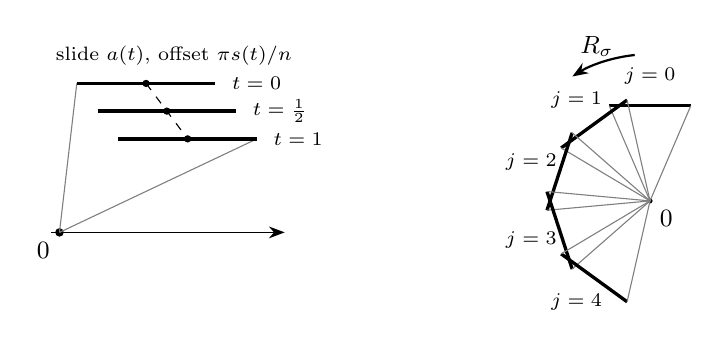
\begin{tikzpicture}[scale=1.0,>={Stealth[length=2mm]}]
  % ---------- left panel: one cell
  \begin{scope}[shift={(-4.6,-0.1)},scale=2.2]
    \draw[->] (-0.05,0) -- (1.30,0);
    \fill (0,0) circle (0.7pt) node[below left,font=\small]{$0$};
    \draw[gray] (0,0) -- (0.10,0.86);
    \draw[gray] (0,0) -- (1.14,0.54);
    \draw[very thick] (0.10,0.86) -- (0.90,0.86);
    \draw[very thick] (0.22,0.70) -- (1.02,0.70);
    \draw[very thick] (0.34,0.54) -- (1.14,0.54);
    \fill (0.50,0.86) circle (0.6pt);
    \fill (0.62,0.70) circle (0.6pt);
    \fill (0.74,0.54) circle (0.6pt);
    \draw[dashed] (0.50,0.86) -- (0.74,0.54);
    \node[font=\scriptsize,right] at (0.94,0.86) {$t=0$};
    \node[font=\scriptsize,right] at (1.06,0.70) {$t=\tfrac12$};
    \node[font=\scriptsize,right] at (1.18,0.54) {$t=1$};
    \node[font=\scriptsize] at (0.66,1.02) {slide $a(t)$, offset $\pi s(t)/n$};
  \end{scope}
  % ---------- right panel: odd cycle, schematic with a small odd n
  \begin{scope}[shift={(2.9,0.30)},scale=1.15]
    \fill (0,0) circle (0.8pt) node[below right,font=\small]{$0$};
    \foreach \k in {0,1,2,3,4}{
      \begin{scope}[rotate=\k*36]
        \draw[very thick] (-0.45,1.05) -- (0.45,1.05);
        \draw[gray] (0,0) -- (-0.45,1.05);
        \draw[gray] (0,0) -- (0.45,1.05);
      \end{scope}
      \node[font=\scriptsize] at ({90+\k*36}:1.38) {$j=\k$};}
    \draw[->,thick] (96:1.62) arc (96:122:1.62);
    \node[font=\small] at (109:1.80) {$R_{\sigma}$};
  \end{scope}
\end{tikzpicture}
\caption{Schematic of the construction. Left: one cell. The unit segment slides
tangentially by $a(t)$ and is displaced normally by $\pi s(t)/n$ (the normal
displacement is exaggerated); the swept triangles with apex at the origin are
indicated by the two grey rays. Right: the odd cycle. Cell $j$ is the clockwise
rotation by $j\sigma$ of cell $0$, with the direction sign flipped when $j$ is
odd, so the projective direction advances by $\delta_{n}=\pi/n$ per cell. The
right-hand panel is drawn with a small odd cell count for legibility; the cell
count is fixed only in Section~\ref{sec:finitelift}.}
\label{fig:oddcycle}
\end{figure}

\subsection{Admissibility}

\begin{proposition}[admissibility]\label{prop:admissible}
For every odd $n\ge1$ the set $E_{n}$ of \eqref{eq:Edef} is compact,
star-shaped about the origin, and carries a continuous turning needle in the
sense of Definition~\ref{def:turning}. In particular $E_{n}$ is admissible and
is a star-shaped Kakeya set.
\end{proposition}

\begin{proof}
The reflection identities \eqref{eq:reflect} give the \emph{joining identities}
at the cell interface: the terminal data of cell $j$ at $t=1$ coincide with the
initial data of cell $j+1$ at $t=0$, both for the centre and, thanks to the
parity factor $(-1)^{j}$ in \eqref{eq:cells}, for the ordered unit segment.
Hence the two endpoint maps
\[
  p(\theta)=p_{j}(t),\qquad q(\theta)=q_{j}(t),
  \qquad \theta=\delta_{n}(j+t),
\]
are well defined and continuous on $[0,\pi]$, and satisfy
$q(\theta)-p(\theta)=e(\theta)$ identically. Because $n$ is odd, after all $n$
cells the centre returns to its initial position while the oriented direction has
changed sign; this is exactly the reversal $p(\pi)=q(0)$, $q(\pi)=p(0)$. Each
moving segment lies in its own origin-based triangle, hence in $E_{n}$, so the
containment requirement holds. Star-shapedness about $0$ is immediate from
\eqref{eq:Edef}: each triangle contains $0$ and is closed under radial
contraction towards $0$. Finally, each cell is the image of the compact cube
$[0,1]^{3}$ under a continuous map, and there are finitely many cells, so
$E_{n}$ is compact, hence bounded and measurable. Routine continuity
verifications at the cell interfaces are carried out in the formalisation for
the literal set \eqref{eq:Edef}.
\end{proof}

\begin{remark}\label{rem:parity}
The parity of $n$ is used only in the reversal step, but it is used essentially:
for even $n$ the same cell data close up into a full turn without exchanging the
ordered endpoints, so Definition~\ref{def:turning} would fail. Oddness is thus
an admissibility requirement, whereas the size of $n$ is a purely quantitative
matter, settled in Section~\ref{sec:finitelift}. Proposition~\ref{prop:admissible}
is stated here for every odd $n$; the formal development instantiates it at the
single value $n=100001$ used by Theorem~\ref{thm:upper}, and proves no statement
quantified over $n$.
\end{remark}

The construction is now admissible for every odd $n$; it remains to estimate its
area, which we do first in the limit $n\to\infty$.

% ---------------------------------------------------------------------
\section{The continuum radial envelope and its exact area decomposition}
\label{sec:envelope}

\emph{Input:} the profile pair of Section~\ref{sec:construction} and its shape
inequalities. \emph{Goal:} an exact rational upper bound for the area swept in
the limit $n\to\infty$. \emph{Mechanism:} classify all limiting contacts of a
ray with the swept family, reduce them to two branches, locate every crossing of
the two branches, and integrate each active branch by a polynomial
antiderivative. \emph{Output:} the strict bound \eqref{eq:contbound}.

\subsection{Two branches and their completeness}

Let $y=x/\pi\in[0,1]$ be the normalised coordinate on a fundamental angular
sector of the construction, obtained after the reflection and cyclic folds
described in Section~\ref{sec:finitelift}. As $n\to\infty$ the radial extent of
the star hull in the direction $y$ is governed by two families of contacts:
\begin{itemize}
  \item a \emph{stationary} branch, where the ray is tangent to the family of
    supporting lines of the moving segment; and
  \item an \emph{endpoint} branch, where the ray meets a moving endpoint.
\end{itemize}
Concretely, the stationary branch is parametrised by $\tau$ through
\begin{equation}\label{eq:stationary}
  y=\frac{s(\tau)}{s'(\tau)}-\tau,\qquad \Rsta(y)=s'(\tau),
\end{equation}
and the endpoint branch by $\zeta$ through
\begin{equation}\label{eq:endpoint}
  y=\zeta-\frac{s(\zeta)}{\Hsup(\zeta)},\qquad \Rend(y)=\Hsup(\zeta).
\end{equation}
The endpoint map $\zeta\mapsto\zeta-s(\zeta)/\Hsup(\zeta)$ has derivative
$J(\zeta)/\Hsup(\zeta)^{2}>0$, so by Proposition~\ref{prop:signs} it is an
increasing bijection of $[0,1]$ onto $[0,1]$ and $\zeta=\zeta(y)$ is uniquely
determined for every $y\in[0,1]$. On the stationary side the parameter runs over
$[0,\tau_{*}]$, where $\tau_{*}$ is the unique solution of
\begin{equation}\label{eq:taustar}
  s(\tau_{*})=(1+\tau_{*})\,s'(\tau_{*}),
  \qquad \tau_{*}=0.4188076\ldots<\tfrac12,
\end{equation}
that is, the stationary parameter carrying $y=1$; $\tau=\tau(y)$ is again unique
because $s''<0$.

A priori a fixed ray has many more candidate contacts than these two: the swept
family is invariant under the cell lattice, so each contact type reappears with
every cell shift $\ell$ and with either sign. The following proposition says
that all of them are dominated by
\eqref{eq:stationary}--\eqref{eq:endpoint}.

\begin{proposition}[branch completeness]\label{prop:branches}
The limiting radial majorant on the fundamental sector is
\begin{equation}\label{eq:Rmax}
  R(y)=\max\{\Rsta(y),\Rend(y)\},\qquad 0\le y\le1 .
\end{equation}
\end{proposition}

\begin{proof}
Fix $y\in(0,1)$. For the \emph{plus} branch with shift $\ell=0$, the radial
ratio is $f_{y}(t)=s(t)/(y+t)$, whose derivative has numerator
$s'(t)(y+t)-s(t)$; this numerator has derivative $s''(t)(y+t)<0$ and is positive
at $t=0$, so it has a unique zero $\tau=\tau(y)$, which is therefore the unique
unconstrained maximiser, and there \eqref{eq:stationary} holds. That this
maximiser is strictly feasible is exactly $\Hsup(\tau)-s'(\tau)>0$. Every plus
shift $\ell\le-1$ has a strictly larger positive denominator and is therefore
dominated, and plus shifts $\ell\ge1$ are invalid in the open half-sector.
Hence $\Rsta$ is the complete plus-branch maximum.

For the \emph{minus} branch with shift $\ell=0$ put $z=1-t$. The reflection
identities \eqref{eq:reflect} turn its ratio and half-length constraint into
$s(z)/(z-y)\le\Hsup(z)$, so feasibility is exactly $z\ge\zeta(y)$. On the
feasible interval, the derivative of $s(z)/(z-y)$ has numerator
$s'(z)(z-y)-s(z)$, which is nonpositive for $z\le\tfrac12$ by concavity and
$s(0)=0$, and negative for $z\ge\tfrac12$ because there $s'(z)\le0$. Hence the
shift-$0$ minus branch is maximised at the boundary of its feasible interval,
and this \emph{retained} boundary contact is precisely the endpoint branch
$\Rend(y)=\Hsup(\zeta(y))$ of \eqref{eq:endpoint}.

For a minus shift $\ell\ge1$ the denominator is $z-y+2\ell\ge1+z$, so the ratio
is at most $s(z)/(1+z)$, which is maximised by the stationary branch at $y=1$;
since $\Rsta$ is decreasing in $y$, every such branch is bounded by
$\Rsta(1)\le\Rsta(y)$. Negative minus shifts are invalid. No lattice shift can
therefore enlarge the envelope, and \eqref{eq:Rmax} follows. The classification
is carried out for the explicit profiles and is checked formally; see
Appendix~\ref{app:formalization}.
\end{proof}

\subsection{The switch system}

To integrate $\max\{\Rsta,\Rend\}$ we must know every point at which the two
branches exchange dominance and which branch is active in between. The two
branches meet where $\Rsta=\Rend$ and the corresponding $y$-values agree, that
is, at solutions of the system
\begin{equation}\label{eq:switch}
  s'(\tau)=\Hsup(\zeta),
  \qquad
  s(\tau)+s(\zeta)=(\tau+\zeta)\,s'(\tau).
\end{equation}

\begin{lemma}[switch isolation]\label{lem:switch}
The system \eqref{eq:switch} has exactly five solutions
$(\tau_{i},\zeta_{i})$, $i=0,\dots,4$, in the interior of the switch rectangle
$[0,\tau_{*}]\times[0,1]$, with $\tau_{*}$ as in \eqref{eq:taustar}. Writing
$y_{0}<y_{1}<\dots<y_{4}$ for the corresponding switch abscissae, the active
branch on the six intervals
\[
  [0,y_{0}],\;[y_{0},y_{1}],\;[y_{1},y_{2}],\;
  [y_{2},y_{3}],\;[y_{3},y_{4}],\;[y_{4},1]
\]
is, in order,
\[
  \mathrm{e},\ \mathrm{s},\ \mathrm{e},\ \mathrm{s},\ \mathrm{e},\ \mathrm{s}.
\]
\end{lemma}

\begin{proof}
Exact elimination of \eqref{eq:switch} to a univariate resultant, rational root
isolation, and a subresultant/B\'ezout recovery of the second coordinate produce
five isolating boxes inside $[0,\tau_{*}]\times[0,1]$, of width below
$10^{-20}$, and prove that the system has no further solution there; the slope
differences are nonzero on all five boxes, so the crossings are simple; dominance of the
asserted branch on each of the six intervals is then a sign check on the
isolating boxes. All steps use exact rational isolating boxes and polynomial
identities; the certificate data are described in Appendix~\ref{app:constants}
and the formal statements in Appendix~\ref{app:formalization}. Decimal values of
the switches appear nowhere in the argument; any decimals printed by the
verification scripts are displays of certified rational enclosures.
\end{proof}

\subsection{Change of variables and the six-piece identity}

By reflection symmetry the limiting area is
\begin{equation}\label{eq:polar}
  \mathcal A_{\infty}=\pi\int_{0}^{1}R(y)^{2}\,dy .
\end{equation}
Differentiating \eqref{eq:stationary} and \eqref{eq:endpoint} and using
\eqref{eq:J} gives the exact densities
\begin{equation}\label{eq:densities}
  \Rsta(y)^{2}\,dy=-s(\tau)s''(\tau)\,d\tau,
  \qquad
  \Rend(y)^{2}\,dy=J(\zeta)\,d\zeta .
\end{equation}
Both densities lie in $\Q(\sqrt2)[t]$, and both are positive by
Proposition~\ref{prop:signs}; this is where $s''<0$ and $J>0$ are used
quantitatively rather than qualitatively. Let $\Ps$ and $\Pe$ be their
antiderivatives with zero constant term,
\[
  \Ps'=-s\,s'',\qquad \Pe'=J .
\]
Combining \eqref{eq:polar}, Lemma~\ref{lem:switch} and \eqref{eq:densities} on
the six intervals yields the exact identity
\begin{equation}\label{eq:sixpiece}
\begin{aligned}
  \frac{\mathcal A_{\infty}}{\pi}
  ={}&\Pe(\zeta_{0})-\Pe(0)
     +\Ps(\tau_{1})-\Ps(\tau_{0})\\
    &+\Pe(\zeta_{2})-\Pe(\zeta_{1})
     +\Ps(\tau_{3})-\Ps(\tau_{2})\\
    &+\Pe(\zeta_{4})-\Pe(\zeta_{3})
     +\Ps(\tau_{*})-\Ps(\tau_{4}).
\end{aligned}
\end{equation}

\begin{proposition}[continuum area bound]\label{prop:area}
Evaluating \eqref{eq:sixpiece} on the certified isolating boxes with outward
rounding gives the strict rational bound
\begin{equation}\label{eq:contbound}
  \int_{0}^{1}R(y)^{2}\,dy\ <\ \frac{90477812}{10^{9}} .
\end{equation}
\end{proposition}

\begin{proof}
Each of the twelve endpoint values in \eqref{eq:sixpiece} is the value of a
polynomial in $\Q(\sqrt2)[t]$ at a parameter confined to a certified rational
isolating box from Lemma~\ref{lem:switch}. Evaluating each polynomial on its box
with outward-rounded rational interval arithmetic and summing gives a rational
upper bound for the right-hand side of \eqref{eq:sixpiece}, which is then
compared with $90477812/10^{9}$ by exact rational arithmetic. The endpoint data
are listed in Appendix~\ref{app:constants}.
\end{proof}

The bound \eqref{eq:contbound} is deliberately rounded: an independent outward
interval computation gives
\[
  \frac{\mathcal A_{\infty}}{\pi}=0.0904778111246769545\ldots
\]
at the displayed precision. That decimal is a numerical report, not a theorem,
and is never used as an exact identity.

The limiting area is now certified; Section~\ref{sec:finitelift} transfers this
estimate to a literal finite union.

% ---------------------------------------------------------------------
\section{The finite-cell lift and the explicit upper bound}
\label{sec:finitelift}

\emph{Input:} the continuum envelope $R$ and its certified area bound.
\emph{Goal:} an area bound for a literal finite union \eqref{eq:Edef}.
\emph{Mechanism:} fold every ray into the fundamental sector, compare each
retained finite branch with its continuum limit, control the one branch that
exists only at finite cell count, fix one explicit odd cell count, and integrate
the resulting radial excess. \emph{Output:} Theorem~\ref{thm:upper}.

\subsection{Folding and the finite branch formulas}

The continuum envelope $R$ is only an intermediate majorant: the set $E_{n}$ is
a finite union, and its radial function may exceed $R$. Three structural
features govern the difference, and each contributes an error of order $n^{-2}$.

\emph{(a) Folding.} An explicit cyclic-and-reflection fold maps every ray of the
plane into the fundamental sector. The fold must be applied before any
small-angle estimate, because the raw positive denominator of an actual cell
contact may lie in $(n/2,n)$, so its angle is close to $\pi$ rather than acute;
every positive nonparallel contact folds to
$\widehat D=\min\{D,n-D\}\in(0,n/2]$, and the identities \eqref{eq:reflect}
together with $\sin(\pi-\cdot)=\sin(\cdot)$ show that this preserves the finite
radius and reflects the feasibility interval.

\emph{(b) Finite branch formulas and a tail cutoff.} On a retained finite branch
with positive folded denominator $D$ one sets $w=\pi D/n$ and has the exact
formulas
\begin{equation}\label{eq:finitebranch}
  R^{\mathrm{br}}_{\infty}=\frac{s(t)}{D},
  \qquad
  R^{\mathrm{br}}_{n}=R^{\mathrm{br}}_{\infty}\,\frac{w}{\sin w},
  \qquad
  T^{\mathrm{br}}_{n}=R^{\mathrm{br}}_{\infty}\,w\cot w .
\end{equation}
Since $\sin w\ge 2w/\pi$ on $(0,\pi/2]$, every folded branch with
$\widehat D\ge3$ has $R^{\mathrm{br}}_{n}\le\pi s_{\max}/6$ with
$s_{\max}=s(1/2)$, while the finite copy of a continuum active branch already
has radius at least $h_{\min}=\Hsup(1)$; the exact profile certificate gives
$\tfrac{11}{21}s_{\max}<h_{\min}$, so such branches cannot maximise. Hence every
maximising branch may be taken with $0<\widehat D<3$, and then
$w<q_{n}:=66/(7n)$ using $\pi<22/7$. On that range $w/\sin w\le(1-q_{n}^{2}/6)^{-1}$.

\emph{(c) Newly feasible branches.} At finite $n$ one branch that is infeasible
in the limit --- the shift-$0$ minus endpoint branch --- can become feasible. Its
angular displacement past the limiting feasibility threshold is bounded by
$\tfrac34q_{n}^{2}$, and a certified global Lipschitz bound $256$ for the
envelope $R$ converts this displacement into a radial excess of the same order.
All other branches are controlled by (b) or are strictly dominated below the
envelope.

Each of (a)--(c) is quadratic in $1/n$, which is the structural reason a finite
cell count suffices at all. We do not develop this into a bound valid for every
odd $n$; instead we fix one explicit cell count and certify the resulting
constants exactly.

\subsection{Choosing one explicit odd cell count}

Proposition~\ref{prop:area} bounds the continuum area independently of $n$, so
it suffices to choose an odd $n$ whose $O(n^{-2})$ allowance fits inside the
margin that bound leaves below the classical constant. We fix
\[
  n=100001 ,
\]
and write $E_{100001}$ for the corresponding literal set \eqref{eq:Edef}. Put
\begin{equation}\label{eq:qeta}
  q:=q_{100001}=\frac{66}{7\cdot100001},
  \qquad
  \eta:=\frac{(385/2)\,q^{2}}{1-q^{2}/2},
\end{equation}
so that $\eta$ is the exact rational number
\begin{equation}\label{eq:etaval}
  \eta=\frac{6930}{4049667751}=1.7113\ldots\times10^{-6}.
\end{equation}
The two roles of $n$ are distinct: \emph{oddness} is required for endpoint
reversal (Remark~\ref{rem:parity}), while the \emph{size} of $n$ is required
only for the error closure below. We do not assert that $100001$ is the smallest
odd cell count for which the estimate closes; it is one explicit value with a
comfortable margin, and it is the value carried by the formal development.

\subsection{The certified lift at the chosen cell count}

\begin{proposition}[finite-cell lift at $n=100001$]\label{prop:lift}
With $q$ and $\eta$ as in \eqref{eq:qeta}--\eqref{eq:etaval}, every ray of
$E_{100001}$ has radius at most $R+\eta$, where $R$ is the continuum envelope
\eqref{eq:Rmax} evaluated at the folded angular coordinate of the ray.
Consequently
\begin{equation}\label{eq:liftarea}
  \frac{|E_{100001}|}{\pi}
  \ \le\ \int_{0}^{1}R(y)^{2}\,dy+\bigl(2\eta+\eta^{2}\bigr).
\end{equation}
\end{proposition}

\begin{proof}
Fix a ray and fold it into the fundamental sector as in (a). By the tail cutoff
of (b), the ray may be assumed to realise its maximum on a branch with folded
denominator $\widehat D<3$, so $w<q$ and
\[
  R^{\mathrm{br}}_{n}-R^{\mathrm{br}}_{\infty}
  =R^{\mathrm{br}}_{\infty}\Bigl(\frac{w}{\sin w}-1\Bigr)
  \le R^{\mathrm{br}}_{\infty}\,\frac{q^{2}/6}{1-q^{2}/6},
\]
and $R^{\mathrm{br}}_{\infty}\le R$ for every branch that is feasible in the
limit, by Proposition~\ref{prop:branches}. For the branch of (c), finite
feasibility and $\cos w\ge1-w^{2}/2$ give
$R^{\mathrm{br}}_{n}=T^{\mathrm{br}}_{n}/\cos w$ and an angular displacement at
most $\tfrac34q^{2}$, which the Lipschitz bound $256$ converts into
$R^{\mathrm{br}}_{n}-R\le\eta$. This last estimate dominates the previous one,
which gives the pointwise bound $R+\eta$; the terminal rational arithmetic at
$n=100001$ is recorded in Appendix~\ref{app:constants}. Only the branch data,
ranges and constants of this fixed cell count are used. For
\eqref{eq:liftarea}, apply the polar area formula to the majorant --- an
inequality, not an identity, since the radial function of $E_{100001}$ is not
asserted to equal $R+\eta$ --- and use $0\le R\le1$ to get
\[
  \int_{0}^{1}(R+\eta)^{2}\,dy
  \ \le\ \int_{0}^{1}R^{2}\,dy+\bigl(2\eta+\eta^{2}\bigr). \qedhere
\]
\end{proof}

The area allowance in \eqref{eq:liftarea} is the exact rational number
\begin{equation}\label{eq:areaerror}
  2\eta+\eta^{2}
  =\frac{56128443053760}{16399808893489398001}
  =3.4226\ldots\times10^{-6},
\end{equation}
whereas the continuum bound \eqref{eq:contbound} lies
$3.97\ldots\times10^{-6}$ below $77/851$ and
$4.39\ldots\times10^{-6}$ below $(5-2\sqrt2)/24$.

\subsection{The upper bound theorem}

\begin{theorem}[explicit upper bound]\label{thm:upper}
The set $E_{100001}$ is admissible and
\[
  \frac{|E_{100001}|}{\pi}
  \ <\ \frac{90477812}{10^{9}}+\frac{56128443053760}{16399808893489398001}
  \ <\ \frac{77}{851}
  \ <\ \frac{5-2\sqrt2}{24}.
\]
In particular $|E_{100001}|<77\pi/851<(5-2\sqrt2)\pi/24$, so
$\Aturn<77\pi/851$ and, by \eqref{eq:classes}, $\Astar<77\pi/851$.
\end{theorem}

\begin{proof}
Admissibility is Proposition~\ref{prop:admissible} with $n=100001$ odd. The
first inequality combines Proposition~\ref{prop:lift}, in the form
\eqref{eq:liftarea} with \eqref{eq:areaerror}, with
Proposition~\ref{prop:area}. The second inequality is an exact comparison of
rational numbers. For the third, note that
\[
  5-24\cdot\frac{77}{851}=\frac{2407}{851},
  \qquad
  \Bigl(\frac{2407}{851}\Bigr)^{2}-8=\frac{41}{851^{2}}>0 ,
\]
so $2407/851>2\sqrt2$, i.e.\ $77/851<(5-2\sqrt2)/24$. Finally
$\Astar\le\Aturn\le|E_{100001}|$ by \eqref{eq:classes} and
Definition~\ref{def:admissible}.
\end{proof}

The rational number $77/851$ plays no role in the design: it is introduced only
here, as a short rational envelope for the certified endpoint of
Theorem~\ref{thm:upper}, so that the theorem statement carries a readable
constant.

\begin{remark}
The margin over the classical constant is genuine but small:
$(5-2\sqrt2)/24-77/851=4.17\ldots\times10^{-7}$. The point of
Theorem~\ref{thm:upper} is qualitative as much as quantitative: the bound is
witnessed by a single explicit compact set with $100001$ cells and rational
profile data, rather than in the limit of a sequence.
\end{remark}

% =====================================================================
\part{The universal lower bound}\label{part:lower}

Throughout Part~\ref{part:lower}, $E\subset\R^{2}$ is an arbitrary star-shaped
Kakeya set with star centre $O$, with the chosen needles $N_{\alpha}$, triangles
$\Delta_{\alpha}$, heights $h(\alpha)$ and union $\Tri(E)\subset E$
fixed in Section~\ref{sec:defs}. No measurability of $E$, of the needle
selection, or of any class of directions is assumed, and every displayed size is
an outer measure in the sense of Convention~\ref{conv:outer}. After translating
$O$ to the origin --- a measure-preserving change of coordinates --- we assume
$O=0$.

The part contains two independent routes to a universal lower bound.
Sections~\ref{sec:trichotomy}--\ref{sec:caseII} are the \emph{baseline route}:
they fix the parameter tuple \eqref{eq:params}, split the direction circle by a
mass proportion, and prove Theorem~\ref{thm:lower}, $\Lout(E)>100\pi/5599$.
Sections~\ref{sec:additive} and~\ref{sec:annbudget} are the \emph{additive
confined/exterior refinement}: they fix a different tuple
\eqref{eq:annparams}, split the plane by a measurable closed ball, and prove
Theorem~\ref{thm:annular}, $\Lout(E)>131\pi/6250$, which is the lower endpoint
of Theorem~\ref{thm:A}. The baseline route is not superseded by the refinement
and is used by it: the confined machinery of Section~\ref{sec:caseI} is quoted
verbatim in Section~\ref{sec:annbudget}. Every constant of the baseline route
keeps its unhatted name and its baseline value throughout.

% ---------------------------------------------------------------------
\section{Branch design and a fixed certified witness}\label{sec:trichotomy}

\emph{Input:} an arbitrary chosen triangle family. \emph{Goal:} a decomposition
of the proof into finitely many branches, each of which can be closed by a
single explicit computation. \emph{Mechanism:} split first on triangle height,
then on a radius; express the three resulting branch bounds in normalised form
and read off which parameter each of them pushes in which direction.
\emph{Output:} the trichotomy of Lemma~\ref{lem:trichotomy} and one fixed
rational parameter tuple for which all three branches close. Everything in
Sections~\ref{sec:trichotomy}--\ref{sec:caseII} belongs to the baseline route
and is stated at the baseline tuple \eqref{eq:params}.

\subsection{The sequential split}\label{sec:seqsplit}

The proof examines the chosen family in two steps, and the order matters.

\emph{Step 1: height.} Fix a threshold $h_{0}>0$ and ask whether some triangle has
height $h(\alpha)\ge h_{0}$. If so, Lemma~\ref{lem:triangle} already delivers area
$h_{0}/2$ and the proof is finished. Otherwise the \emph{height cap}
\begin{equation}\label{eq:nohigh}
  h(\alpha)<h_{0}\qquad\text{for every }\alpha\in\Tp
\end{equation}
is available. Both geometric arguments below need \eqref{eq:nohigh}: the
confined branch uses it to place a competing endpoint in a chart where the local
contact estimate applies, and the escaping branch uses it to keep the arcsine
weights defined and to calibrate the payment inequality. This is why the height
question is asked first.

\emph{Step 2: radius.} Under \eqref{eq:nohigh}, fix a radius $R_{1}>1$ and split
the direction circle into the \emph{confined} class, whose whole triangle lies in
$\overline B(0,R_{1})$, and its literal complement, the \emph{escaping} class. A
prescribed proportion $p\in(0,1)$ of the total direction mass $\pi$ must fall on
one side or the other. Confined directions are useful because their triangles
produce comparable circular sections at every radius; escaping directions are
useful because a needle of length $1$ whose triangle leaves
$\overline B(0,R_{1})$ cannot meet the ball $B(0,\rho)$ with $\rho=R_{1}-1$.

\subsection{Three normalised branch bounds}\label{sec:designbounds}

Write every branch bound in the normalised form $\Lout(E)\ge\pi\cdot(\,\cdot\,)$.
The three branches produce
\begin{equation}\label{eq:designbounds}
  \mathrm{H}=\frac{h_{0}}{2\pi},
  \qquad
  \mathrm{I}=A_{0}+pX,
  \qquad
  \mathrm{O}=(1-p)Y,
\end{equation}
where, with
\begin{equation}\label{eq:fkdef}
  f(r)=\tfrac12r(2r-1)^{2},
  \qquad
  f_{0}=f(r_{0}),
  \qquad
  k=1-\frac{f_{0}}{2r_{0}^{2}},
  \qquad
  I=\int_{h_{0}}^{r_{0}}\frac{r}{g(r)}\,dr ,
\end{equation}
one has
\begin{equation}\label{eq:A0XY}
  A_{0}=\frac{f_{0}}{4},
  \qquad
  X=k\,I,
  \qquad
  Y=\frac{c}{4},
  \qquad
  c=\frac{h_{0}}{2\arcsin(h_{0}/\rho)} .
\end{equation}
Here $g(r)>1$ is the dilation loss of Section~\ref{sec:caseI}, $c$ is the
exterior payment coefficient of Section~\ref{sec:caseII}, and $A_{0}$ is the
contribution of the residual radial fan. Each ingredient is constructed in the
section named; the point of displaying \eqref{eq:designbounds} first is that it
already shows the whole design problem.

The confined slope $X=kI$ in \eqref{eq:A0XY} is the true design quantity, but
the integral $I$ is not itself a rational number, so the proof never uses it
directly. What is certified in Section~\ref{sec:caseI} is a rational lower bound
$\Istar\le I$, and the branch bound actually proved uses the
\emph{certified surrogate}
\begin{equation}\label{eq:Xsur}
  X_{*}:=k\,\Istar\ \le\ k\,I=X .
\end{equation}
The distinction matters below: Lemma~\ref{lem:balance} is exact for the true
slope $X$, whereas the numerical crossing quoted for the frozen witness is
computed from $X_{*}$.

Indeed, $\mathrm{H}$ grows with the height threshold $h_{0}$, whereas raising $h_{0}$
shortens the radial integration range in $I$ and tightens the exterior geometry.
And, for fixed geometry, $\mathrm{I}$ is affine increasing in the mass split $p$
while $\mathrm{O}$ is affine decreasing in $p$. The second observation
determines $p$:

\begin{lemma}[affine mass balance]\label{lem:balance}
Let $A_{0},X,Y>0$ be fixed. The function
$p\mapsto\min\{A_{0}+pX,\ (1-p)Y\}$ on $[0,1]$ attains its maximum at
\[
  p_{*}=\frac{Y-A_{0}}{X+Y}
\]
if $Y>A_{0}$, with common value $Y(A_{0}+X)/(X+Y)$, and at $p=0$ with value
$\min\{A_0,Y\}=Y$ otherwise.
\end{lemma}

\begin{proof}
The first entry is increasing and the second decreasing in $p$, so the minimum
is maximised where they cross, if the crossing lies in $[0,1]$. Solving
$A_{0}+pX=(1-p)Y$ gives $p=p_{*}$, and $p_{*}\in(0,1)$ exactly when $Y>A_{0}$;
substituting $p_{*}$ gives the common value. If $Y\le A_{0}$ then
$(1-p)Y\le Y\le A_{0}\le A_{0}+pX$ for all $p\in[0,1]$, so the minimum equals
$(1-p)Y$, which is maximal at $p=0$.
\end{proof}

Lemma~\ref{lem:balance} is an exact statement about two affine functions with
the true slope $X$, and it is used only as a design guide: it says where to look
for $p$ once the geometric parameters are fixed. It is not an optimisation
theorem about the geometry, and we prove nothing about the joint behaviour of
$\mathrm{H},\mathrm{I},\mathrm{O}$ as functions of
$(h_{0},r_{\lambda},r_{0})$. Replacing $X$ by the certified surrogate $X_{*}$ of
\eqref{eq:Xsur} moves the crossing slightly; both values are recorded in
Remark~\ref{rem:params}.

\begin{remark}[the fixed loss in the escaping branch]\label{rem:kappaloss}
The coefficient $Y=c/4$ in \eqref{eq:designbounds} is a limiting value. The
greedy selection of Section~\ref{sec:caseII} is run with a fixed positive
tolerance $\epsdel=10^{-10}$, which multiplies the escaping branch by the
explicit factor
\[
  \kappa=\frac{2\arcsin(1-\epsdel)}{\pi}<1 .
\]
The proved escaping bound is therefore $(1-p)Y\kappa$, not $(1-p)Y$; within
the escaping-branch argument no limit $\epsdel\to0$ is taken. All comparisons below use the factor
$\kappa$, and the branch still clears the target strictly.
\end{remark}

\subsection{The legal parameter domain and the dependency chain}
\label{sec:domain}

Not every tuple is admissible for the geometry. The independent knobs are the
three radii $h_{0},r_{\lambda},r_{0}$, and everything else is derived from them in
the order
\[
  (h_{0},r_{\lambda},r_{0})
  \ \longrightarrow\
  \lambda,\ g,\ I,\ f_{0},\ k,\ Q,\ d,\ R_{1},\ \rho,\ c
  \ \longrightarrow\
  \Istar
  \ \longrightarrow\
  p
  \ \longrightarrow\
  T .
\]
Explicitly,
\begin{equation}\label{eq:lambdadef}
  \lambda=\frac{r_{0}-r_{\lambda}}{r_{0}-h_{0}},
  \qquad\text{so that}\qquad
  \lambda h_{0}+(1-\lambda)r_{0}=r_{\lambda},
\end{equation}
which certifies that $r_{\lambda}$ lies on the interpolation interval used by
the source geometry; and
\begin{equation}\label{eq:derived}
  Q=4r_{\lambda}^{2}(1+h_{0}^{2})-h_{0}^{2},
  \qquad
  d=\frac{h_{0}\bigl(1-\sqrt{Q}\bigr)}{2(1+h_{0}^{2})},
\end{equation}
\begin{equation}\label{eq:R1}
  R_{1}=\frac{\sqrt{1+4d^{2}}}{1-2\sqrt{r_{\lambda}^{2}-d^{2}}},
  \qquad
  \rho=R_{1}-1 .
\end{equation}
The constraints that make all of this meaningful, and that must be verified
rather than discovered afterwards, are
\begin{equation}\label{eq:domain}
\begin{gathered}
  0<h_{0}\le r_{\lambda}\le r_{0}<\tfrac12,\qquad r_{0}\ge\tfrac{3}{20},\qquad
  0\le Q<1,\qquad 0<d<\tfrac{h_{0}}{2},\\
  r_{\lambda}^{2}-d^{2}\ge0,\qquad
  1-2\sqrt{r_{\lambda}^{2}-d^{2}}>0,\qquad
  \rho>h_{0},\qquad \rho>\tfrac12,\qquad h_{0}<(1-\epsdel)\rho .
\end{gathered}
\end{equation}
The last three deserve comment. The condition $\rho>h_{0}$ is what makes
$\arcsin(h_{0}/\rho)$, hence $c$, defined; $\rho>\tfrac12$ is what makes
$c\kappa/4\le\rho^{2}/2$, the coefficient comparison that closes the escaping
branch; and $h_{0}<(1-\epsdel)\rho$ is needed for the fixed-tolerance weights of
Remark~\ref{rem:kappaloss}. Table~\ref{tab:depend} summarises the chain.

\begin{table}[t]
\centering
\small
\begin{tabular}{@{}lll@{}}
\toprule
Object & Determined by & Proof role \\
\midrule
$h_{0}$ & independent & height threshold; sets $\mathrm{H}$ and caps all heights\\
$r_{0}$ & independent & upper radial limit; determines $f_{0},k$\\
$r_{\lambda}$ & independent & freezes one branch of $g$; enters $Q,d,R_{1}$\\
$\lambda$ & $h_{0},r_{\lambda},r_{0}$ & interpolation certificate \eqref{eq:lambdadef}\\
$g,I$ & $h_{0},r_{\lambda},r_{0}$ & dilation loss and true radial gain; guides
  design\\
$f_{0},k$ & $r_{0}$ & local-to-global conversion coefficients\\
$Q,d,R_{1},\rho$ & $h_{0},r_{\lambda}$ & confinement radius and exterior ball\\
$c$ & $h_{0},\rho$ & exterior payment coefficient\\
$\Istar,X_{*}$ & safe cuts, log tail & certified rational surrogates for $I,X$\\
$p$ & $A_{0},X_{*},Y$ & mass split, near the certified-surrogate crossing\\
$T$ & certified branch bounds & displayed target, chosen last\\
\bottomrule
\end{tabular}
\caption{The lower-bound dependency chain. Only the three radii are free; every
other constant is derived. The true integral $I$ guides the design, its
certified surrogate $\Istar$ carries the proof, the mass split $p$ is chosen
near the surrogate crossing, and the target $T$ is introduced last, after all
three branch bounds have been certified.}
\label{tab:depend}
\end{table}

\subsection{A fixed certified witness}

The proof is a \emph{fixed-parameter} argument: one tuple satisfying
\eqref{eq:domain} is exhibited and all subsequent estimates are proved for it.
A numerical scout of the family described in
Sections~\ref{sec:seqsplit}--\ref{sec:domain} is preserved with the proof
artefacts; it exhibits a basin in which the three bounds of
\eqref{eq:designbounds} are simultaneously positive and nearly equal, at a point
close to the tuple used below. That chronology and that proximity support
reading the tuple as a rationalisation of the scouted basin, chosen so that
every subsequent comparison can be carried out in exact arithmetic. The archive
does not preserve the rounding procedure itself, so we do not assert how the
displayed rationals were produced, and no global optimisation was performed or
is claimed.

We use the rational constants
\begin{equation}\label{eq:params}
  h_{0}=\frac{1123}{10000},\quad
  r_{\lambda}=\frac{581}{2500},\quad
  r_{0}=\frac{2453}{5000},\quad
  p=\frac{83301}{100000},\quad
  \lambda=\frac{2582}{3783},
\end{equation}
and the target
\[
  T=\frac{100}{5599}.
\]
They satisfy
\[
  0<h_{0}<r_{\lambda}<r_{0}<\tfrac12,\qquad 0<p,\lambda<1,\qquad
  \lambda h_{0}+(1-\lambda)r_{0}=r_{\lambda},
\]
the last being \eqref{eq:lambdadef}. Exact arithmetic establishes the remaining
domain facts of \eqref{eq:domain}:
\[
  0\le Q<1,\quad 0<d<\tfrac{h_{0}}{2},\quad r_{\lambda}^{2}-d^{2}\ge0,\quad
  1-2\sqrt{r_{\lambda}^{2}-d^{2}}>0,
\]
\[
  R_{1}>1.85813,\qquad \rho>\tfrac12,\qquad \rho>h_{0},
  \qquad h_{0}<(1-\epsdel)\rho ,
\]
the last because $h_{0}=0.1123$ while
$(1-10^{-10})\rho>0.858131802$.
The derived constants used below are
\[
  f_{0}=\frac{5418677}{62500000000},
  \qquad
  k=1-\frac{f_{0}}{2r_{0}^{2}}=\frac{12262791}{12265000}.
\]

\begin{remark}[status of the parameter choice]\label{rem:params}
The constants \eqref{eq:params} are fixed admissible data; all properties
invoked below are proved for them. We do \emph{not} claim that they are
canonical or optimal, that the three branch bounds are exactly equal at them, or
that $T=100/5599$ is the largest target this witness supports. A search over the
full legal domain \eqref{eq:domain} was not completed. Numerically, the crossing
of Lemma~\ref{lem:balance} computed from the \emph{certified surrogate}
$X_{*}=k\Istar$ of \eqref{eq:Xsur} is
\[
  p_{*}^{\mathrm{cert}}=0.833013966853\ldots,
\]
so the frozen $p=0.83301$ lies just below it. Computed instead from the true
slope $X=kI$, the crossing is
\[
  p_{*}=0.832960297413\ldots,
\]
which is where the design question actually sits. Either way this explains the
choice of $p$ and proves nothing about $h_{0}$, $r_{\lambda}$ and $r_{0}$.
\end{remark}

\subsection{The trichotomy and the high branch}

Fix the radius $R_{1}$ of \eqref{eq:R1} and split the direction circle into the
two complementary classes
\begin{equation}\label{eq:classesInOut}
  \Ain(R_{1})=\{\alpha\in\Tp:\Delta_{\alpha}\subset\overline B(0,R_{1})\},
  \qquad
  \Aout(R_{1})=\Tp\setminus\Ain(R_{1}).
\end{equation}
These are literal complements; no measurability is needed to form them.

\begin{lemma}[radius trichotomy]\label{lem:trichotomy}
At least one of the following holds:
\begin{enumerate}
  \item[\textup{(H)}] $h(\alpha)\ge h_{0}$ for some $\alpha\in\Tp$;
  \item[\textup{(I)}] $\Lone\bigl(\Ain(R_{1})\bigr)\ge p\pi$;
  \item[\textup{(O)}] $\Lone\bigl(\Aout(R_{1})\bigr)\ge(1-p)\pi$.
\end{enumerate}
\end{lemma}

\begin{proof}
The classes \eqref{eq:classesInOut} cover $\Tp$, which has direction mass $\pi$.
If both (I) and (O) failed, finite subadditivity and monotonicity of outer
measure would give
\[
  \pi=\Lone(\Tp)\le\Lone(\Ain(R_{1}))+\Lone(\Aout(R_{1}))<p\pi+(1-p)\pi=\pi,
\]
a contradiction. (Alternative (H) is not used in this step; it is listed because
the proof of Theorem~\ref{thm:lower} splits on it first, as explained in
Section~\ref{sec:seqsplit}.)
\end{proof}

\begin{lemma}[high branch]\label{lem:high}
If $h(\alpha)\ge h_{0}$ for some $\alpha$, then $\Lout(E)\ge h_{0}/2>\pi T$.
\end{lemma}

\begin{proof}
The first inequality is Lemma~\ref{lem:triangle} applied to $\Delta_{\alpha}$.
For the second, $h_{0}/2=0.05615$ while
$\pi T=100\pi/5599=0.056109\ldots$; the comparison is carried out exactly using
a stored rational upper bound for $\pi$.
\end{proof}

Figure~\ref{fig:trichotomy} illustrates the three alternatives. The high branch
is closed here; Sections~\ref{sec:caseI} and~\ref{sec:caseII} close the confined
and the escaping branch.

\begin{figure}[t]
\centering
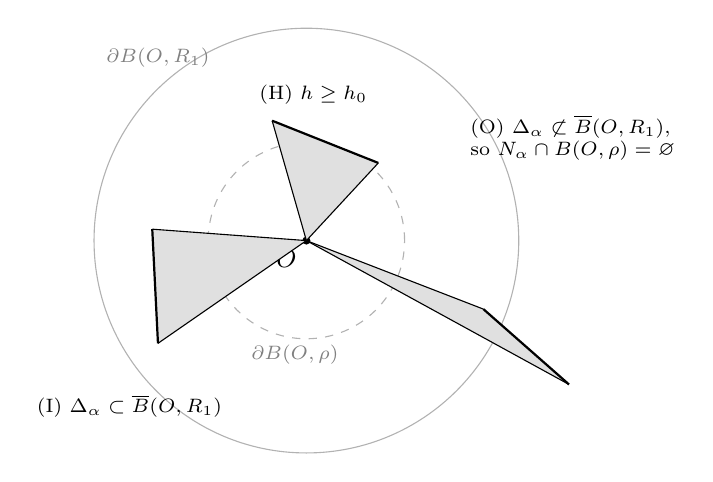
\begin{tikzpicture}[scale=1.45,>={Stealth[length=2mm]}]
  \coordinate (O) at (0,0);
  \draw[gray!60] (O) circle (1.86);
  \draw[gray!60,dashed] (O) circle (0.86);
  \fill (O) circle (1.0pt) node[below left,font=\small]{$O$};
  \node[gray,font=\scriptsize] at (-1.30,1.60) {$\partial B(O,R_{1})$};
  \node[gray,font=\scriptsize] at (-0.10,-1.00) {$\partial B(O,\rho)$};
  % (H) high triangle
  \fill[black!12] (O) -- (-0.30,1.05) -- (0.63,0.68) -- cycle;
  \draw[thick] (-0.30,1.05) -- (0.63,0.68);
  \draw (O) -- (-0.30,1.05); \draw (O) -- (0.63,0.68);
  \node[font=\scriptsize] at (0.06,1.28) {(H) $h\ge h_{0}$};
  % (I) confined triangle
  \fill[black!12] (O) -- (-1.35,0.10) -- (-1.30,-0.90) -- cycle;
  \draw[thick] (-1.35,0.10) -- (-1.30,-0.90);
  \draw (O) -- (-1.35,0.10); \draw (O) -- (-1.30,-0.90);
  \node[font=\scriptsize,align=center] at (-1.55,-1.45)
    {(I) $\Delta_{\alpha}\subset\overline B(O,R_{1})$};
  % (O) escaping triangle
  \fill[black!12] (O) -- (1.55,-0.60) -- (2.30,-1.26) -- cycle;
  \draw[thick] (1.55,-0.60) -- (2.30,-1.26);
  \draw (O) -- (1.55,-0.60); \draw (O) -- (2.30,-1.26);
  \node[font=\scriptsize,align=left,anchor=west] at (1.35,0.90)
    {(O) $\Delta_{\alpha}\not\subset\overline B(O,R_{1})$,\\
     so $N_{\alpha}\cap B(O,\rho)=\varnothing$};
\end{tikzpicture}
\caption{The radius trichotomy of Lemma~\ref{lem:trichotomy}, not to scale.
Either some chosen triangle is high (H), or a direction mass of at least $p\pi$
has its whole triangle confined to $\overline B(O,R_{1})$ (I), or a direction
mass of at least $(1-p)\pi$ escapes that disk (O). In case (O) the needle itself
must avoid the smaller ball $B(O,\rho)$, $\rho=R_{1}-1$, because a needle has
length $1$; this is the geometric input of Section~\ref{sec:caseII}.}
\label{fig:trichotomy}
\end{figure}

% ---------------------------------------------------------------------
\section{The confined-direction branch}\label{sec:caseI}

\emph{Input:} the height cap \eqref{eq:nohigh} and alternative (I) of
Lemma~\ref{lem:trichotomy}, that is, a direction mass of at least $p\pi$ whose
triangles lie in $\overline B(0,R_{1})$. \emph{Goal:} area strictly above
$\pi T$. \emph{Mechanism:} at each radius $r$, first arcs convert direction mass
into angular section mass; a same-centre dilation on the projective circle
controls the loss; polar slicing turns the angular sections into planar area
inside $\overline B(0,r_{0})$; and a strengthened form of Li's Lemma 2.5
converts that local area into total area. \emph{Output:}
Proposition~\ref{prop:caseI}.

Throughout this section we assume \eqref{eq:nohigh} and alternative (I).

\subsection{Canonical first arcs}

Normalise the support orientation of each chosen needle so that every signed
support height is nonnegative; this does not change the triangle
$\Delta_{\alpha}$, and under \eqref{eq:nohigh} the height lies in $[0,h_{0})$.

For each radius $r\in[h_{0},r_{0}]$ and each direction $\alpha$, the intersection
\[
  \Delta_{\alpha}\cap \partial B(0,r)
\]
consists of one or two closed polar arcs. We select the \emph{first arc}
deterministically: the longer component, with a fixed tie-breaking convention.
This is constructed data, not a selection hypothesis, and in particular no
continuity or measurability of $\alpha\mapsto$ first arc is claimed or used.

Write the selected arc of the direction $\alpha$ as a lifted interval
$[\ell_{\alpha},u_{\alpha}]$ with
\[
  t_{\alpha}=u_{\alpha}-\ell_{\alpha},\qquad
  x_{\alpha}=\tfrac12(\ell_{\alpha}+u_{\alpha}),\qquad
  w_{\alpha}=\tfrac12 t_{\alpha},
\]
and let $\Gamma_{\alpha}\subset\Tp$ denote its closed polar carrier. Put
\[
  J\Gamma_{\alpha}
  =\{\beta\in\Tp:\ \text{the selected first arc of }\beta
     \text{ is contained in }\Gamma_{\alpha}\}.
\]

\subsection{The dilation factor and endpoint containment}

For $r$ in the working range define
\begin{equation}\label{eq:gdef}
  g(r)=\max\left\{
    \frac{1+2r}{1-2r},\quad
    \frac{1+2r_{\lambda}}{1-2r_{\lambda}},\quad
    \frac{\pi}{\pi/2-\arctan(2r)}
  \right\},
\end{equation}
the three entries being the interior endpoint ratio, the frozen-radius ratio and
the large-angle ratio. Each entry is a loss incurred by one of the three
geometric regimes in which a competing direction can sit, and the argument must
pay the active maximum rather than a preferred branch. One has $g(r)>1$
throughout the range.

For $x\in\Tp$, $w\ge0$ and $g>1$ let $D_{g}(x,w)\subset\Tp$ be the centred
dilation of the arc of centre $x$ and radius $w$ by the factor $g$, with the
\emph{hybrid convention} that a source of radius $w=0$ is represented by the
closed singleton $\{x\}$ rather than by an open arc. The convention is essential:
an open arc of radius zero is empty, and the degenerate case does occur.

Before the containment itself we isolate the genuinely local step. It compares
one selected first arc with one competing direction, after rotating the chart so
that each end of the target span is an actual endpoint.

\begin{lemma}[local endpoint-contact gap]\label{lem:localcontact}
Let $r\in[h_{0},r_{0}]$, let $\alpha$ be a direction whose selected first arc has
been normalised to the span $[0,t]$ with $0<t<\pi$, and let $\beta$ be a
direction with $h(\beta)\in(0,h_{0}]$ whose triangle $\Delta_{\beta}$ has both
base endpoints in $\overline B(0,R_{1})$ and whose selected first arc is
contained in the normalised carrier. Write $\gamma$ for a lift of $\beta$ to the
chart. Then the two endpoint gaps satisfy
\[
  2\,\Phi_{\mathrm{up}}(\gamma,t)-t\ <\ g(r)\,t,
  \qquad
  2\,\Phi_{\mathrm{lo}}(\gamma,t)-t\ <\ g(r)\,t,
\]
where $\Phi_{\mathrm{up}}$ and $\Phi_{\mathrm{lo}}$ are the analytic lifts
obtained by rotating the upper, respectively lower, end of the chosen lift onto
the end of the target span. Consequently $\beta$ lies in the open centred
dilate $D_{g(r)}(t/2,t/2)$.
\end{lemma}

\begin{proof}
Rotate the chosen lift so that its upper endpoint sits at $t$, respectively its
lower endpoint at $0$; the statement is covariant under this rotation and the
two rotations give the two displayed gaps. The estimate then splits into four
geometric situations, of which only the last two are quantitative.

If the competing lift already reaches the far half of the chart, so that its
analytic angle is at most $t$, the bound is immediate from $g(r)>1$.

If the competing direction is controlled by a comparison height $\delta_{0}$
with $0<\delta_{0}<r$ and the target span is at least the endpoint phase
$\varphi(r,\delta_{0})$, then, on the quarter chart, the chart angle satisfies
$\sin\gamma\le\delta_{0}/r$ and the gap bound follows from monotonicity of
$\varphi$ in its height argument.

In the mixed situation the target span is exactly the endpoint phase and the
selected arc is the longer of the two components. Writing its span as
$\arcsin(h(\beta)/r)-\arctan(h(\beta)/b)$ with an effective base $b\ge\tfrac12$,
selectedness forces this span to be at most $t$, and monotonicity of
$\varphi(r,\cdot)$ then forces the physical height $h(\beta)$ to be at most the
comparison height, so that the analytic lift stays below the comparison circle.

In the remaining base-to-base situation both ends of the span are base
endpoints. With $\psi_{1}\le\psi_{2}$ the two ray angles, the single-ray chord
identity $\sin\psi_{1}\sin\psi_{2}=h(\beta)\sin(\psi_{2}-\psi_{1})$ together
with the endpoint norm bound $h(\beta)\le R_{1}\sin\psi_{1}$ --- which is where
$\beta\in\Ain(R_{1})$ is used --- gives the radius and height constraints that
close the gap.

The right-hand component of a reflected carrier is handled by the same four
cases applied to a projectively equivalent oriented lift, so no oriented angle
is ever confused with its antipode. Finally, if the resulting dilate has length
at least $\pi$ it saturates and equals $\Tp$, and if the height of $\beta$ is
zero the direction coincides with an endpoint of the span. Combining the two
gaps with the definition of a centred dilate places $\gamma$ in
$D_{g(r)}(t/2,t/2)$.
\end{proof}

\begin{proposition}[pointwise endpoint containment]\label{prop:endpoint}
Assume \eqref{eq:nohigh} and let $r\in[h_{0},r_{0}]$. For every direction $\alpha$,
\begin{equation}\label{eq:containment}
  \Ain(R_{1})\cap J\Gamma_{\alpha}
  \ \subset\ D_{g(r)}\bigl(x_{\alpha},w_{\alpha}\bigr).
\end{equation}
\end{proposition}

The restriction to $\Ain(R_{1})$ on the left of \eqref{eq:containment} is not
cosmetic: the argument uses that the base endpoints of the competing triangle lie
in $\overline B(0,R_{1})$, and the containment is false without that hypothesis.
The statement is also pointwise in $\alpha$ and in $r$; nothing is integrated
yet.

\begin{proof}
In the nondegenerate case $t_{\alpha}>0$ one first normalises the target arc to
$[0,t_{\alpha}]$ by rotating support angles; the statement is covariant under
this translation, and it carries $x_{\alpha}$ to $t_{\alpha}/2$ and
$w_{\alpha}$ to $t_{\alpha}/2$. If the dilated arc already has length $\ge\pi$
it is all of $\Tp$ and there is nothing to prove. Otherwise let $\beta$ lie in
the left-hand side. Since $\beta\in\Ain(R_{1})$ the base endpoints of
$\Delta_{\beta}$ lie in $\overline B(0,R_{1})$, and since
$\beta\in J\Gamma_{\alpha}$ its selected first arc lies in $\Gamma_{\alpha}$;
under \eqref{eq:nohigh} its height lies in $[0,h_{0}]$. If that height is
positive, Lemma~\ref{lem:localcontact} applies and places $\beta$ in
$D_{g(r)}(t_{\alpha}/2,t_{\alpha}/2)$, which is
$D_{g(r)}(x_{\alpha},w_{\alpha})$ after undoing the normalisation. If the height
is zero the first arc of $\beta$ degenerates to a point of $\Gamma_{\alpha}$,
which lies in the same dilate. The degenerate case $t_{\alpha}=0$ is separate: a
nondegenerate selected arc cannot be contained in a singleton carrier, so only
the direction $\alpha$ itself is involved, and it lies in the closed singleton by
construction.
\end{proof}

\begin{remark}[why the hypotheses cannot be weakened]\label{rem:counterexample}
Both hypotheses of Proposition~\ref{prop:endpoint} are necessary. An endpoint
dispatch that replaces the actual selected first arc by a raw exterior envelope,
or that drops the confined-class hypothesis $\beta\in\Ain(R_{1})$, admits an
explicit counterexample; the proposition must therefore be applied with the
actual first arc and with $\Ain(R_{1})$ in place.
\end{remark}

\begin{figure}[t]
\centering
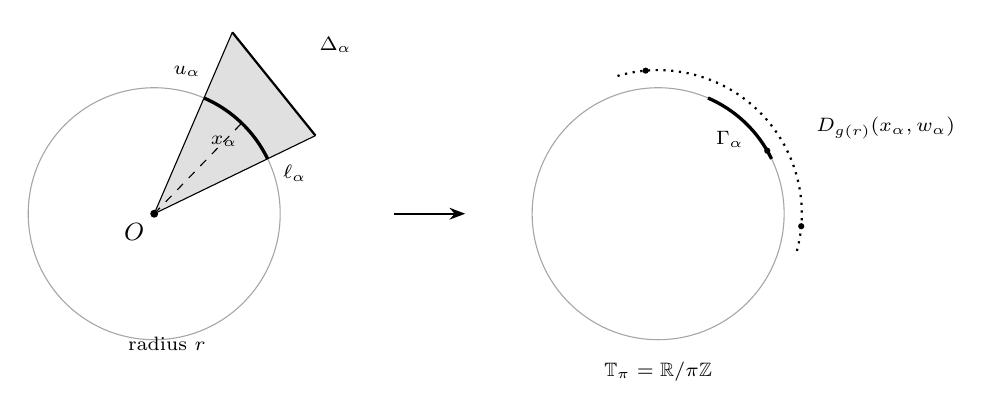
\begin{tikzpicture}[scale=1.0,>={Stealth[length=2mm]}]
  % ---- left: circle of radius r, triangle, first arc
  \begin{scope}[shift={(-3.5,0)},scale=1.6]
    \coordinate (O) at (0,0);
    \draw[gray!70] (O) circle (1);
    \fill (O) circle (0.9pt) node[below left,font=\small]{$O$};
    \fill[black!12] (O) -- (1.28,0.62) -- (0.62,1.44) -- cycle;
    \draw[thick] (1.28,0.62) -- (0.62,1.44);
    \draw (O) -- (1.28,0.62); \draw (O) -- (0.62,1.44);
    \draw[very thick] (25.8:1) arc (25.8:66.7:1);
    \node[font=\scriptsize] at (16:1.16) {$\ell_{\alpha}$};
    \node[font=\scriptsize] at (77:1.16) {$u_{\alpha}$};
    \node[font=\scriptsize] at (1.44,1.34) {$\Delta_{\alpha}$};
    \draw[dashed] (O) -- (46:1.0);
    \node[font=\scriptsize] at (46:0.80) {$x_{\alpha}$};
    \node[font=\scriptsize,below] at (0.10,-0.90) {radius $r$};
  \end{scope}
  % ---- right: projective circle with dilation
  \begin{scope}[shift={(2.9,0)},scale=1.6]
    \draw[gray!70] (0,0) circle (1);
    \node[font=\scriptsize] at (0,-1.25) {$\Tp=\R/\pi\Z$};
    \draw[very thick] (25.8:1) arc (25.8:66.7:1);
    \node[font=\scriptsize] at (46:0.82) {$\Gamma_{\alpha}$};
    \draw[thick,dotted] (-15:1.14) arc (-15:107:1.14);
    \node[font=\scriptsize,right] at (30:1.36) {$D_{g(r)}(x_{\alpha},w_{\alpha})$};
    \fill (30:1) circle (0.7pt);
    \fill (-5:1.14) circle (0.7pt);
    \fill (95:1.14) circle (0.7pt);
    \node[font=\scriptsize,align=left,anchor=west] at (-1.65,-0.72)
      {\phantom{x}};
  \end{scope}
  \draw[->,thick] (-0.45,0) -- (0.45,0);
\end{tikzpicture}
\caption{Confined-branch geometry. Left: at radius $r$, the triangle
$\Delta_{\alpha}$ meets the circle $\partial B(O,r)$ in one or two arcs; the
selected \emph{first arc} $[\ell_{\alpha},u_{\alpha}]$ has centre $x_{\alpha}$
and half-span $w_{\alpha}$. Right: on the projective circle $\Tp$, every
direction of the confined class $\Ain(R_{1})$ whose own first arc lies in the
carrier $\Gamma_{\alpha}$ is contained in the same-centre dilate
$D_{g(r)}(x_{\alpha},w_{\alpha})$ (Proposition~\ref{prop:endpoint}). Dilating an
arbitrary family about its own centres, rather than passing to a disjoint
subfamily, is what avoids a constant loss in the aggregate estimate
(Lemma~\ref{lem:dilation}).}
\label{fig:firstarc}
\end{figure}

\subsection{Same-centre dilation of an arbitrary arc family}

Proposition~\ref{prop:endpoint} is pointwise; to use it we must aggregate over
$\alpha$ without extracting a disjoint subfamily, since any such extraction costs
a constant factor. The following estimate is what makes that possible, and it is
one of the two places where the present argument departs from the earlier
circular-section proofs.

\begin{lemma}[same-centre dilation]\label{lem:dilation}
Let $\{(x_{i},w_{i})\}_{i\in\mathcal I}$ be an arbitrary family of centres
$x_{i}\in\Tp$ and radii $w_{i}\ge0$, indexed by an arbitrary set, and let $g>1$.
With the hybrid convention above,
\[
  \Lone\Bigl(\bigcup_{i\in\mathcal I}D_{g}(x_{i},w_{i})\Bigr)
  \ \le\ g\;\Lone\Bigl(\bigcup_{i\in\mathcal I}D_{1}(x_{i},w_{i})\Bigr).
\]
No disjointness, countability or measurability of the family is assumed.
\end{lemma}

\begin{proof}
Split the index set into $P=\{i:w_{i}>0\}$ and $N=\{i:w_{i}=0\}$, and put
\[
  U=\bigcup_{i\in P}D_{1}(x_{i},w_{i}),\qquad
  V=\bigcup_{i\in P}D_{g}(x_{i},w_{i}),\qquad
  Z=\{x_{i}:i\in N\},
\]
so that the source union is $U\cup Z$ and the dilated union is $V\cup Z$. Note
$U\subset V$ because $g\ge1$, and $U$ is open.

\emph{Positive radii.} We claim $\Lone(V)\le g\,\Lone(U)$. If $U=\Tp$ then also
$V=\Tp$ and the claim reads $\Lone(\Tp)\le g\,\Lone(\Tp)$, which holds. Otherwise
pick a point $\mathrm{cut}\in\Tp\setminus U$ and use it as a common cut: each
open arc $D_{1}(x_{i},w_{i})$ omits $\mathrm{cut}$, so it admits a lift to an
open interval contained in the fundamental interval
$(\mathrm{cut},\mathrm{cut}+\pi)$, and we fix one such lift for each $i\in P$.
Let $W\subset\R$ be the union of these lifted intervals. Being open in $\R$, $W$
is the disjoint union of at most countably many open interval components
$(a_{j},b_{j})$; assign to each $i\in P$ the component $j(i)$ containing its
lift. A same-centre dilation by $g$ of an interval contained in $(a_{j},b_{j})$
is contained in the dilation of $(a_{j},b_{j})$ about its own midpoint, whose
length is $g(b_{j}-a_{j})$. Hence, projecting back to $\Tp$ and using countable
subadditivity on the left and countable additivity of the disjoint components on
the right,
\[
  \Lone(V)\ \le\ \sum_{j}g\,(b_{j}-a_{j})
  \ =\ g\sum_{j}(b_{j}-a_{j})\ =\ g\,\Lone(U).
\]
The only lift of exact period length is the punctured circle, for which
$\Lone(U)=\Lone(\Tp)$ and the inequality is again immediate. No disjointness,
countability or measurability of the original family is used: only the
components of the open set $W$ are countable and disjoint, and that is automatic
on the line.

\emph{Zero radii.} The points of $Z$ are fixed by dilation, so they occur
unchanged on both sides. Carath\'eodory splitting by the measurable set $U$
gives $\Lone(U\cup Z)=\Lone(U)+\Lone(Z\setminus U)$, and since $U\subset V$,
\[
  \Lone(V\cup Z)\ \le\ \Lone(V)+\Lone(Z\setminus U)
  \ \le\ g\,\Lone(U)+g\,\Lone(Z\setminus U)
  \ =\ g\,\Lone(U\cup Z),
\]
each zero-radius point outside $U$ being charged exactly once. This is why the
hybrid convention is required: with the empty open arc of radius zero the source
union would lose $Z$ while the dilated union would not.
\end{proof}

\subsection{Aggregation and outer-measure polar slicing}

Every direction lies in its own class $J\Gamma_{\alpha}$. Hence
Proposition~\ref{prop:endpoint} yields, for each fixed $r$, a cover of the whole
confined class $\Ain(R_{1})$ by the dilated first-arc bases, and
Lemma~\ref{lem:dilation} bounds the outer length of that cover by $g(r)$ times
the outer length of the union of the undilated hybrid bases. The latter union
projects into the actual angular section at radius $r$ of $\Tri(E)$.
With the confined mass $\ge p\pi$ from alternative (I) this gives, for every
$r\in[h_{0},r_{0}]$, an angular section of outer size at least
\begin{equation}\label{eq:section}
  q(r)=\frac{\pi p}{g(r)} .
\end{equation}

It remains to convert a family of angular section bounds into planar area. Since
$E$ is not assumed measurable, this step needs an outer-measure statement.

\begin{lemma}[polar slicing for outer measure]\label{lem:polar}
Let $S\subset\R^{2}$ and let $0<r_{1}<r_{2}$. Suppose that for every
$r\in[r_{1},r_{2}]$ the angular section
$\{\theta:\ r e(\theta)\in S\}$ has one-dimensional outer measure at least
$q(r)$, where $q$ is measurable on $[r_{1},r_{2}]$. Then
\[
  \Lout\bigl(S\cap\overline B(0,r_{2})\bigr)
  \ \ge\ \int_{r_{1}}^{r_{2}} r\,q(r)\,dr .
\]
\end{lemma}

\begin{proof}
Fix $\epsilon>0$. Let $U\supset S\cap\overline B(0,r_{2})$ be open with
$|U|\le\Lout(S\cap\overline B(0,r_{2}))+\epsilon$; such $U$ exists by the
definition of Lebesgue outer measure through open covers. The set $U$ is
measurable, so the polar coordinate formula applies to it and gives
$|U|=\int_{0}^{\infty}r\,\lambda_{1}(U_{r})\,dr$, where $U_{r}$ is the angular
section of $U$ at radius $r$ and $\lambda_{1}$ is angular Lebesgue measure. For
$r\in[r_{1},r_{2}]$ the section $U_{r}$ contains the section of $S$, hence
$\lambda_{1}(U_{r})\ge q(r)$ by monotonicity of outer measure and measurability
of $U_{r}$. Therefore
$|U|\ge\int_{r_{1}}^{r_{2}}r\,q(r)\,dr$, and letting $\epsilon\downarrow0$
finishes the proof. No measurability of $S$ or of its sections is used.
\end{proof}

Applying Lemma~\ref{lem:polar} to $S=\Tri(E)$ with the sections
\eqref{eq:section} on $[h_{0},r_{0}]$ gives
\begin{equation}\label{eq:radialint}
  \Lout\bigl(\Tri(E)\cap \overline B(0,r_{0})\bigr)
  \ \ge\ \pi p\int_{h_{0}}^{r_{0}}\frac{r}{g(r)}\,dr .
\end{equation}
The bounding circle is null, so the same bound holds for the open disk.

We stress that \eqref{eq:radialint} is an \emph{aggregate} statement. At no
point is a single first arc asserted to carry direction mass $p\pi$; and the
intersection with $\Ain(R_{1})$ in \eqref{eq:containment} is equally essential.

\subsection{The radial integral}

The integral in \eqref{eq:radialint} has an elementary integrand with one
transcendental entry, and we replace it by an exact rational lower bound.

\begin{proposition}[radial integral certificate]\label{prop:integral}
With the cut points
\[
  L=\frac{9}{40}=0.225,\qquad U=\frac{2353}{10000}=0.2353,
\]
one bounds $g$ above by the frozen branch on $[h_{0},L]$, by the constant
$g_{\mathrm{int}}(U)=(1+2U)/(1-2U)$ on $[L,U]$, and by the exact interior ratio
$(1+2r)/(1-2r)$ on $[U,r_{0}]$, so that
\[
  \int_{h_{0}}^{r_{0}}\frac{r}{g(r)}\,dr
  \ \ge\
  \frac{L^{2}-h_{0}^{2}}{2g_{\mathrm{frozen}}}
  +\frac{U^{2}-L^{2}}{2g_{\mathrm{int}}(U)}
  +\int_{U}^{r_{0}}\frac{r(1-2r)}{1+2r}\,dr ,
\]
where $g_{\mathrm{frozen}}=(1+2r_{\lambda})/(1-2r_{\lambda})$. Evaluating the
last integral by its primitive
\[
  -\frac{r^{2}}{2}+r-\frac12\log(1+2r)
\]
and bounding the logarithmic increment from above through the odd-power series in
$z=x/(x+2)$ with an explicit geometric tail yields the exact rational number
\begin{equation}\label{eq:Istar}
  \Istar=\frac{22793357350571006116275623711763}
              {1064174925446566790615478200000000}
  =0.0214188\ldots
\end{equation}
and the chain
\begin{equation}\label{eq:Istarchain}
  \Istar\ \le\ C_{\mathrm{cut}}\ \le\ \int_{h_{0}}^{r_{0}}\frac{r}{g(r)}\,dr ,
\end{equation}
where $C_{\mathrm{cut}}$ denotes the three-term cut expression displayed above.
\end{proposition}

\begin{proof}
The cut points are chosen strictly inside the two intervals on which the active
entry of the maximum \eqref{eq:gdef} changes, so on each of the three
subintervals the displayed majorant dominates $g$; since $r/g(r)$ is decreasing
in $g$, the integral is bounded below termwise. The first two terms are
elementary. For the third, the displayed primitive is exact, and the logarithmic
increment is bounded above by the truncated odd-power series in $z$ together
with an explicit geometric tail, which is a rational upper bound. This proves
the second inequality of \eqref{eq:Istarchain}; the first is an exact comparison
of rational numbers.
\end{proof}

\begin{remark}[normalisation and cut points]\label{rem:noThird}
$\Istar$ is a lower bound for the \emph{full} integral in
\eqref{eq:Istarchain}; there is no additional factor $1/3$ anywhere in the
normalisation, and multiplying $\Istar$ by three would state a false inequality.
The cut points $0.225$ and $0.2353$ are safe rational values, not the actual
crossings of the three entries of \eqref{eq:gdef}, which are approximately
$0.2250516$ and $0.2352988$; and $\Istar$ is a stored rational lower bound for
the cut expression, not an evaluation of it.
\end{remark}

\subsection{Local-to-global conversion}

Estimate \eqref{eq:radialint} bounds the area inside the working disk
$B(0,r_{0})$ only, whereas the theorem is about the whole set. The following
strengthening of Li's Lemma~2.5 supplies the conversion, and it is the reason
the local radial mass computed above is enough.

\begin{proposition}[strong Lemma 2.5, fixed parameters]\label{prop:li25}
Let the chosen family satisfy $|h(\alpha)|\le h_{0}$ for all $\alpha$, and suppose
\[
  s_{0}\ \le\ \Lout\bigl(\Tri(E)\cap B(0,r_{0})\bigr).
\]
Then, with $f_{0}$ and $k$ as in \eqref{eq:fkdef},
\[
  \frac{\pi}{4}f_{0}+k\,s_{0}\ \le\ \Lout(\Tri(E)).
\]
\end{proposition}

\begin{proof}
For each $\epsilon>0$ one runs a greedy selection on the direction circle whose
deletion radius is set by a fixed rule from the height of the selected
triangle. The selected exterior pieces are pairwise disjoint by the
angular separation geometry, and their exterior area payments are summed; the
undeleted zero-height directions generate a radial sector, which supplies the
term $\tfrac{\pi}{4}f_{0}$, while the coefficient $k$ discounts the part of the
inner mass $s_{0}$ that the exterior payments would otherwise double count. The
bookkeeping is carried out in $[0,\infty]$ throughout, so no step converts
$+\infty$ to a real number. Concavity of
$u\mapsto\arcsin\bigl((1-\epsilon)\sin u\bigr)$ produces the factor
$2\arcsin(1-\epsilon)/\pi$, and letting $\epsilon\to0$ gives the stated
inequality. The height cap $|h|\le a$ is essential: it places the selected
triangles in the range where the exterior estimate applies.
\end{proof}

\subsection{The confined-branch bound}

\begin{proposition}[confined branch]\label{prop:caseI}
Under \eqref{eq:nohigh} and alternative (I),
\[
  \Lout(E)\ \ge\ \pi\Bigl(p\,k\,\Istar+\frac{f_{0}}{4}\Bigr)\ >\ \pi T .
\]
\end{proposition}

\begin{proof}
Apply Proposition~\ref{prop:li25} with $s_{0}=\pi p\Istar$, which is legitimate
by \eqref{eq:radialint} and Proposition~\ref{prop:integral}, and use
$\Tri(E)\subset E$ together with the measure-preserving centring of
coordinates. The strict inequality is the exact rational identity
\[
  p\,k\,\Istar+\frac{f_{0}}{4}-T
  =\frac{139158989937085958631189100903645702101397}
        {664352167944649011863150962260700000000000000000}
  \ >\ 0,
\]
whose value is $2.0946\ldots\times10^{-7}$.
\end{proof}

In the notation of \eqref{eq:designbounds} this is the branch
$\mathrm{I}=A_{0}+pX_{*}$ with $A_{0}=f_{0}/4$ and the certified surrogate
$X_{*}=k\Istar$ of \eqref{eq:Xsur}. This supplies one of the two alternatives left open by
Lemma~\ref{lem:trichotomy}.

% ---------------------------------------------------------------------
\section{The escaping-direction branch}\label{sec:caseII}

\emph{Input:} the height cap \eqref{eq:nohigh} and alternative (O) of
Lemma~\ref{lem:trichotomy}, that is, a direction mass of at least $(1-p)\pi$
whose triangles leave $\overline B(0,R_{1})$. \emph{Goal:} area strictly above
$\pi T$. \emph{Mechanism:} escaping needles avoid a fixed inner ball, so each
selected triangle can pay for the direction mass deleted around it; a greedy
selection whose deletion radius is set by a \emph{fixed rule} from the height of
the selected triangle keeps the selected triangles disjoint, and the directions
that survive all deletions sweep a radial fan.
\emph{Output:} Proposition~\ref{prop:caseII}.

Throughout this section we assume \eqref{eq:nohigh} and alternative (O).

\subsection{The forbidden inner ball}

\begin{lemma}[escaping needles avoid $B(0,\rho)$]\label{lem:outside}
If $\alpha\in\Aout(R_{1})$ then $N_{\alpha}\cap B(0,\rho)=\varnothing$, where
$\rho=R_{1}-1$.
\end{lemma}

\begin{proof}
Suppose some point of the needle lay in $B(0,\rho)$. The needle has length $1$,
so all of it would lie in $B(0,\rho+1)=B(0,R_{1})$, and then the triangle
$\Delta_{\alpha}$, being the union of the segments from $0$ to points of
$N_{\alpha}$, would lie in $\overline B(0,R_{1})$ as well --- contradicting
$\alpha\in\Aout(R_{1})$.
\end{proof}

Thus the escaping branch does not need a separately postulated
``outside-ball'' hypothesis: it is forced by the radius class.

\subsection{The payment inequality}

The selection below deletes direction mass around each selected triangle, and
each deletion must be paid for by the area of that triangle. We therefore fix
the weights before describing the selection. Let
\[
  \epsdel=10^{-10},\qquad m=1-\epsdel,
\]
and, for a needle of height $\delta$, define the angular half-width and the two
weights
\begin{equation}\label{eq:weights}
  H(\delta)=\arcsin\frac{\delta}{m\rho},
  \qquad
  c=\frac{h_{0}}{2\arcsin(h_{0}/\rho)},
  \qquad
  \kappa=\frac{2\arcsin(m)}{\pi} .
\end{equation}
Under \eqref{eq:nohigh} one has $0\le\delta<h_{0}<m\rho$ by the domain condition
$h_{0}<(1-\epsdel)\rho$ of \eqref{eq:domain}, so $H(\delta)$ is defined.
Concavity of $u\mapsto\arcsin(m\sin u)$ together with the single-triangle area
bound of Lemma~\ref{lem:triangle} gives the \emph{payment inequality}
\begin{equation}\label{eq:payment}
  c\,\kappa\,H(\delta)\ \le\ \frac{\delta}{2}
  =\operatorname{area}(\Delta_{\alpha}),
\end{equation}
which says exactly that a triangle of height $\delta$ can afford an angular
deletion of half-width $H(\delta)$ at the fixed rate $c\kappa$.

\subsection{Angular shadows and disjointness}

Lemma~\ref{lem:outside} alone does not make two triangles disjoint; what it
supplies is that each escaping needle lives outside $B(0,\rho)$, and therefore
casts an angular \emph{shadow} at the origin of half-width
$\arcsin(\delta/\rho)$, where $\delta$ is its height. Two triangles whose
shadows do not overlap cannot meet.

\begin{lemma}[shadow separation]\label{lem:shadow}
Let $N_{1},N_{2}$ be unit needles with $N_{i}\cap B(0,\rho)=\varnothing$, of
heights $\delta_{1},\delta_{2}\in(0,\rho)$ and projective directions
$\theta_{1},\theta_{2}$. If
\[
  \operatorname{dist}_{\Tp}(\theta_{1},\theta_{2})
  \ >\ \arcsin\frac{\delta_{1}}{\rho}+\arcsin\frac{\delta_{2}}{\rho},
\]
then the open triangles $\operatorname{int}\conv(\{0\}\cup N_{1})$ and
$\operatorname{int}\conv(\{0\}\cup N_{2})$ are disjoint.
\end{lemma}

\begin{proof}
Let $x$ be an interior point of $\conv(\{0\}\cup N_{i})$ and let $\phi$ be the
angle between the ray $[0,x)$ and the direction $\theta_{i}$. The ray through
$x$ meets the relative interior of $N_i$ at a point $y$. In fact $|y|>\rho$:
if $|y|=\rho$, then because $\delta_i<\rho$ the line of the needle crosses the
open ball immediately on one side of $y$, and the fact that $y$ is interior to
the segment would force $N_i\cap B(0,\rho)\ne\varnothing$. Since the distance
from the origin to the line of $N_i$ is $\delta_i$, it follows that
$\sin\phi=\delta_i/|y|<\delta_i/\rho$. Thus every direction occurring in the
open triangle lies in the open projective ball
$B_{\Tp}(\theta_i,\arcsin(\delta_i/\rho))$. The two shadows are therefore
contained in the projective balls $B_{\Tp}(\theta_{i},\arcsin(\delta_{i}/\rho))$,
which are disjoint under the displayed separation hypothesis; two sets of
directions that are disjoint cannot be realised by a common point other than the
origin, which is not interior to either triangle.
\end{proof}

\subsection{Adaptive-radius deletion and the budget inequalities}

The selection is run with a deletion radius set by a fixed rule from the height
of the selected triangle; the radius used at stage $j$ is $2H_{j}$, so it varies
from stage to stage but is never chosen adaptively against the geometry. At
stage $j$, choose a strict $m$-approximate maximiser $\theta_{j}$ of the heights
among the surviving directions, write $\delta_{j}=h(\theta_{j})$ and
$H_{j}=H(\delta_{j})$, and delete from the surviving set the projective metric
ball
\[
  B_{\Tp}(\theta_{j},2H_{j}).
\]
Deleting this ball costs at most $4H_{j}$ of direction mass. If a later centre
$\theta_{n}$ survives stage $j$, then $\operatorname{dist}(\theta_{j},\theta_{n})\ge2H_{j}$,
while approximate maximality gives
\[
  \arcsin\frac{\delta_{j}}{\rho}<H_{j},
  \qquad
  \arcsin\frac{\delta_{n}}{\rho}<H_{j}\qquad (j<n),
\]
whence
\[
  \arcsin\frac{\delta_{j}}{\rho}+\arcsin\frac{\delta_{n}}{\rho}
  <\operatorname{dist}(\theta_{j},\theta_{n}).
\]
Lemma~\ref{lem:outside} makes Lemma~\ref{lem:shadow} applicable to the selected
needles, and this angular separation is exactly its hypothesis; hence the
selected open triangles are pairwise disjoint. Note that only the two displayed
strict inequalities are used: the monotonicity $H_{n}<H_{j}$ for $j<n$ is false
in general and is never invoked.

\begin{proposition}[deletion budget]\label{prop:budget}
Let $L$ be the initial direction mass under consideration, $R$ the residual mass
after all deletions, $B=\sum_{j}4H_{j}$ the total deletion cost, $b$ the total
area of the selected triangles, and $M=\Lout(E)$; these five symbols are local to
this subsection. Then
\begin{equation}\label{eq:caseIIthree}
  L\le R+B,\qquad \frac{c\kappa}{4}B\le b,\qquad
  \frac{\rho^{2}}{2}R+b\le M ,
\end{equation}
and consequently
\begin{equation}\label{eq:caseIImain}
  \frac{c\kappa}{4}\,L\ \le\ M .
\end{equation}
\end{proposition}

\begin{proof}
The first inequality is subadditivity of outer measure on the direction circle:
every direction of the initial class is either deleted at some stage or survives
all stages. For the second, \eqref{eq:payment} gives
$c\kappa H_{j}\le\operatorname{area}(\Delta_{\theta_{j}})$ at every stage, and
summing over the disjoint selected triangles yields
$\tfrac{c\kappa}{4}B=\sum_{j}c\kappa H_{j}\le b$. The third combines the disjointness of the
selected triangles with the residual radial fan: the residual directions have
zero height, and by Lemma~\ref{lem:outside} their needles avoid $B(0,\rho)$, so
they sweep a sector of radius $\rho$ and angular mass $R$, of area
$\rho^{2}R/2$, disjoint from the selected triangles.

The recursion has a genuine finite-stop alternative as well as an infinite one.
At a finite stop, all residual heights are zero. In the infinite case, either
$B<\infty$, in which case summability forces the residual heights to zero, or
$B=\infty$, in which case the positive selected-area payments already force
$M=\infty$ and \eqref{eq:caseIImain} holds trivially. In the remaining case,
$c\kappa/4\le\rho^{2}/2$ --- which is where $\rho>\tfrac12$ from
\eqref{eq:domain} is used --- lets us eliminate $R$ and $b$ from
\eqref{eq:caseIIthree}:
\[
  \frac{c\kappa}{4}L\le\frac{c\kappa}{4}R+\frac{c\kappa}{4}B
  \le\frac{\rho^{2}}{2}R+b\le M . \qedhere
\]
\end{proof}

\subsection{The escaping-branch bound}

\begin{proposition}[escaping branch]\label{prop:caseII}
Under \eqref{eq:nohigh} and alternative (O),
\[
  \Lout(E)\ \ge\ \frac{c\kappa}{4}(1-p)\pi\ >\ \pi T .
\]
\end{proposition}

\begin{proof}
Alternative (O) gives $L\ge(1-p)\pi$ in \eqref{eq:caseIImain}. The strict
comparison is the exact inequality
\[
  \frac{T}{1-p}<\frac{c\kappa}{4},
\]
proved from the rational lower bound $\kappa>99999/100000$ and a certified
rational enclosure of the inverse-sine ratio in \eqref{eq:weights};
numerically $c\kappa/4=0.1069578\ldots$ while $T/(1-p)=0.1069545\ldots$
\end{proof}

In the notation of \eqref{eq:designbounds} this is the branch
$\mathrm{O}=(1-p)Y$ carrying the fixed loss $\kappa$ of
Remark~\ref{rem:kappaloss}: the limiting coefficient $c/4$ suggested by an
informal reading is \emph{not} used, and no limit $\epsdel\to0$ is taken
\emph{in this branch}. The confined branch is different: the local-to-global
conversion of Proposition~\ref{prop:li25} does pass to the limit in its own
auxiliary parameter, and legitimately so, because there the limit is taken
inside an inequality that holds for every positive value of that parameter.
This supplies the second of the two alternatives left open by
Lemma~\ref{lem:trichotomy}.

% ---------------------------------------------------------------------
\section{Additive confined/exterior refinement}\label{sec:additive}

\emph{Input:} the same arbitrary chosen triangle family as in
Part~\ref{part:lower}, together with the confined machinery of
Section~\ref{sec:caseI} used as a quoted black box. \emph{Goal:} a universal
bound with a strictly larger constant than the baseline
Theorem~\ref{thm:lower}. \emph{Mechanism:} stop splitting the direction circle
by a mass proportion, and split the \emph{plane} instead. A fixed closed ball
separates the two payments: confined directions are charged only inside it,
escaping directions only outside it, and the two charges are added by
Carath\'eodory splitting rather than compared in a minimax. \emph{Output:}
Proposition~\ref{prop:annbudget}, Proposition~\ref{prop:annconfined} and
Theorem~\ref{thm:annular}.

Sections~\ref{sec:trichotomy}--\ref{sec:caseII} remain in force as written: the
baseline route and its constant $100\pi/5599$ are not modified, not
reparametrised and not retracted, and Theorem~\ref{thm:lower} continues to be
proved exactly as above. The present section and
Section~\ref{sec:annbudget} add a \emph{second, independent} route to a larger
constant, and they reuse from the baseline development only those statements
that are explicitly quoted below.

\subsection{Why the two contributions add}\label{sec:addidea}

In the baseline route the confined and the escaping class compete. Alternative
(I) and alternative (O) of Lemma~\ref{lem:trichotomy} are mutually exclusive
readings of one and the same direction circle, a proportion $p$ has to be
chosen in advance, and the proved constant is the value of the minimax
described by Lemma~\ref{lem:balance}. Both branches then charge the whole set
$E$, which is why neither may charge what the other already charged: the
local-to-global conversion of Proposition~\ref{prop:li25} exists precisely to
make the confined branch's local mass into a global bound, and it pays for that
with the coefficient $k<1$ and with a fixed exterior tax.

The refinement removes the competition. Fix a radius $\hat r_{0}$ and split the
plane by the \emph{closed} ball $\overline B(0,\hat r_{0})$, which is
measurable even though $E$ is not. Carath\'eodory splitting is then an exact
identity for the outer measure of an arbitrary set,
\begin{equation}\label{eq:annsplit}
  \Lout(E)
  =\Lout\bigl(E\cap\overline B(0,\hat r_{0})\bigr)
  +\Lout\bigl(E\setminus\overline B(0,\hat r_{0})\bigr),
\end{equation}
and the two summands may be estimated by two arguments that never look at the
same region of the plane. The confined directions are charged inside: their
triangles produce circular sections at every radius $r\in[\hat h_{0},\hat
r_{0}]$, and the radial integral of those sections is an area \emph{inside} the
ball. The escaping directions are charged outside: an escaping needle avoids
the ball $B(0,\hat\rho)$ with $\hat\rho>\hat r_{0}$, so the part of its
triangle lying outside $\overline B(0,\hat r_{0})$ is nonempty and can be
estimated from below. No direction is charged twice, and no mass proportion is
needed: writing $L_{\mathrm{in}}$ and $L_{\mathrm{out}}$ for the direction
masses of the confined and the escaping class, all that is used about them is
the subadditivity bound
\begin{equation}\label{eq:annmass}
  \pi=\Lone(\Tp)\ \le\ L_{\mathrm{in}}+L_{\mathrm{out}} ,
\end{equation}
which needs no measurability because the two classes are literal complements.
Consequently, if the confined branch produces the coefficient $\hat I$ and the
escaping branch the coefficient $\hat C_{\mathrm{out}}$, then
\eqref{eq:annsplit} and \eqref{eq:annmass} give
\[
  \Lout(E)\ \ge\ \hat I\,L_{\mathrm{in}}+\hat C_{\mathrm{out}}L_{\mathrm{out}}
  \ \ge\ \min\{\hat I,\hat C_{\mathrm{out}}\}\,\bigl(L_{\mathrm{in}}+L_{\mathrm{out}}\bigr)
  \ \ge\ \pi\min\{\hat I,\hat C_{\mathrm{out}}\},
\]
with no minimax, no balance lemma and no proportion $p$ anywhere.

Three things must be arranged for this to be more than bookkeeping, and they
are the content of the two sections.

\begin{itemize}
  \item The confined branch must stay inside the ball. It therefore uses only
    the \emph{raw} radial integral $\hat I=\int_{\hat h_{0}}^{\hat r_{0}}r/\hat
    g(r)\,dr$ of \eqref{eq:radialint}, and it deliberately does \emph{not} use
    the local-to-global conversion of Proposition~\ref{prop:li25}; the
    coefficient $k$ and the additive term $f_{0}/4$ disappear from the
    refinement together with the double-counting problem they were solving.
  \item The escaping branch must stay outside the ball. Each selected triangle
    is charged only through $\Delta\setminus\overline B(0,\hat r_{0})$, and the
    directions that survive every deletion are charged only through the
    annulus $\hat r_{0}<|x|\le\hat\rho$ swept by their radial fan.
  \item The escaping payment must be large enough \emph{without} the
    proportion $p$. This is where the geometry has to be sharpened: the
    classical estimate treats the angular shadow of an escaping needle as
    symmetric about its direction, of full width $2\arcsin(\delta/\hat\rho)$,
    whereas a unit segment that avoids a disc cannot straddle it, so the
    shadow is one-sided (Lemma~\ref{lem:annonesided}) and the sector subtracted
    from the triangle is smaller by a factor of slightly more than two
    (Lemma~\ref{lem:annwidth}).
\end{itemize}

Before any numeral, the four quantities that the refinement has to compare are
these. With $\hat h_{0}$ the height threshold, $\hat g$ the dilation loss of
\eqref{eq:gdef} evaluated at the refinement parameters, $\hat\rho$ the exterior
ball radius, $\hat r_{0}$ the splitting radius, $m=1-\epsdel$ the fixed greedy
tolerance and $\hat H(\delta)=\arcsin\bigl(\delta/(m\hat\rho)\bigr)$ the
weighted angular half-width, put
\begin{equation}\label{eq:annsymbolic}
  \hat{\mathrm{H}}=\frac{\hat h_{0}}{2\pi},
  \qquad
  \hat I=\int_{\hat h_{0}}^{\hat r_{0}}\frac{r}{\hat g(r)}\,dr,
  \qquad
  \frac{\hat C_{\mathrm{ext}}}{4}
  =\frac{1}{4}\left(\frac{\hat h_{0}}{2\hat H(\hat h_{0})}
    -\frac{m\hat r_{0}^{2}}{2}\right),
  \qquad
  \hat C_{\mathrm{fan}}=\frac{\hat\rho^{2}-\hat r_{0}^{2}}{2}.
\end{equation}
The first is the high branch, the second the confined branch, the third the
rate at which one selected escaping triangle pays for the direction mass
deleted around it, and the fourth the rate at which the residual fan pays for
the mass that is never deleted. The theorem of Section~\ref{sec:annbudget} is
that the minimum of the four is a lower bound for $\Lout(E)/\pi$; the tuple
below is chosen so that this minimum exceeds $\hat T=131/6250$.

\subsection{Parameters for the refinement}\label{sec:annparameters}

All symbols of the refinement carry a hat, and they are independent of the
baseline constants \eqref{eq:params}, which keep their unhatted names
throughout.

\paragraph{Rational data.} Fix
\begin{equation}\label{eq:annparams}
  \hat h_{0}=\frac{13177}{100000},\quad
  \hat r_{\lambda}=\frac{10227}{50000},\quad
  \hat r_{0}=\frac{999}{2000},\quad
  \epsdel=10^{-10},\quad m=1-\epsdel,
\end{equation}
and the target $\hat T=\dfrac{131}{6250}$. The derived quantities are those of
\eqref{eq:lambdadef}--\eqref{eq:R1} evaluated at the hatted data:
\begin{equation}\label{eq:annderived}
  \hat\lambda=\frac{\hat r_{0}-\hat r_{\lambda}}{\hat r_{0}-\hat h_{0}}
  =\frac{29496}{36773},
  \qquad
  \hat Q=4\hat r_{\lambda}^{2}(1+\hat h_{0}^{2})-\hat h_{0}^{2},
  \qquad
  \hat d=\frac{\hat h_{0}\bigl(1-\sqrt{\hat Q}\bigr)}{2(1+\hat h_{0}^{2})},
\end{equation}
\begin{equation}\label{eq:annR1}
  \hat R_{1}=\frac{\sqrt{1+4\hat d^{2}}}{1-2\sqrt{\hat r_{\lambda}^{2}-\hat d^{2}}},
  \qquad
  \hat\rho=\hat R_{1}-1 ,
\end{equation}
and $\hat g$ is the function \eqref{eq:gdef} with $r_{\lambda}$ replaced by
$\hat r_{\lambda}$. The weights and the exterior coefficients are
\begin{equation}\label{eq:annweights}
  \hat H(\delta)=\arcsin\frac{\delta}{m\hat\rho}\quad(0\le\delta\le\hat h_{0}),
  \qquad
  \hat C_{\mathrm{ext}}=\frac{\hat h_{0}}{2\hat H(\hat h_{0})}
    -\frac{m\,\hat r_{0}^{2}}{2},
\end{equation}
\begin{equation}\label{eq:annCout}
  \hat C_{\mathrm{fan}}=\frac{\hat\rho^{2}-\hat r_{0}^{2}}{2},
  \qquad
  \hat C_{\mathrm{out}}
  =\min\Bigl\{\frac{\hat C_{\mathrm{ext}}}{4},\ \hat C_{\mathrm{fan}}\Bigr\}.
\end{equation}

\paragraph{Domain conditions.} The refinement needs
\begin{equation}\label{eq:anndomain}
\begin{gathered}
  0<\hat h_{0}\le\hat r_{\lambda}\le\hat r_{0}<\tfrac12,\qquad
  \hat r_{0}\ge\tfrac{3}{20},\qquad
  \hat\lambda\hat h_{0}+(1-\hat\lambda)\hat r_{0}=\hat r_{\lambda},\\
  0\le\hat Q<1,\qquad 0<\hat d<\tfrac{\hat h_{0}}{2},\qquad
  \hat r_{\lambda}^{2}-\hat d^{2}\ge0,\qquad
  1-2\sqrt{\hat r_{\lambda}^{2}-\hat d^{2}}>0,\\
  \hat\rho>\hat r_{0},\qquad \hat h_{0}<m\hat\rho,\qquad
  0<\frac{\hat h_{0}}{\hat\rho}<1,\qquad
  0<\frac{\hat h_{0}}{m\hat\rho}<1 .
\end{gathered}
\end{equation}
These are verified, not assumed; the enclosures are recorded in
Appendix~\ref{app:constants}. Two conditions of the baseline domain
\eqref{eq:domain} are conspicuously absent. The refinement needs neither
$\hat\rho>\tfrac12$ nor $\hat\rho\le1$, because the exterior coefficients are
combined by the explicit minimum \eqref{eq:annCout} rather than by the
comparison $c\kappa/4\le\rho^{2}/2$ used in Proposition~\ref{prop:budget}; and
the condition $\hat\rho>\hat r_{0}$ replaces $\rho>h_{0}$, since the splitting
radius, not the height threshold, is what has to sit inside the forbidden ball.

\begin{remark}[what the exterior branch no longer carries]\label{rem:annnokappa}
The fixed loss $\kappa=2\arcsin(m)/\pi$ of Remark~\ref{rem:kappaloss} does not
appear anywhere in the refinement. The tolerance $m$ is absorbed once and for
all into the weight $\hat H$ and hence into $\hat C_{\mathrm{ext}}$; see
Remark~\ref{rem:annconcavity}. No limit $\epsdel\to0$ is taken in either
branch of the refinement.
\end{remark}

\begin{remark}[the frozen entry is inactive at this tuple]\label{rem:annfrozen}
For the data \eqref{eq:annparams} the frozen entry
$(1+2\hat r_{\lambda})/(1-2\hat r_{\lambda})=35227/14773=2.38455\ldots$ of
$\hat g$ is dominated on all of $[\hat h_{0},\hat r_{0}]$ by the increasing
large-angle entry, whose value already at $r=\hat h_{0}$ is
$2.392472\ldots$. The maximum defining $\hat g$ therefore switches exactly
once, at $r=0.2352988\ldots$, between the large-angle and the interior entry.
This changes no proof --- $\hat g$ is always the full maximum of the three
entries --- but it does mean that $\hat I$ does not depend on $\hat
r_{\lambda}$ for this tuple, and that the three-piece cut of
Proposition~\ref{prop:integral} is not the right decomposition here; the
two-segment certificate actually used is described in
Appendix~\ref{app:constants}. The parameter $\hat r_{\lambda}$ enters the
refinement only through $\hat Q,\hat d,\hat R_{1},\hat\rho$.
\end{remark}

\begin{remark}[status and provenance of the refinement tuple]\label{rem:annprov}
The chronology is the same as for \eqref{eq:params}, and so are the
non-claims. A numerical scout of the family
\eqref{eq:annsymbolic} exhibits a basin in which the four coefficients are
simultaneously large; its reported optimum sits on the unattained boundary
$\hat r_{0}\to\tfrac12$, and \eqref{eq:annparams} is a deliberate rational
retreat from it, frozen before any of the estimates below were proved. An
interval certificate in outward-rounded Arb arithmetic then verifies
\eqref{eq:anndomain} and the four gates of \eqref{eq:anngates} for that frozen
tuple; this is \emph{evidence}, at the level described in
Section~\ref{sec:evidence}, and it is consumed neither by the Lean proof nor by
the exact-rational proof of this manuscript. It does discharge Hypotheses B
and C of the accompanying paper-level proof note, which is a conditional prose
argument and is not machine checked; that dependency must not be conflated with
the kernel-checked chain. The formal development reproves every domain
condition, every gate and all of the geometry from scratch in exact rational and
squared-rational arithmetic (Appendix~\ref{app:formalization}). We claim no optimality of
\eqref{eq:annparams}, no uniqueness, and no completed search of the legal
domain \eqref{eq:anndomain}; we do not claim that $\hat T=131/6250$ is the
largest target this witness supports.
\end{remark}

\subsection{One-sided annular triangle geometry}\label{sec:anngeom}

Escaping needles avoid an inner ball, exactly as in the baseline route:
Lemma~\ref{lem:outside}, whose proof uses nothing but the unit length of the
needle and star-shapedness, applies verbatim with $R_{1}$ replaced by
$\hat R_{1}$ and gives
\begin{equation}\label{eq:annoutside}
  \alpha\in\Aout(\hat R_{1})\ \Longrightarrow\
  N_{\alpha}\cap B(0,\hat\rho)=\varnothing,
  \qquad \hat\rho=\hat R_{1}-1 .
\end{equation}

Throughout this subsection $\hat\rho>0$ is fixed, $N$ is a closed unit segment
with
\[
  \delta:=\operatorname{dist}(0,\operatorname{aff}N)\in[0,\hat\rho),
  \qquad
  N\cap B(0,\hat\rho)=\varnothing ,
\]
and $\Delta=\conv(\{0\}\cup N)$ is its origin triangle. Put
$L:=\sqrt{\hat\rho^{2}-\delta^{2}}\in(0,\hat\rho]$. Rotating about $0$, and
reflecting in the second axis if $\delta>0$, we may assume
$\operatorname{aff}N=\{(x,y):y=\delta\}$ and write $N=[s,s+1]\times\{\delta\}$
for a unique $s\in\R$. Rotations and reflections about $0$ preserve $\Lout$,
the balls $B(0,t)$ and every quantity below, so the normalisation is harmless.

\begin{lemma}[one-sided position]\label{lem:annonesided}
Either $s\ge L$ or $s+1\le-L$.
\end{lemma}

\begin{proof}
A point $(x,\delta)$ has $|(x,\delta)|<\hat\rho$ if and only if
$x^{2}<\hat\rho^{2}-\delta^{2}$, that is $x\in(-L,L)$. The hypothesis
$N\cap B(0,\hat\rho)=\varnothing$ therefore says $[s,s+1]\cap(-L,L)=\varnothing$.
Both sets are intervals and $(-L,L)\neq\varnothing$ because $\delta<\hat\rho$
gives $L>0$. If $s<L$ and $s+1>-L$ then $\max(s,-L)<\min(s+1,L)$, since
$s<L$, $s<s+1$, $-L<L$ and $-L<s+1$; the nonempty open interval
$(\max(s,-L),\min(s+1,L))$ would then lie in both sets, a contradiction.
\end{proof}

Lemma~\ref{lem:annonesided} is a connectedness statement, and it is what makes
the refinement possible: a unit segment cannot straddle the forbidden disc, no
matter how small $2L$ is compared with the length of the needle. After the
optional reflection we assume from now on
\begin{equation}\label{eq:annonesided}
  s\ge L>0 .
\end{equation}

\begin{lemma}[angular aperture of an escaping triangle]\label{lem:annwidth}
Assume \eqref{eq:annonesided}. If $\delta>0$ then the set of polar angles of
the points of $\Delta\setminus\{0\}$ is the closed interval
\[
  \Theta(\Delta)
  =\Bigl[\arctan\tfrac{\delta}{s+1},\ \arctan\tfrac{\delta}{s}\Bigr]
  \subset(0,\tfrac{\pi}{2}),
\]
of length $A(s)=\arctan\frac{\delta}{s}-\arctan\frac{\delta}{s+1}>0$; the
function $s\mapsto A(s)$ is strictly decreasing on $[L,\infty)$, so
\begin{equation}\label{eq:annWrho}
  A(s)\ \le\ A(L)\ =\ W_{\hat\rho}(\delta)
  :=\arcsin\frac{\delta}{\hat\rho}
   -\arctan\frac{\delta}{1+\sqrt{\hat\rho^{2}-\delta^{2}}}
  \ <\ \arcsin\frac{\delta}{\hat\rho},
\end{equation}
with equality in the first inequality if and only if $s=L$, that is if and only
if the needle touches the sphere $\partial B(0,\hat\rho)$. If $\delta=0$ then
$\Theta(\Delta)$ is a single angle and $A(s)=0=W_{\hat\rho}(0)$ for every
$s\ge L=\hat\rho$.
\end{lemma}

\begin{proof}
Every $z\in\Delta\setminus\{0\}$ is $z=tw$ with $t\in(0,1]$ and $w\in N$, and
$z$ has the polar angle of $w$; conversely $N\subset\Delta$. So the angle set
of $\Delta\setminus\{0\}$ is the angle set of $N$. For $w=(x,\delta)$ with
$x\ge L>0$ that angle is $\arctan(\delta/x)\in(0,\pi/2)$, and
$x\mapsto\arctan(\delta/x)$ is continuous and strictly decreasing on
$[s,s+1]\subset(0,\infty)$, which gives the displayed interval and the formula
for its length. For the monotonicity in $s$,
\[
  A'(s)=-\frac{\delta}{s^{2}+\delta^{2}}+\frac{\delta}{(s+1)^{2}+\delta^{2}}<0
\]
because $(s+1)^{2}+\delta^{2}>s^{2}+\delta^{2}>0$; hence $A$ attains its
supremum on $[L,\infty)$ exactly at $s=L$. For the closed form,
$\arctan(\delta/L)=\arcsin(\delta/\hat\rho)$, since both lie in $(0,\pi/2)$ and
\[
  \tan\arcsin\frac{\delta}{\hat\rho}
  =\frac{\delta/\hat\rho}{\sqrt{1-\delta^{2}/\hat\rho^{2}}}
  =\frac{\delta}{\sqrt{\hat\rho^{2}-\delta^{2}}}=\frac{\delta}{L};
\]
substituting $s=L$ in $A$ gives \eqref{eq:annWrho}. Finally
$\arctan\bigl(\delta/(1+L)\bigr)>0$ for $\delta>0$, which is the last strict
inequality, and $A(L)>0$ because it is a difference of two arctangents at
distinct positive arguments. For $\delta=0$ every term vanishes.
\end{proof}

\begin{remark}[what is sharp and what is used]\label{rem:annweak}
The naive symmetric estimate --- the shadow has half-width
$\arcsin(\delta/\hat\rho)$, hence width $2\arcsin(\delta/\hat\rho)$ --- is
valid but loses a factor of slightly more than $2$. Lemma~\ref{lem:annonesided}
is what removes that factor and makes the exterior payment large enough to
clear the target without a mass split. The sharp width $W_{\hat\rho}$ is
recorded because it is attained, and because the falsification test of
Appendix~\ref{app:repro} checks it numerically; but only the weaker corollary
$A(s)\le\arcsin(\delta/\hat\rho)$ obtained by dropping the arctangent term is
consumed below, and it is the only form that the formalisation proves. Using
$W_{\hat\rho}$ itself would give a strictly larger $\hat C_{\mathrm{ext}}$; it
is left unexploited on purpose, to keep the certified chain short.
\end{remark}

\begin{proposition}[exterior area of one escaping triangle]\label{prop:annexterior}
Let $0<\hat r_{0}<\hat\rho$ and let $N,\Delta,\delta$ be as above. Then
\begin{equation}\label{eq:annexterior}
  \Lout\bigl(\Delta\setminus\overline B(0,\hat r_{0})\bigr)
  \ \ge\ \frac{\delta}{2}-\frac{\hat r_{0}^{2}}{2}\,W_{\hat\rho}(\delta)
  \ \ge\ \frac{\delta}{2}
    -\frac{\hat r_{0}^{2}}{2}\arcsin\frac{\delta}{\hat\rho},
\end{equation}
and the same bound holds with $\overline B(0,\hat r_{0})$ replaced by
$B(0,\hat r_{0})$ and with $\Delta$ replaced by $\operatorname{int}\Delta$.
\end{proposition}

\begin{proof}
$\Delta$ is compact and convex, hence measurable, of area $\delta/2$ by
Lemma~\ref{lem:triangle}. By Lemma~\ref{lem:annwidth} every point of
$\Delta\setminus\{0\}$ has polar angle in an interval of length $A(s)$, so
\[
  \Delta\cap\overline B(0,\hat r_{0})\ \subset\
  \{0\}\cup\{t\,e(\theta):0<t\le\hat r_{0},\ \theta\in\Theta(\Delta)\},
\]
a circular sector of radius $\hat r_{0}$ and aperture $A(s)$, of area
$\hat r_{0}^{2}A(s)/2$. Additivity of Lebesgue measure on the measurable set
$\Delta$ gives
\[
  \Lout\bigl(\Delta\setminus\overline B(0,\hat r_{0})\bigr)
  =\frac{\delta}{2}-\Lout\bigl(\Delta\cap\overline B(0,\hat r_{0})\bigr)
  \ \ge\ \frac{\delta}{2}-\frac{\hat r_{0}^{2}}{2}A(s),
\]
and Lemma~\ref{lem:annwidth} bounds $A(s)$ by $W_{\hat\rho}(\delta)$ and then
by $\arcsin(\delta/\hat\rho)$. The variants follow because $\partial\Delta$ and
$\partial\overline B(0,\hat r_{0})$ are Lebesgue null, so passing to interiors
changes no area.
\end{proof}

The right-hand side of \eqref{eq:annexterior} may be negative, in which case
the proposition is vacuous but true; positivity is what
Section~\ref{sec:annpayment} arranges. The first inequality in
\eqref{eq:annexterior} is an equality whenever the needle touches
$\partial B(0,\hat\rho)$, because then every ray with angle in $\Theta(\Delta)$
meets $N$ at distance $\delta/\sin\theta\ge\hat\rho>\hat r_{0}$, so $\Delta$
contains the whole sector; no constant better than $W_{\hat\rho}$ is therefore
available in \eqref{eq:annexterior}.

\subsection{The exterior payment coefficient}\label{sec:annpayment}

Two elementary calculus facts convert Proposition~\ref{prop:annexterior} into a
payment at a fixed rate.

\begin{lemma}[chord form of the concavity of the sine]\label{lem:annchord}
Let $0<u\le u_{0}<\pi/2$. Then $\dfrac{\sin u}{u}\ge\dfrac{\sin u_{0}}{u_{0}}$.
\end{lemma}

\begin{proof}
$\varphi(u)=\sin u/u$ has $\varphi'(u)=(u\cos u-\sin u)/u^{2}$, and
$u\cos u-\sin u<0$ on $(0,\pi/2]$ because $\tan u>u$ there. So $\varphi$ is
strictly decreasing.
\end{proof}

\begin{lemma}[arcsine contraction]\label{lem:annarcsin}
Let $0<m\le1$ and $0\le u\le\pi/2$. Then $\arcsin(m\sin u)\le m\,u$.
\end{lemma}

\begin{proof}
Both sides vanish at $u=0$. For $u\in(0,\pi/2)$,
\[
  \frac{d}{du}\arcsin(m\sin u)=\frac{m\cos u}{\sqrt{1-m^{2}\sin^{2}u}}\le m,
\]
because $\cos^{2}u=1-\sin^{2}u\le1-m^{2}\sin^{2}u$ with both sides
nonnegative, so $\cos u\le\sqrt{1-m^{2}\sin^{2}u}$, the denominator being
positive since $m\sin u\le\sin u<1$ there. Integrating from $0$ to $u$ gives
the claim, and $u=\pi/2$ follows by continuity.
\end{proof}

\begin{proposition}[exterior payment]\label{prop:annpayment}
Assume \eqref{eq:anndomain}, let $0\le\delta\le\hat h_{0}$, and let $N$ be a
unit needle of height $\delta$ with $N\cap B(0,\hat\rho)=\varnothing$ and
origin triangle $\Delta$. Then
\begin{equation}\label{eq:annpayment}
  \Lout\bigl(\Delta\setminus\overline B(0,\hat r_{0})\bigr)
  \ \ge\ \hat C_{\mathrm{ext}}\,\hat H(\delta),
  \qquad
  \hat C_{\mathrm{ext}}=\frac{\hat h_{0}}{2\hat H(\hat h_{0})}
    -\frac{m\,\hat r_{0}^{2}}{2}.
\end{equation}
\end{proposition}

\begin{proof}
If $\delta=0$ both sides vanish, since $\hat H(0)=0$ and
Proposition~\ref{prop:annexterior} gives $\ge0$; so assume $\delta>0$ and write
$u=\hat H(\delta)$, $u_{0}=\hat H(\hat h_{0})$, so that $0<u\le u_{0}<\pi/2$
and $\delta=m\hat\rho\sin u$, $\hat h_{0}=m\hat\rho\sin u_{0}$, the inequality
$u_{0}<\pi/2$ being the domain condition $\hat h_{0}<m\hat\rho$.

\emph{The area term.} Lemma~\ref{lem:annchord} gives
$\sin u/u\ge\sin u_{0}/u_{0}$, hence
\[
  \frac{\delta}{2}=\frac{m\hat\rho\sin u}{2}
  \ \ge\ \frac{m\hat\rho\sin u_{0}}{2u_{0}}\,u
  =\frac{\hat h_{0}}{2\hat H(\hat h_{0})}\,\hat H(\delta).
\]

\emph{The sector term.} Since
$\delta/\hat\rho=m\cdot\delta/(m\hat\rho)=m\sin u$ with $u\in(0,\pi/2)$,
Lemma~\ref{lem:annarcsin} gives
$\arcsin(\delta/\hat\rho)\le m\,u=m\,\hat H(\delta)$; the argument
$\delta/\hat\rho$ lies in $(0,1)$ because
$\delta\le\hat h_{0}<m\hat\rho<\hat\rho$.

Substituting both displays into the weak form of \eqref{eq:annexterior} yields
\eqref{eq:annpayment}.
\end{proof}

\begin{remark}[where the tolerance goes]\label{rem:annconcavity}
Both steps are concavity statements: the first is the chord inequality for
$\sin$ on $[0,u_{0}]$, the second says that $u\mapsto\arcsin(m\sin u)$ has
derivative at most $m$. The tolerance $m$ is thereby absorbed into $\hat H$ and
into $\hat C_{\mathrm{ext}}$ once and for all, which is why no factor
$\kappa=2\arcsin(m)/\pi$ survives in the refinement
(Remark~\ref{rem:annnokappa}). The estimate \eqref{eq:annpayment} is true but
useless unless $\hat C_{\mathrm{ext}}>0$, which is gate
\textup{(}$\widehat{\mathrm{C}}3$\textup{)} of \eqref{eq:anngates}.
\end{remark}

% ---------------------------------------------------------------------
\section{The additive budget and the refined lower bound}\label{sec:annbudget}

\emph{Input:} the height cap \eqref{eq:nohigh} at the threshold $\hat h_{0}$,
the payment inequality \eqref{eq:annpayment} and the confined machinery of
Section~\ref{sec:caseI}. \emph{Goal:} the two halves of \eqref{eq:annsplit}.
\emph{Mechanism:} a greedy selection on the escaping class whose deleted mass
is paid for by disjoint \emph{exterior} triangle parts, with the never-deleted
directions paying through an annular fan; and the raw radial integral on the
confined class, at its own actual mass. \emph{Output:}
Theorem~\ref{thm:annular}.

\subsection{Shadow cones and disjointness}\label{sec:anncones}

\begin{lemma}[shadow cone]\label{lem:annshadowcone}
Let $N$ be a unit needle with $N\cap B(0,\hat\rho)=\varnothing$, of height
$\delta\in[0,\hat\rho)$ and projective direction $\theta$, with origin triangle
$\Delta$. Then every $z\in\operatorname{int}\Delta$ satisfies
$\operatorname{dist}_{\Tp}(\operatorname{dir}(z),\theta)
<\arcsin(\delta/\hat\rho)$, where $\operatorname{dir}(z)\in\Tp$ is the
unoriented direction of $z\ne0$. In particular
$\operatorname{int}\Delta\subset S(\theta,\delta)$, where
\[
  S(\theta,\delta):=\Bigl\{z\ne0:\
    \operatorname{dist}_{\Tp}(\operatorname{dir}(z),\theta)
    <\arcsin\tfrac{\delta}{\hat\rho}\Bigr\}
\]
is an open cone, empty when $\delta=0$.
\end{lemma}

\begin{proof}
If $\delta=0$ then $\Delta$ is a segment and $\operatorname{int}\Delta$ is
empty. Let $\delta>0$ and $z\in\operatorname{int}\Delta$. In the coordinates of
Section~\ref{sec:anngeom}, $z=t(x,\delta)$ with $t\in(0,1)$ and
$x\in(s,s+1)$, so the ray $[0,z)$ extended meets the relative interior of $N$
at $y=(x,\delta)$. By \eqref{eq:annonesided},
$|y|^{2}=x^{2}+\delta^{2}>L^{2}+\delta^{2}=\hat\rho^{2}$, so $|y|>\hat\rho$
strictly. If $\phi\in[0,\pi/2)$ is the angle between $[0,y)$ and the line of
$N$, then $\sin\phi=\delta/|y|<\delta/\hat\rho$, so
$\phi<\arcsin(\delta/\hat\rho)$; and $\operatorname{dir}(z)=\operatorname{dir}(y)$
while the projective distance from $\operatorname{dir}(y)$ to $\theta$ equals
$\phi$.
\end{proof}

\begin{lemma}[separation implies disjointness]\label{lem:annconedisjoint}
Let $N_{1},N_{2}$ be unit needles avoiding $B(0,\hat\rho)$, of heights
$\delta_{1},\delta_{2}\in[0,\hat\rho)$ and directions $\theta_{1},\theta_{2}$.
If
\[
  \operatorname{dist}_{\Tp}(\theta_{1},\theta_{2})
  \ \ge\ \arcsin\frac{\delta_{1}}{\hat\rho}+\arcsin\frac{\delta_{2}}{\hat\rho},
\]
then the open cones $S(\theta_{1},\delta_{1})$ and $S(\theta_{2},\delta_{2})$
are disjoint, and hence so are the open triangles.
\end{lemma}

\begin{proof}
A point in both cones would give
$\operatorname{dist}_{\Tp}(\theta_{1},\theta_{2})
<\arcsin(\delta_{1}/\hat\rho)+\arcsin(\delta_{2}/\hat\rho)$ by the triangle
inequality in $\Tp$, contradicting the hypothesis. Now apply
Lemma~\ref{lem:annshadowcone}.
\end{proof}

The cones are open, hence Lebesgue measurable, which is exactly what the ledger
of Section~\ref{sec:annledger} needs; the triangles themselves need not be
separated by a positive distance. Compared with Lemma~\ref{lem:shadow} of the
baseline route, the separation hypothesis has been weakened from strict to
non-strict, and the conclusion has been strengthened to a statement about
measurable cones rather than about the triangles alone.

\subsection{Outer-measure additivity across a disjoint family}\label{sec:annledger}

Carath\'eodory splitting is, besides monotonicity and countable subadditivity,
the only measure-theoretic tool that the ledger below uses.

\begin{lemma}[Carath\'eodory splitting]\label{lem:anncara}
If $M\subset\R^{2}$ is Lebesgue measurable and $A\subset\R^{2}$ is arbitrary,
then $\Lout(A)=\Lout(A\cap M)+\Lout(A\setminus M)$.
\end{lemma}

This is the definition of measurability in Carath\'eodory's sense, which for
Lebesgue outer measure coincides with Lebesgue measurability; no measurability
of $A$ is required. Applied to $M=\overline B(0,\hat r_{0})$ it is exactly
\eqref{eq:annsplit}.

\begin{lemma}[separated countable superadditivity]\label{lem:annsuper}
Let $A\subset\R^{2}$ be arbitrary and let $(M_{j})_{j\in J}$, with $J$
countable, be pairwise disjoint measurable sets. Then
$\sum_{j\in J}\Lout(A\cap M_{j})\le\Lout(A)$.
\end{lemma}

\begin{proof}
For a finite subfamily $M_{1},\dots,M_{n}$ apply Lemma~\ref{lem:anncara}
repeatedly: first $\Lout(A)=\Lout(A\cap M_{1})+\Lout(A\setminus M_{1})$, then
split $A\setminus M_{1}$ by $M_{2}$, using
$(A\setminus M_{1})\cap M_{2}=A\cap M_{2}$ by disjointness, and so on; the
remainder term is nonnegative. Take the supremum over finite subfamilies.
\end{proof}

\begin{corollary}[the exterior ledger]\label{cor:annledger}
Let $(M_{j})_{j\in J}$ be pairwise disjoint measurable sets with $J$ countable,
let $M_{*}$ be measurable with $M_{*}\cap M_{j}=\varnothing$ for all $j$, let
$A$ be arbitrary, and let $P_{j}\subset A\cap M_{j}$ and
$P_{*}\subset A\cap M_{*}$. Then
$\sum_{j\in J}\Lout(P_{j})+\Lout(P_{*})\le\Lout(A)$.
\end{corollary}

\begin{proof}
Lemma~\ref{lem:annsuper} applied to the family $(M_{j})_{j}$ enlarged by
$M_{*}$, followed by monotonicity.
\end{proof}

In the application $M_{j}=S(\theta_{j},\delta_{j})$ are the shadow cones of the
selected triangles and
$M_{*}=\R^{2}\setminus\bigcup_{j}S(\theta_{j},\delta_{j})$ is measurable, being
the complement of an open set, and disjoint from every cone by construction. No
measurability of the residual direction set is needed at any point.

\subsection{The exterior greedy budget}\label{sec:anngreedy}

Assume the height cap \eqref{eq:nohigh} at the threshold $\hat h_{0}$, and let
$A\subset\Aout(\hat R_{1})$ be an arbitrary subset of the escaping class; by
\eqref{eq:annoutside} every $\alpha\in A$ has
$N_{\alpha}\cap B(0,\hat\rho)=\varnothing$.

\paragraph{The selection.} Set $S_{0}=A$. Given $S_{j}$, let
$\sigma_{j}=\sup\{h(\alpha):\alpha\in S_{j}\}$, with $\sup\varnothing=0$. If
$\sigma_{j}=0$, stop and put $\mathcal R=S_{j}$; every residual direction then
has height $0$. Otherwise choose $\theta_{j}\in S_{j}$ with
$h(\theta_{j})>m\sigma_{j}$, which is possible because $m<1$ and
$\sigma_{j}>0$, and set
\begin{equation}\label{eq:annselect}
  \delta_{j}=h(\theta_{j})\in(0,\hat h_{0}),
  \qquad
  H_{j}=\hat H(\delta_{j})\in(0,\tfrac{\pi}{2}),
  \qquad
  S_{j+1}=S_{j}\setminus B_{\Tp}(\theta_{j},2H_{j}).
\end{equation}
If the process never stops, put $\mathcal R=\bigcap_{j}S_{j}$. The choices use
the axiom of choice only; no measurability of any $S_{j}$ is used or claimed.
Write $R=\Lone(\mathcal R)$ and $B=\sum_{j}4H_{j}\in[0,\infty]$.

\begin{lemma}[budget inequalities]\label{lem:annbudgetineq}
With the notation just fixed:
\begin{enumerate}
  \item[\textup{(B1)}] $\Lone(A)\le R+B$;
  \item[\textup{(B2)}] for $j<n$, both stages being performed,
    \[
      \arcsin\frac{\delta_{j}}{\hat\rho}+\arcsin\frac{\delta_{n}}{\hat\rho}
      \ <\ 2H_{j}\ \le\ \operatorname{dist}_{\Tp}(\theta_{j},\theta_{n}),
    \]
    so that the cones $S(\theta_{j},\delta_{j})$, and with them the open
    triangles $\operatorname{int}\Delta_{\theta_{j}}$, are pairwise disjoint;
  \item[\textup{(B3)}] every $\theta\in\mathcal R$ satisfies
    $\operatorname{dist}_{\Tp}(\theta_{j},\theta)\ge2H_{j}
    >\arcsin(\delta_{j}/\hat\rho)$ for every stage $j$, so no point of
    direction $\theta$ lies in any cone $S(\theta_{j},\delta_{j})$;
  \item[\textup{(B4)}] if $B<\infty$ then $h(\theta)=0$ for every
    $\theta\in\mathcal R$.
\end{enumerate}
\end{lemma}

\begin{proof}
(B1) Every $\alpha\in A$ either lies in $\mathcal R$ or is deleted at some
stage $j$, so $A\subset\mathcal R\cup\bigcup_{j}B_{\Tp}(\theta_{j},2H_{j})$;
countable subadditivity and the fact that a projective ball of radius $t$ has
mass at most $\min(\pi,2t)\le4t$ give the claim.

(B2) $\theta_{n}\in S_{n}\subset S_{j+1}$, so
$\theta_{n}\notin B_{\Tp}(\theta_{j},2H_{j})$, which is the right-hand
inequality. For the left one, $\sin H_{j}=\delta_{j}/(m\hat\rho)>
\delta_{j}/\hat\rho$ because $m<1$ and $\delta_{j}>0$, so
$\arcsin(\delta_{j}/\hat\rho)<H_{j}$; and
$\delta_{n}\le\sigma_{n}\le\sigma_{j}<\delta_{j}/m$ by approximate maximality
at stage $j$ together with $S_{n}\subset S_{j}$, whence
$\delta_{n}/\hat\rho<\delta_{j}/(m\hat\rho)=\sin H_{j}$ and
$\arcsin(\delta_{n}/\hat\rho)<H_{j}$. Disjointness is now
Lemma~\ref{lem:annconedisjoint}. Only these two strict inequalities are used;
the monotonicity $H_{n}<H_{j}$ is false in general and is never invoked.

(B3) $\theta\in\mathcal R\subset S_{j+1}$, so $\theta$ was not deleted at stage
$j$; the strict inequality is the one just proved, and the conclusion follows
from the definition of the cone.

(B4) If the process stops at stage $j$ then $\sigma_{j}=0$ and every residual
height vanishes. If it runs forever with $B=\sum_{j}4H_{j}<\infty$, then
$H_{j}\to0$, hence $\delta_{j}=m\hat\rho\sin H_{j}\to0$, hence
$\sigma_{j}<\delta_{j}/m\to0$; and $h(\theta)\le\sigma_{j}$ for all $j$ because
$\theta\in\mathcal R\subset S_{j}$.
\end{proof}

\paragraph{The residual fan.} Assume (B4), so that every $\theta\in\mathcal R$
has $h(\theta)=0$. For such $\theta$ the needle $N_{\theta}$ lies on a line
through $0$ and avoids $B(0,\hat\rho)$; being connected and not containing $0$,
it lies on one closed ray from the origin, so we may choose an oriented angle
$\omega(\theta)\in[-\pi,\pi)$ with
$N_{\theta}=\{t\,e(\omega(\theta)):t\in[t_{\theta},t_{\theta}+1]\}$ and
$t_{\theta}\ge\hat\rho$. The lift $\omega$ is a pointwise choice; no
measurability or continuity of it is assumed. By star-shapedness the fan
\[
  F:=\bigcup_{\theta\in\mathcal R}\{t\,e(\omega(\theta)):0\le t\le\hat\rho\}
\]
satisfies $F\subset\Tri(E)\subset E$. Measuring it requires one adapter,
because Lemma~\ref{lem:polar} is stated for \emph{real-angle} sections while
$\mathcal R$ lives on $\Tp$.

\begin{lemma}[cut adapter]\label{lem:anncut}
Let $\mathcal S\subset\Tp$ be arbitrary and let
$\omega:\mathcal S\to[-\pi,\pi)$ satisfy
$\pi_{q}(\omega(\theta))=\theta$ for every $\theta\in\mathcal S$, where
$\pi_{q}:\R/2\pi\Z\to\Tp$ is the canonical quotient. Put
$\Omega=\omega(\mathcal S)$. Then
\[
  \Lone\bigl(\Omega\cap(-\pi,\pi)\bigr)=\Lone(\Omega)\ \ge\ \Lone(\mathcal S).
\]
\end{lemma}

\begin{proof}
Since $\Omega\subset[-\pi,\pi)$ we have
$\Omega\cap(-\pi,\pi)=\Omega\setminus\{-\pi\}$, and removing one point changes
no one-dimensional outer measure: monotonicity gives one inequality, and finite
subadditivity together with $\Lone(\{-\pi\})=0$ gives the other. Any other cut
point would serve equally well, precisely because a single point is null. For
the second assertion, $\pi_{q}$ is $1$-Lipschitz, because $\Tp=\R/\pi\Z$ is a
further quotient of $\R/2\pi\Z$ and passing to a quotient metric can only
shrink distances, and $1$-Lipschitz maps do not increase one-dimensional outer
measure; since $\pi_{q}(\omega(\theta))=\theta$ on $\mathcal S$, the image of
$\Omega$ under $\R\to\R/2\pi\Z\to\Tp$ is exactly $\mathcal S$. No lift is
claimed to be an isometry, and $\omega$ need not be injective.
\end{proof}

\begin{lemma}[annular fan area]\label{lem:annfan}
Under (B4),
$\Lout\bigl(F\setminus\overline B(0,\hat r_{0})\bigr)
\ge\hat C_{\mathrm{fan}}\,R$ with
$\hat C_{\mathrm{fan}}=(\hat\rho^{2}-\hat r_{0}^{2})/2$.
\end{lemma}

\begin{proof}
Put $F'=F\setminus\overline B(0,\hat r_{0})$ and
$\Omega=\omega(\mathcal R)$. For $r\in(\hat r_{0},\hat\rho]$ and
$\theta\in\mathcal R$ the point $r\,e(\omega(\theta))$ lies in $F$, because
$0\le r\le\hat\rho$, and outside $\overline B(0,\hat r_{0})$, because
$r>\hat r_{0}$. Hence the real-angle section of $F'$ at radius $r$ contains
$\Omega\cap(-\pi,\pi)$, and Lemma~\ref{lem:anncut} gives that its outer measure
is at least $R$. Applying Lemma~\ref{lem:polar} to $S=F'$ on $[r_{1},\hat\rho]$
with the constant section bound $q\equiv R$ yields
$\Lout(F')\ge(\hat\rho^{2}-r_{1}^{2})R/2$ for every
$r_{1}\in(\hat r_{0},\hat\rho)$; let $r_{1}\downarrow\hat r_{0}$. The case
$R=0$ is trivial, and $R\le\pi<\infty$ always.
\end{proof}

\begin{proposition}[exterior greedy budget]\label{prop:annbudget}
Assume \eqref{eq:anndomain}, the height cap \eqref{eq:nohigh} at the threshold
$\hat h_{0}$, and $\hat C_{\mathrm{ext}}>0$. Then for every
$A\subset\Aout(\hat R_{1})$,
\[
  \Lout\bigl(E\setminus\overline B(0,\hat r_{0})\bigr)
  \ \ge\ \hat C_{\mathrm{out}}\cdot\Lone(A),
  \qquad
  \hat C_{\mathrm{out}}
  =\min\Bigl\{\frac{\hat C_{\mathrm{ext}}}{4},\ \hat C_{\mathrm{fan}}\Bigr\}.
\]
\end{proposition}

\begin{proof}
Write $A^{\mathrm{ext}}=E\setminus\overline B(0,\hat r_{0})$ and
$P_{j}=\operatorname{int}\Delta_{\theta_{j}}\setminus\overline B(0,\hat r_{0})$.
Proposition~\ref{prop:annpayment}, applied to the selected needle at stage $j$
and combined with the fact that the boundary of a triangle is null, gives
\begin{equation}\label{eq:annstagepay}
  \Lout(P_{j})\ \ge\ \hat C_{\mathrm{ext}}H_{j}
  =\frac{\hat C_{\mathrm{ext}}}{4}\cdot4H_{j}.
\end{equation}
By Lemma~\ref{lem:annshadowcone} and $\Delta_{\theta_{j}}\subset E$ we have
$P_{j}\subset A^{\mathrm{ext}}\cap S(\theta_{j},\delta_{j})$, and by (B2) the
cones are open, measurable and pairwise disjoint. Lemma~\ref{lem:annsuper}
therefore gives, unconditionally and in particular without using (B4) or the
fan,
\begin{equation}\label{eq:annledgerA}
  \frac{\hat C_{\mathrm{ext}}}{4}\,B=\sum_{j}\hat C_{\mathrm{ext}}H_{j}
  \ \le\ \sum_{j}\Lout(P_{j})
  \ \le\ \Lout\bigl(E\setminus\overline B(0,\hat r_{0})\bigr).
\end{equation}

If $B=\infty$, then \eqref{eq:annledgerA} and $\hat C_{\mathrm{ext}}>0$ force
$\Lout(E\setminus\overline B(0,\hat r_{0}))=\infty$ and there is nothing to
prove; neither (B4) nor the fan is invoked in this case.

If $B<\infty$ --- which includes every finite stop --- then (B4) holds, the fan
$F$ is defined, and with
$M_{*}=\R^{2}\setminus\bigcup_{j}S(\theta_{j},\delta_{j})$ and
$P_{*}=F\setminus\overline B(0,\hat r_{0})$ we have
$P_{*}\subset A^{\mathrm{ext}}\cap M_{*}$ by (B3).
Corollary~\ref{cor:annledger} together with \eqref{eq:annstagepay} and
Lemma~\ref{lem:annfan} gives
\begin{equation}\label{eq:annledgerB}
  \frac{\hat C_{\mathrm{ext}}}{4}\,B+\hat C_{\mathrm{fan}}\,R
  \ \le\ \sum_{j}\Lout(P_{j})+\Lout(P_{*})
  \ \le\ \Lout\bigl(E\setminus\overline B(0,\hat r_{0})\bigr),
\end{equation}
and (B1) finishes the proof:
\[
  \hat C_{\mathrm{out}}\Lone(A)
  \le\hat C_{\mathrm{out}}R+\hat C_{\mathrm{out}}B
  \le\hat C_{\mathrm{fan}}R+\frac{\hat C_{\mathrm{ext}}}{4}B
  \le\Lout\bigl(E\setminus\overline B(0,\hat r_{0})\bigr). \qedhere
\]
\end{proof}

All of this bookkeeping takes place in $[0,\infty]$, and no step converts
$+\infty$ into a real number. Note also that the two exterior coefficients are
combined by an explicit minimum, so that, unlike
Proposition~\ref{prop:budget}, the argument needs neither
$\hat C_{\mathrm{out}}\le\hat\rho^{2}/2$ nor $\hat\rho>\tfrac12$ nor
$\hat\rho\le1$.

\subsection{The confined contribution at its own mass}\label{sec:annconfined}

The confined half of \eqref{eq:annsplit} is supplied by
Section~\ref{sec:caseI}, used as a black box and with one reformulation, which
we state explicitly.

The statements of Section~\ref{sec:caseI} up to and including
\eqref{eq:radialint} are \emph{parametric}: their proofs use the data
$(h_{0},r_{0},R_{1},g)$ only through the domain conditions, never through the
numerical values \eqref{eq:params}, and the same is true of
Lemma~\ref{lem:dilation} and Lemma~\ref{lem:polar}, which mention no parameter
at all. They may therefore be applied at the hatted tuple, and the
formalisation records exactly this: the endpoint machinery consumes a
parameter interface, and the refinement instantiates that interface at
\eqref{eq:annparams} (Appendix~\ref{app:formalization}).

The second reformulation concerns the mass. Proposition~\ref{prop:endpoint} and
the aggregation \eqref{eq:section} are stated in Section~\ref{sec:caseI} with
the mass $p\pi$ supplied by alternative (I) of the trichotomy, because that is
what the baseline route has available. The argument is however pointwise in
$\alpha$ and uses only monotonicity of outer measure, so it yields the section
bound at the \emph{actual} confined mass:

\begin{proposition}[aggregate first arcs at variable mass]\label{prop:annsection}
Assume the height cap \eqref{eq:nohigh} at the threshold $\hat h_{0}$ and let
$r\in[\hat h_{0},\hat r_{0}]$. Then the angular section of $\Tri(E)$ at radius
$r$ has one-dimensional outer measure at least
$L_{\mathrm{in}}/\hat g(r)$, where
$L_{\mathrm{in}}=\Lone\bigl(\Ain(\hat R_{1})\bigr)$.
\end{proposition}

\begin{proof}
Every direction lies in its own class $J\Gamma_{\alpha}$, so
Proposition~\ref{prop:endpoint}, applied at the hatted tuple, covers
$\Ain(\hat R_{1})$ by the dilated first-arc bases;
Lemma~\ref{lem:dilation} bounds the outer length of that cover by $\hat g(r)$
times the outer length of the union of the undilated hybrid bases, and the
latter union projects into the angular section of $\Tri(E)$ at radius $r$.
Since no step of that chain uses a lower bound for
$\Lone(\Ain(\hat R_{1}))$, the conclusion holds with $L_{\mathrm{in}}$ in place
of $p\pi$; taking $L_{\mathrm{in}}\ge p\pi$ recovers \eqref{eq:section}.
\end{proof}

\begin{proposition}[confined interior contribution]\label{prop:annconfined}
Assume \eqref{eq:anndomain} and the height cap \eqref{eq:nohigh} at the
threshold $\hat h_{0}$. Then
\[
  \Lout\bigl(E\cap\overline B(0,\hat r_{0})\bigr)
  \ \ge\ \hat I\cdot L_{\mathrm{in}},
  \qquad
  \hat I=\int_{\hat h_{0}}^{\hat r_{0}}\frac{r}{\hat g(r)}\,dr .
\]
\end{proposition}

\begin{proof}
Apply Lemma~\ref{lem:polar} to $S=\Tri(E)$ on $[\hat h_{0},\hat r_{0}]$ with
$q(r)=L_{\mathrm{in}}/\hat g(r)$, which is legitimate by
Proposition~\ref{prop:annsection} and measurable in $r$ because $\hat g$ is
continuous; then use $\Tri(E)\subset E$ and monotonicity.
\end{proof}

\begin{remark}[no conversion, no double counting]\label{rem:annnoli25}
Only the raw radial integral appears. The baseline confined branch multiplies
it by $k=1-f_{0}/(2r_{0}^{2})$ and adds $f_{0}/4$ through
Proposition~\ref{prop:li25}, which converts local interior area into total
area. The refinement deliberately does not use that conversion: its exterior
payments are replaced by the geometrically separate exterior branch of
Section~\ref{sec:anngreedy}, and double counting is excluded structurally,
because Section~\ref{sec:anngreedy} charges only
$E\setminus\overline B(0,\hat r_{0})$ while
Proposition~\ref{prop:annconfined} charges only
$E\cap\overline B(0,\hat r_{0})$. In particular
Proposition~\ref{prop:li25} is quoted nowhere in this route.
\end{remark}

\subsection{Four gates and the refined theorem}\label{sec:anngates}

\begin{proposition}[numerical gates]\label{prop:anngates}
For the tuple \eqref{eq:annparams} the four strict inequalities
\begin{equation}\label{eq:anngates}
  \textup{($\widehat{\mathrm{C}}1$)}\ \frac{\hat h_{0}}{2\pi}>\hat T,
  \qquad
  \textup{($\widehat{\mathrm{C}}2$)}\ \hat I>\hat T,
  \qquad
  \textup{($\widehat{\mathrm{C}}3$)}\ \frac{\hat C_{\mathrm{ext}}}{4}>\hat T,
  \qquad
  \textup{($\widehat{\mathrm{C}}4$)}\ \hat C_{\mathrm{fan}}>\hat T
\end{equation}
hold, and consequently $\hat C_{\mathrm{ext}}>0$.
\end{proposition}

\begin{proof}
Each gate is a comparison of explicit real numbers, and each is reduced to
exact rational arithmetic by a one-sided enclosure of its single
transcendental entry: a twenty-digit rational upper bound for $\pi$ for
($\widehat{\mathrm{C}}1$); a rational lower bound $\hat I_{*}=2097/100000$ for
the radial integral, obtained from a two-segment cut of $[\hat h_{0},\hat
r_{0}]$ straddling the branch switch of Remark~\ref{rem:annfrozen}, with a
truncated odd-power arctangent series on the left segment and a truncated
odd-power logarithm series with an explicit geometric tail on the right, for
($\widehat{\mathrm{C}}2$); a rational upper bound for
$\arcsin\bigl(\hat h_{0}/(m\hat\rho)\bigr)$ for ($\widehat{\mathrm{C}}3$); and
a rational lower bound for $\hat\rho$ for ($\widehat{\mathrm{C}}4$). The
enclosures, the cut points and the certified rational values are collected in
Appendix~\ref{app:constants}. The last assertion follows from
($\widehat{\mathrm{C}}3$) because $\hat T>0$.
\end{proof}

\begin{table}[t]
\centering
\small
\begin{tabular}{@{}llll@{}}
\toprule
Gate & Quantity & Certified lower bound & Margin above $\hat T$ \\
\midrule
($\widehat{\mathrm{C}}1$) & $\hat h_{0}/(2\pi)$ & $0.02097184\ldots$
  & $1.18\cdot10^{-5}$\\
($\widehat{\mathrm{C}}2$) & $\hat I$ & $\hat I_{*}=2097/100000$
  & $1.00\cdot10^{-5}$\\
($\widehat{\mathrm{C}}3$) & $\hat C_{\mathrm{ext}}/4$ & $0.05274026\ldots$
  & $3.18\cdot10^{-2}$\\
($\widehat{\mathrm{C}}4$) & $\hat C_{\mathrm{fan}}$ & $0.10357801\ldots$
  & $8.26\cdot10^{-2}$\\
\midrule
target & $\hat T$ & $131/6250=0.02096$ & ---\\
\bottomrule
\end{tabular}
\caption{The four gates of Proposition~\ref{prop:anngates}. The decimals
display exact rational comparisons; the binding gates are
($\widehat{\mathrm{C}}1$) and ($\widehat{\mathrm{C}}2$), which are nearly tied,
and the exterior gates are not close to binding. The refinement is therefore
limited by the high branch and the radial integral, not by the new exterior
geometry.}
\label{tab:anngates}
\end{table}

\begin{theorem}[universal lower bound, additive refinement]\label{thm:annular}
Every star-shaped Kakeya set $E\subset\R^{2}$, with no measurability assumption
whatsoever, satisfies
\[
  \Lout(E)>\frac{131\pi}{6250}.
\]
\end{theorem}

\begin{proof}
Translate the star centre to the origin; this preserves outer measure. Fix the
chosen family $(N_{\alpha})$ of Section~\ref{sec:defs}.

\emph{High branch.} If $h(\alpha)\ge\hat h_{0}$ for some $\alpha$, then
Lemma~\ref{lem:triangle} gives
$\Lout(E)\ge h(\alpha)/2\ge\hat h_{0}/2
=\pi\cdot\hat h_{0}/(2\pi)>\pi\hat T$ by ($\widehat{\mathrm{C}}1$).

\emph{No-high branch.} Otherwise the height cap \eqref{eq:nohigh} holds at the
threshold $\hat h_{0}$. The closed ball $\overline B(0,\hat r_{0})$ is
measurable, so Lemma~\ref{lem:anncara} gives \eqref{eq:annsplit} with no
measurability of $E$. By Proposition~\ref{prop:annconfined} the first summand is
at least $\hat I\,L_{\mathrm{in}}$; by Proposition~\ref{prop:annbudget} applied
to $A=\Aout(\hat R_{1})$, whose hypothesis $\hat C_{\mathrm{ext}}>0$ comes from
($\widehat{\mathrm{C}}3$), the second is at least
$\hat C_{\mathrm{out}}L_{\mathrm{out}}$. Hence, with
$\hat c_{*}=\min\{\hat I,\hat C_{\mathrm{out}}\}$ and using
\eqref{eq:annmass},
\[
  \Lout(E)\ \ge\ \hat I\,L_{\mathrm{in}}
    +\hat C_{\mathrm{out}}L_{\mathrm{out}}
  \ \ge\ \hat c_{*}\bigl(L_{\mathrm{in}}+L_{\mathrm{out}}\bigr)
  \ \ge\ \hat c_{*}\,\pi .
\]
By ($\widehat{\mathrm{C}}2$), ($\widehat{\mathrm{C}}3$) and
($\widehat{\mathrm{C}}4$),
$\hat c_{*}=\min\{\hat I,\hat C_{\mathrm{ext}}/4,\hat C_{\mathrm{fan}}\}
>\hat T$, so $\Lout(E)>\pi\hat T=131\pi/6250$.
\end{proof}

\begin{remark}[what the refinement does and does not supersede]\label{rem:annstatus}
Theorem~\ref{thm:annular} improves the constant of Theorem~\ref{thm:lower} by
the factor $733469/625000=1.1735504$, that is by $17.36\%$. It does not retract
Theorem~\ref{thm:lower}, which remains proved, formally verified and
independent: the two routes share the triangle reduction, the first-arc
machinery of Section~\ref{sec:caseI} and the polar slicing lemma, but they use
different parameter tuples, different exterior geometry, and different
assembly, and neither is obtained from the other by substituting constants. In
particular Proposition~\ref{prop:li25}, the affine balance of
Lemma~\ref{lem:balance} and the mass split $p$ belong to the baseline route
only, while Lemmas~\ref{lem:annonesided}--\ref{lem:annwidth},
Proposition~\ref{prop:annpayment} and the ledger of
Section~\ref{sec:annledger} belong to the refinement only. No claim of
optimality is made for either constant.
\end{remark}

\begin{figure}[t]
\centering
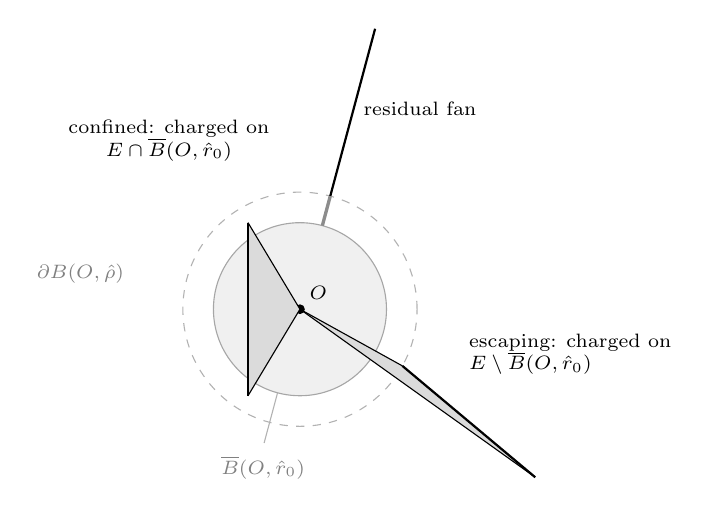
\begin{tikzpicture}[scale=2.2,>={Stealth[length=2mm]}]
  \coordinate (O) at (0,0);
  \fill[black!6] (O) circle (0.4995);
  \draw[gray!70] (O) circle (0.4995);
  \draw[gray!60,dashed] (O) circle (0.676);
  \fill (O) circle (0.8pt) node[above right,font=\scriptsize]{$O$};
  \draw[gray!60] (255:0.4995) -- (255:0.80);
  \node[gray,font=\scriptsize,below] at (255:0.82) {$\overline B(O,\hat r_{0})$};
  \node[gray,font=\scriptsize,left] at (168:0.98) {$\partial B(O,\hat\rho)$};
  \fill[black!14] (O) -- (-0.30,0.50) -- (-0.30,-0.50) -- cycle;
  \draw[thick] (-0.30,0.50) -- (-0.30,-0.50);
  \draw (O) -- (-0.30,0.50); \draw (O) -- (-0.30,-0.50);
  \node[font=\scriptsize,align=center,anchor=south east] at (-0.12,0.80)
    {confined: charged on\\ $E\cap\overline B(O,\hat r_{0})$};
  \fill[black!14] (O) -- (0.591,-0.327) -- (1.358,-0.970) -- cycle;
  \draw[thick] (0.591,-0.327) -- (1.358,-0.970);
  \draw (O) -- (0.591,-0.327); \draw (O) -- (1.358,-0.970);
  \node[font=\scriptsize,align=left,anchor=west] at (0.92,-0.26)
    {escaping: charged on\\ $E\setminus\overline B(O,\hat r_{0})$};
  \draw[thick] (75:0.676) -- (75:1.676);
  \draw[very thick,black!45] (75:0.4995) -- (75:0.676);
  \node[font=\scriptsize,anchor=west] at (75:1.20) {residual fan};
\end{tikzpicture}
\caption{The additive mechanism of Sections~\ref{sec:additive}
and~\ref{sec:annbudget}, not to scale. The plane, not the direction circle, is
split: the closed ball $\overline B(O,\hat r_{0})$ is measurable, so
Carath\'eodory splitting \eqref{eq:annsplit} is exact for the possibly
nonmeasurable set $E$. A confined direction is charged only through the part of
its triangle inside the ball, an escaping direction only through the part
outside it, and a direction surviving every deletion is charged through the
annulus $\hat r_{0}<|x|\le\hat\rho$ swept by its needle's ray. Nothing is
charged twice, so the two ledgers add instead of competing.}
\label{fig:annsplit}
\end{figure}

% ---------------------------------------------------------------------
\section{Assembly of the main theorem}\label{sec:assembly}

\emph{Input:} the three branch bounds of
Sections~\ref{sec:trichotomy}--\ref{sec:caseII}, the four gates of
Section~\ref{sec:anngates}, and the explicit witness of Part~\ref{part:upper}.
\emph{Goal:} Theorem~\ref{thm:A}. \emph{Mechanism:} the trichotomy is
exhaustive, so the smallest of the three baseline branch bounds is a universal
lower bound; the refinement improves that bound by the additive ledger; the
infimum of the class is then squeezed between the refined bound and the area of
one admissible set. \emph{Output:} Theorem~\ref{thm:lower} and
Theorem~\ref{thm:A}.

\begin{theorem}[universal lower bound, baseline route]\label{thm:lower}
Every star-shaped Kakeya set $E\subset\R^{2}$, with no measurability assumption,
satisfies
\[
  \Lout(E)>\frac{100\pi}{5599}.
\]
\end{theorem}

\begin{proof}
Translate the star centre to the origin; this preserves outer measure. If some
chosen triangle has height at least $h_{0}$, Lemma~\ref{lem:high} applies. Otherwise
the height cap \eqref{eq:nohigh} holds and Lemma~\ref{lem:trichotomy} leaves
alternatives (I) and (O), settled by Propositions~\ref{prop:caseI} and
\ref{prop:caseII} respectively. In each case $\Lout(E)>\pi T=100\pi/5599$. The
three branch bounds are collected in Table~\ref{tab:branches}.
\end{proof}

Theorem~\ref{thm:annular} of Section~\ref{sec:anngates} is the stronger
statement, proved by the additive route at the tuple \eqref{eq:annparams}; it
supersedes Theorem~\ref{thm:lower} numerically but not logically, since the two
proofs are independent and the baseline one remains valid. The lower endpoint
of Theorem~\ref{thm:A} is the refined constant.

\begin{table}[t]
\centering
\small
\begin{tabular}{@{}llll@{}}
\toprule
Branch & Normalised form & Strict lower bound for $\Lout(E)$ & Numerical value \\
\midrule
high (H) & $h_{0}/(2\pi)$ & $h_{0}/2$ & $0.0561500$\\
confined (I) & $A_{0}+pX$ & $\pi\bigl(pk\Istar+f_{0}/4\bigr)$ & $0.0561105$\\
escaping (O) & $(1-p)Y\kappa$ & $(1-p)\pi\,c\kappa/4$ & $0.0561116$\\
\midrule
target & $T$ & $\pi T=100\pi/5599$ & $0.0561099$\\
\bottomrule
\end{tabular}
\caption{The three branches of the baseline Theorem~\ref{thm:lower}, in the
normalised form of \eqref{eq:designbounds} and as area bounds. Each branch bound
exceeds the baseline target $T=100/5599$; the decimals are displays of exact
rational comparisons, and the smallest margin is about $6\times10^{-7}$ in
absolute area. The corresponding table for the refinement, at the target
$\hat T=131/6250$, is Table~\ref{tab:anngates}.}
\label{tab:branches}
\end{table}

\begin{proof}[Proof of Theorem~\ref{thm:A}]
Part (i) is Theorem~\ref{thm:annular}. Taking the infimum over all star-shaped
Kakeya sets in (i) gives $\Astar\ge131\pi/6250$ --- non-strictly, as explained in
Remark~\ref{rem:strict}. Part (ii) is Theorem~\ref{thm:upper}, and since
$E_{100001}$ is itself a star-shaped Kakeya set,
\[
  \Astar\le|E_{100001}|<\frac{77\pi}{851}.
\]
Combining the two displays proves Theorem~\ref{thm:A}. Corollary~\ref{cor:historical}
follows from $131/6250>1/98$, indeed $(131/6250)\cdot98=6419/3125$, and from the
last two inequalities in Theorem~\ref{thm:upper}.
\end{proof}

\begin{corollary}\label{cor:turning}
The same two-sided estimate holds for the continuous-turning constant:
\[
  \frac{131\pi}{6250}\ \le\ \Aturn\ <\ \frac{77\pi}{851}.
\]
\end{corollary}

\begin{proof}
Every admissible set is a star-shaped Kakeya set, so Theorem~\ref{thm:annular}
applies to it and the infimum $\Aturn$ inherits the non-strict lower bound; the
upper bound is Theorem~\ref{thm:upper}, which bounds $\Aturn$ directly because
$E_{100001}$ is admissible.
\end{proof}

% =====================================================================
\section{Discussion and open problems}\label{sec:discussion}

\paragraph{The remaining gap.} The ratio between the endpoints of
Theorem~\ref{thm:A} is $(77/851)\cdot(6250/131)=481250/111481=4.3168\ldots$, down
from $5.066\ldots$ for the baseline constant, so the true value of $\Astar$ is
still far from determined. Both endpoints are proved by fixed-parameter
arguments with small margins. Neither of the parameter searches was carried out
to completion, so re-optimisation within the present methods may still improve
the constants; what appears to require new structure is a substantial closure of
the remaining four-fold gap, and we do not know how large the improvement
obtainable by re-optimisation alone is.

\paragraph{Richer profile families for the upper bound.} The set $E_{100001}$ is
a witness, not a candidate extremiser, and we make no claim of optimality for
the profile pair \eqref{eq:aprofile}--\eqref{eq:sprofile}: neither within the
polynomial family \eqref{eq:ansatz}, nor among admissible sets. The room visible in
Section~\ref{sec:finitelift} is only certificate and display slack --- the
outward rounding in \eqref{eq:contbound}, the allowance
\eqref{eq:areaerror}, and the compression of the certified endpoint into
$77/851$ --- and exhausting all of it would move the constant by less than
$10^{-5}$ in normalised area. Reducing the upper endpoint substantially is a
different question: whether the design constraints of
Section~\ref{sec:signrole} admit profiles with a strictly smaller limiting
area, and, more structurally, whether the two-branch envelope of
Proposition~\ref{prop:branches} is forced by those constraints or is an artefact
of the polynomial ansatz. Nothing here proves that a better profile exists. A family whose envelope
has a different active-branch pattern would need a new completeness argument,
which is where the mathematical difficulty lies.

\paragraph{Stronger mechanisms for the lower bound.} The second of the two
directions listed in the previous version of this discussion --- exploiting the
interaction between the confined and the escaping class instead of treating them
as alternatives --- is what
Sections~\ref{sec:additive} and~\ref{sec:annbudget} carry out, and it moved the
lower endpoint by $17.36\%$. The mechanism is now itself limited by two nearly
tied gates, ($\widehat{\mathrm{C}}1$) and ($\widehat{\mathrm{C}}2$) of
Table~\ref{tab:anngates}: the high branch and the raw radial integral. The
exterior gates ($\widehat{\mathrm{C}}3$), ($\widehat{\mathrm{C}}4$) have margins
larger by three orders of magnitude, so the exterior geometry is no longer the
bottleneck, and the sharp one-sided width $W_{\hat\rho}$ of
Lemma~\ref{lem:annwidth}, which is proved but deliberately unexploited
(Remark~\ref{rem:annweak}), would buy nothing at present. What would help is
therefore a better \emph{interior} mechanism: a multiscale coupling between the
radial slices of \eqref{eq:radialint}, which are still estimated independently
at each radius, or a dilation loss $\hat g$ smaller than the pointwise maximum
of three worst-case regimes. We do not claim that re-optimising
\eqref{eq:params} or \eqref{eq:annparams} is exhausted, only that the binding
constraint has moved from the exterior to the interior of the argument.

\paragraph{Does continuous turning matter?} We proved $\Astar\le\Aturn$ and, by
Corollary~\ref{cor:turning}, bounded both constants by the same two numbers.
Whether $\Astar=\Aturn$ --- that is, whether requiring a continuous
endpoint-reversing motion changes the infimum for star-shaped sets --- is open. A
separation would exhibit a star-shaped Kakeya set that cannot be approximated by
turning constructions; an equality would presumably come from a general
procedure turning a pointwise needle family into a continuous motion at
arbitrarily small area cost.

% =====================================================================
\appendix

\section{Exact constants and certificate data}\label{app:constants}

This appendix records the exact data on which the main text relies, and the
shape of the algebraic certificates that produce them. All arithmetic below is
exact: rational, or rational over $\Q(\sqrt2)$, with outward rounding wherever
an enclosure is used.

\subsection{Upper bound}

\paragraph{Sign certificates.} Proposition~\ref{prop:signs} asserts strict signs
for the polynomials $s$, $s''$, $\Hsup$, $\Hsup'$, $\Hsup-s'$ and $J$ of
\eqref{eq:signs}--\eqref{eq:J} on rational subintervals of $[0,1]$. Each is
proved by a centred-Horner expansion with rational endpoints followed by a
Bernstein positivity test: on each subinterval the expanded coefficient vector
has a constant strict sign, which certifies the sign of the polynomial there.
The expansions are re-derived inside the formalisation from the definitions of
$a$ and $s$, so the generated data are inputs, not oracles.

\paragraph{Switch isolation.} Lemma~\ref{lem:switch} eliminates the system
\eqref{eq:switch} to a univariate resultant over $\Q(\sqrt2)$, isolates its
roots by exact rational bisection with Sturm sequences, and recovers the second
coordinate by a subresultant/B\'ezout identity. The certificate consists of five
pairs of rational isolating boxes for $(\tau_{i},\zeta_{i})$, together with the
terminal stationary parameter $\tau_{*}$, and of the sign data proving that the
asserted branch dominates on each of the six intervals. Completeness --- that
there are exactly five solutions --- is part of the certificate, since the
resultant's root count is certified rather than sampled.

\paragraph{Area primitives.} The two antiderivatives of
Section~\ref{sec:envelope} are polynomials in $\Q(\sqrt2)[t]$, namely
$\Ps'=-ss''$ and $\Pe'=J$. The six-piece expression \eqref{eq:sixpiece} is
evaluated by interval-evaluating each of the twelve endpoint terms on its
isolating box and summing with outward rounding, giving
\eqref{eq:contbound}.

\paragraph{Finite-cell constants.} At $n=100001$,
\begin{align*}
  \eta&=\eta_{100001}=\frac{6930}{4049667751},
  \qquad
  2\eta+\eta^{2}=\frac{56128443053760}{16399808893489398001},\\[4pt]
  \frac{|E_{100001}|}{\pi}
  &<\frac{90477812}{10^{9}}+\frac{56128443053760}{16399808893489398001}
  <\frac{77}{851}<\frac{5-2\sqrt2}{24},
\end{align*}
the last inequality by $5-24\cdot\frac{77}{851}=\frac{2407}{851}$ and
$\bigl(\frac{2407}{851}\bigr)^{2}-8=\frac{41}{851^{2}}>0$.

\subsection{Lower bound, baseline route}

\paragraph{Fixed parameters and derived constants.} The tuple \eqref{eq:params}
and
\[
  f_{0}=\frac{5418677}{62500000000},
  \qquad
  k=\frac{12262791}{12265000},
  \qquad
  T=\frac{100}{5599}.
\]
The derived radii \eqref{eq:derived}--\eqref{eq:R1} satisfy the domain
inequalities \eqref{eq:domain}; the enclosures actually used downstream are
$d\in(302738,302739)/10^{7}$ and $R_{1}>185813/10^{5}$, together with rational
one-sided envelopes for the square roots and for $\arcsin(h_{0}/\rho)$.

\paragraph{Radial integral.} The stored rational lower bound of
Proposition~\ref{prop:integral} is
\[
  \Istar=\frac{22793357350571006116275623711763}
              {1064174925446566790615478200000000},
\]
and the certified chain is $\Istar\le C_{\mathrm{cut}}\le I$ as in
\eqref{eq:Istarchain}, where $C_{\mathrm{cut}}$ uses the safe cuts
$L=9/40$ and $U=2353/10000$ and a truncated odd-power logarithm series with an
explicit geometric tail.

\paragraph{Branch margins.} The confined branch margin is the exact rational
number
\[
  p\,k\,\Istar+\frac{f_{0}}{4}-T
  =\frac{139158989937085958631189100903645702101397}
         {664352167944649011863150962260700000000000000000}
  =2.0946\ldots\times10^{-7},
\]
and the escaping branch comparison is $T/(1-p)<c\kappa/4$, proved from
$\kappa>99999/100000$ and the certified enclosure of $\arcsin(h_{0}/\rho)$. The
high branch uses a stored rational upper bound for $\pi$ to compare $h_{0}/2$ with
$\pi T$.

\paragraph{Negative controls.} Two deliberately weakened variants are retained
in the formal development as fail-closed checks: replacing $\Istar$ by a weaker
logarithmic tail makes the confined branch fall below $T$, and shifting $p$
makes the two mass-dependent branches fail to hold simultaneously. On the upper
side, strengthening the continuum target or lowering the cell count to
$n=80001$ makes the corresponding comparison fail.

\subsection{Additive refinement}\label{app:annconstants}

\paragraph{Fixed parameters.} The tuple \eqref{eq:annparams},
\[
  \hat h_{0}=\frac{13177}{100000},
  \qquad
  \hat r_{\lambda}=\frac{10227}{50000},
  \qquad
  \hat r_{0}=\frac{999}{2000},
  \qquad
  \hat\lambda=\frac{29496}{36773},
  \qquad
  \hat T=\frac{131}{6250},
\]
with $\epsdel=10^{-10}$ and $m=1-\epsdel$. The interpolation identity
$\hat\lambda\hat h_{0}+(1-\hat\lambda)\hat r_{0}=\hat r_{\lambda}$ of
\eqref{eq:anndomain} is exact in $\Q$.

\paragraph{Derived radii.} All square roots are enclosed by rationals with
outward rounding, and only the displayed one-sided endpoints are used
downstream:
\begin{align*}
  \sqrt{\hat Q}&\in\bigl(0.39100998140,\ 0.39100998141\bigr), &
  \hat d&\in\bigl(0.03943852316,\ 0.03943852317\bigr),\\
  \sqrt{\hat r_{\lambda}^{2}-\hat d^{2}}
    &\in\bigl(0.20070180490,\ 0.20070180491\bigr), &
  \sqrt{1+4\hat d^{2}}&\in\bigl(1.00310597069,\ 1.00310597070\bigr),\\
  \hat R_{1}&\in\bigl(1.675763481,\ 1.675763482\bigr), &
  \hat\rho&\in\bigl(0.675763481,\ 0.675763482\bigr).
\end{align*}
Each enclosure is proved by squaring, so no transcendental function is
involved. The domain conditions \eqref{eq:anndomain} follow from them by exact
rational comparison; in particular $\hat\rho>\hat r_{0}$ needs only
$0.675763481>0.4995$, and $\hat h_{0}<m\hat\rho$ needs only
$0.13177<(1-10^{-10})\cdot0.675763481$.

\paragraph{The arcsine of the weight.} Gate ($\widehat{\mathrm{C}}3$) needs an
upper bound for $\hat H(\hat h_{0})=\arcsin\bigl(\hat h_{0}/(m\hat\rho)\bigr)$,
because that quantity sits in a denominator. From the enclosure of $\hat\rho$,
\[
  \frac{\hat h_{0}}{m\hat\rho}<\frac{1949945}{10^{7}},
  \qquad
  \arcsin\frac{\hat h_{0}}{m\hat\rho}<\frac{196255}{10^{6}},
\]
the second from the first by the elementary lower bound
$\sin x\ge x-x^{3}/6$ on $[0,1]$, which is enough because both sides are then
compared by exact rational arithmetic. Consequently
\[
  \hat C_{\mathrm{ext}}
  >\frac{\hat h_{0}}{2\cdot196255/10^{6}}-\frac{m\,\hat r_{0}^{2}}{2}
  >0.2109,
  \qquad
  \frac{\hat C_{\mathrm{ext}}}{4}>0.052740>\hat T .
\]

\paragraph{Radial integral.} The refinement does \emph{not} reuse the
three-piece cut of Proposition~\ref{prop:integral}: by
Remark~\ref{rem:annfrozen} the frozen entry of $\hat g$ is inactive at this
tuple, and the maximum switches exactly once, at $0.2352988\ldots$. The
certificate therefore uses two rational cuts straddling that switch,
\[
  q_{L}=\frac{23529}{100000},
  \qquad
  q_{R}=\frac{2353}{10000},
\]
discards the tiny middle interval $[q_{L},q_{R}]$ --- discarding is legitimate
because the integrand is nonnegative --- and bounds the two retained segments
separately:
\[
  \int_{\hat h_{0}}^{q_{L}}\frac{r}{\hat g(r)}\,dr\ \ge\ \frac{732633}{10^{8}},
  \qquad
  \int_{q_{R}}^{\hat r_{0}}\frac{r}{\hat g(r)}\,dr\ \ge\ \frac{136446}{10^{7}},
  \qquad
  \hat I\ \ge\ \hat I_{*}=\frac{2097}{100000}.
\]
On the left segment $\hat g$ is the large-angle entry
$\pi/(\pi/2-\arctan 2r)$, so the primitive involves $\arctan$; it is bounded
below by a six-term odd-power partial sum, with the reflection identity
$\arctan x=\pi/4-\arctan\frac{1-x}{1+x}$ used at the right end to keep every
argument inside the region where the truncation is a lower bound, and $\pi$ is
enclosed by the twenty-digit rationals
$3.14159265358979323846<\pi<3.14159265358979323847$. On the right segment
$\hat g$ is the interior entry $(1+2r)/(1-2r)$, whose primitive is
$-r^{2}/2+r-\tfrac12\log(1+2r)$; the logarithmic increment is bounded above by
the odd-power series in $z=x/(x+2)$ with $x=(1+2\hat r_{0})/(1+2q_{R})-1$, so
that $z=1321/8674$, truncated after three terms with the tail
\[
  \sum_{k\ge3}\frac{2z^{2k+1}}{2k+1}\ \le\ \frac{2z^{7}}{7(1-z^{2})} .
\]
The factor $1/7$ in this tail is load bearing: with the cruder tail
$2z^{7}/(1-z^{2})$ the same two segments fall strictly \emph{below}
$\hat I_{*}$, and that weakened variant is retained in the formal development as
a negative control.

\paragraph{Gate margins.} With $\hat T=131/6250=0.02096$,
\[
  \frac{\hat h_{0}}{2\pi}>0.020971846,
  \qquad
  \hat I\ge\hat I_{*}=0.02097,
  \qquad
  \frac{\hat C_{\mathrm{ext}}}{4}>0.052740,
  \qquad
  \hat C_{\mathrm{fan}}>0.103578,
\]
the last from $\hat\rho>0.675763481$ and $\hat r_{0}=0.4995$. The two binding
margins are $1.18\cdot10^{-5}$ and $1.0\cdot10^{-5}$; the two exterior margins
exceed $3\cdot10^{-2}$.

\paragraph{Negative controls.} Four deliberately weakened variants are retained
in the formal development as fail-closed checks: the crude logarithmic tail just
described; the target raised to $2098/100000$, which the two segments fail to
clear; the assertion that the frozen entry of $\hat g$ is strictly dominated
already at $r=\hat h_{0}$, which pins Remark~\ref{rem:annfrozen}; and the
statement that the two cuts $q_{L},q_{R}$ really straddle the single switch, so
that neither retained segment may be extended across the gap.

\paragraph{Independent numerical evidence.} An interval certificate in
outward-rounded Arb arithmetic at $256$ bits, with the integral bounded below on
an exact rational partition of $[\hat h_{0},\hat r_{0}]$ into $2^{16}$ cells,
reports
\[
  \hat I\ \ge\ 0.020970691554\ldots,
  \qquad
  \hat C_{\mathrm{ext}}\ \ge\ 0.210966886763\ldots,
  \qquad
  \hat C_{\mathrm{fan}}\ \ge\ 0.103578016282\ldots,
\]
together with all domain conditions and four mutation controls. This is
evidence in the sense of Section~\ref{sec:evidence}: it is consumed neither by
the Lean proof nor by the exact-rational proof of this manuscript, both of which
establish the gates independently from the rational data displayed above. Its
one genuine consumer is the conditional paper-level proof note that accompanies
the development, whose Hypotheses B and C it discharges; that note is prose and
is not machine checked.

% ---------------------------------------------------------------------
\section{Formalisation architecture and trusted computing base}
\label{app:formalization}

\subsection{Two developments, one pinned toolchain}

The mathematics above is accompanied by two Lean~4 developments, one for each
half of Theorem~\ref{thm:A}. Both pin the same Lean toolchain and the same
Mathlib revision:
\begin{quote}\small\raggedright
\lean{leanprover/lean4:v4.30.0-rc2}\\
\lean{5450b53e5ddc75d46418fabb605edbf36bd0beb6}
\end{quote}
Under the namespace
subdirectories, the lower development has $54$ modules and the upper development
has $40$ modules; each project also has one top-level aggregation file. Counting
lines with \lean{wc -l}, excluding the build directory and the API probes, the
lower namespace modules total $25\,255$ lines and its $104$-line aggregation
root brings the development to $55$ files and $25\,359$ lines; the upper
development contains $12\,100$ lines on the same convention. The
lower development grew from $35$ to $54$ modules when the additive refinement of
Sections~\ref{sec:additive} and~\ref{sec:annbudget} was formalised; the modules
carrying the baseline route were not modified. Neither development contains any
occurrence of \lean{sorry}, \lean{admit}, a custom \lean{axiom} declaration or
\lean{native\_decide} in the lower half; a reproducible scan is given in
Appendix~\ref{app:repro}.

Several formal identifiers below contain the internal name \lean{RationalSeven}.
This is a project-internal label for the explicit polynomial profile
construction of Section~\ref{sec:construction}; it carries no mathematical
meaning and is retained here only so that the names in the tables match the
source files verbatim.

\subsection{Statement map}

Tables~\ref{tab:lowerlean}--\ref{tab:upperlean} connect the statements of this
paper to the formal ones: the baseline lower route, the additive refinement in
two halves, and the upper construction, in that order. Each row names
the strongest declaration that owns the paper statement; auxiliary lemmas used
only inside a proof are not listed.

The lower endpoint of Theorem~\ref{thm:A} is Theorem~\ref{thm:annular}, and its
formal owner is the module \lean{AnnularAssembly.lean}. That module states the
bound twice: once through the defined target, and once with the constant in
normal form.
\begin{quote}\small\raggedright
\lean{theorem universal\_annular\_lower\_bound :}\\
\hspace*{1em}\lean{$\forall$ (E : Set Plane), StarShapedKakeya E $\to$}\\
\hspace*{1em}\lean{ENNReal.ofReal (Real.pi * annTarget)}\\
\hspace*{3em}\lean{< volume.toOuterMeasure E}\\[3pt]
\lean{theorem universal\_annular\_lower\_bound\_normalForm}\\
\hspace*{1em}\lean{(E : Set Plane) (K : StarShapedKakeya E) :}\\
\hspace*{1em}\lean{ENNReal.ofReal (131 * Real.pi / 6250)}\\
\hspace*{3em}\lean{< volume.toOuterMeasure E}
\end{quote}
Here \lean{annTarget = 131 / 6250} is defined in \lean{AnnularKernel.lean}. The
final theorem of the baseline route, namely
\lean{universal\_strong\_lower\_bound}, is untouched by this development and
still compiles; the two final lower theorems are import-disjoint above their
shared base, and the transitive import closure of the new assembly module
contains none of the baseline frozen-constant modules.

\begin{table}[t]
\centering
\footnotesize
\begin{tabular}{@{}>{\raggedright\arraybackslash}p{0.35\textwidth}>{\raggedright\arraybackslash}p{0.57\textwidth}@{}}
\toprule
Paper statement & Lean statement / module \\
\midrule
Definition~\ref{def:ssk}, triangle family
  & \lean{StarShapedKakeya}, \lean{needleFamily}, \lean{triangleHull\_subset}
    (\lean{StarKakeyaSet.lean})\\
Lemma~\ref{lem:triangle}
  & \lean{TriangleAreaBridge}, \lean{triangleAreaBridge}
    (\lean{TriangleArea.lean})\\
Parameters \eqref{eq:params}, domain \eqref{eq:domain}
  & \lean{strongParameterDomain} (\lean{StrongerKernel.lean})\\
Lemma~\ref{lem:trichotomy}
  & \lean{direction\_radius\_trichotomy} (\lean{Trichotomy.lean})\\
Lemma~\ref{lem:high}
  & \lean{high\_branch\_outerMeasure},
    \lean{strong\_target\_lt\_high\_threshold}\\
First arcs, $\Gamma_{\alpha}$, $J\Gamma_{\alpha}$
  & \lean{supportTraceFirstArcData} (\lean{UniversalFirstArc.lean}),
    \lean{universalArcData} (\lean{UniversalEndpointClosure.lean})\\
Proposition~\ref{prop:endpoint}
  & \lean{universal\_hybrid\_containment}
    (\lean{UniversalEndpointClosure.lean})\\
Lemma~\ref{lem:localcontact}
  & \lean{figure5LocalContactCertificate\_of\_actualSelected},
    \lean{figure5\_local\_contact\_pointwise}
    (\lean{Figure5LocalContact.lean})\\
Remark~\ref{rem:counterexample}
  & \lean{exterior\_arcsin\_dispatch\_counterexample}
    (audit-only \lean{NegativeControls.lean})\\
Lemma~\ref{lem:dilation}
  & \lean{volume\_iUnion\_quotientHybridCenteredDilate\_le}
    (\lean{QuotientCircle.lean})\\
Lemma~\ref{lem:polar}
  & \lean{outerMeasure\_ge\_lintegral\_of\_angleOuter\_ge}
    (\lean{PolarOuterMeasure.lean}),
    \lean{volume\_projectedPolar\_le\_cutOuter}
    (\lean{PolarProjectiveOuter.lean})\\
Estimate \eqref{eq:radialint}
  & \lean{angleOuter\_ge\_of\_firstArcPointwiseAggregate},
    \lean{outerMeasure\_inner\_ge\_caseI\_lintegral\_of\_raw}\\
Proposition~\ref{prop:integral}
  & \lean{strong\_integral\_certificate\_ge}, \lean{strongILower\_le\_integral}
    (\lean{CaseIStrongIntegral.lean})\\
Proposition~\ref{prop:li25}
  & \lean{strongLiLemma25} (\lean{StrongLiLemma25.lean})\\
Proposition~\ref{prop:caseI}
  & \lean{strong\_caseI\_margin\_exact}, \lean{strong\_caseI\_strict}\\
Lemma~\ref{lem:outside}
  & \lean{outsideBall\_sub\_one\_of\_not\_triangleHull\_subset\_closedBall}\\
Lemma~\ref{lem:shadow}
  & \lean{UnitNeedle.triangleRayControlled\_of\_outside},
    \lean{pairwise\_disjoint\_triangleInterior\_of\_outside}
    (\lean{CaseIIGeometry.lean}); the separation hypothesis is supplied by
    \lean{future\_triangle\_shadow\_sum\_lt\_distance}
    (\lean{CaseIISelection.lean})\\
Proposition~\ref{prop:budget}
  & \lean{fixedSelectionOutcome},
    \lean{directionAngleOuter\_fixedDeletionBall\_le}
    (\lean{CaseIISelection.lean}), \lean{greedyResidual}
    (\lean{GreedyResidual.lean})\\
Proposition~\ref{prop:caseII}
  & \lean{caseII\_fixed\_greedy\_lower\_bound},
    \lean{strong\_caseII\_fixed\_coefficient\_strict},
    \lean{strongCaseII\_radius\_branch}\\
Theorem~\ref{thm:lower}
  & \lean{universal\_strong\_lower\_bound} (\lean{UniversalAssembly.lean})\\
\bottomrule
\end{tabular}
\caption{Lower bound, baseline route: paper-to-Lean map; this development is
unchanged by the additive refinement mapped in
Tables~\ref{tab:annlean} and~\ref{tab:annlean2}. The
final proposition is \lean{$\forall$ E, StarShapedKakeya E $\to$ ofReal ($\pi$ * 100 / 5599) <
volume.toOuterMeasure E}.}
\label{tab:lowerlean}
\end{table}

\begin{table}[t]
\centering
\footnotesize
\begin{tabular}{@{}>{\raggedright\arraybackslash}p{0.35\textwidth}>{\raggedright\arraybackslash}p{0.57\textwidth}@{}}
\toprule
Paper statement & Lean statement / module \\
\midrule
Parameters \eqref{eq:annparams}, derived radii
  \eqref{eq:annderived}--\eqref{eq:annR1}, domain \eqref{eq:anndomain}
  & \lean{annA}, \lean{annRLambda}, \lean{annR$_{0}$}, \lean{annEps},
    \lean{annLambda}, \lean{ann\_lambda\_affine\_identity},
    \lean{ann\_r$_{1}$\_lower}, \lean{ann\_rho\_lower},
    \lean{annA\_lt\_annM\_mul\_annRho} (\lean{AnnularKernel.lean})\\
Carath\'eodory split \eqref{eq:annsplit}, Lemma~\ref{lem:anncara}
  & \lean{outerMeasure\_split\_closedBall},
    \lean{outerMeasure\_ge\_add\_of\_inter\_of\_diff} (\lean{BallSplit.lean})\\
Lemma~\ref{lem:annsuper}, Corollary~\ref{cor:annledger}
  & \lean{tsum\_outerMeasure\_inter\_le} (\lean{BallSplit.lean}),
    \lean{tsum\_volume\_restrictedTriangle\_le\_outerMeasure}
    (\lean{AnnularGreedyInfinite.lean})\\
Lemmas~\ref{lem:annonesided} and~\ref{lem:annwidth}, weak form
  & \lean{UnitNeedle.exists\_arcSector\_of\_outside}
    (\lean{AnnularGeometry.lean})\\
Proposition~\ref{prop:annexterior}
  & \lean{UnitNeedle.volume\_triangleHull\_diff\_closedBall\_ge},
    \lean{UnitNeedle.volume\_triangleInterior\_diff\_closedBall}\\
Lemmas~\ref{lem:annchord} and~\ref{lem:annarcsin}
  & \lean{sin\_chord\_le}, \lean{arcsin\_mul\_sin\_le}\\
Proposition~\ref{prop:annpayment}
  & \lean{annularCExt}, \lean{UnitNeedle.annular\_payment},
    \lean{UnitNeedle.annular\_payment\_triangleInterior}\\
Lemmas~\ref{lem:annshadowcone} and~\ref{lem:annconedisjoint}
  & \lean{UnitNeedle.triangleRayControlled\_of\_outside},
    \lean{pairwise\_disjoint\_triangleInterior\_of\_outside}
    (\lean{CaseIIGeometry.lean}); transferred to the exterior parts by
    \lean{FiniteFixedSelection.pairwise\_disjoint\_restrictedTriangle}
    (\lean{AnnularGreedy.lean}) in the finite case and by
    \lean{FixedDeletionGreedyData.pairwise\_disjoint\_restrictedTriangle}
    (\lean{AnnularGreedyInfinite.lean}) in the countable case\\
\bottomrule
\end{tabular}
\caption{Additive refinement, first half: the parameter tuple, the additive
outer-measure ledger and the one-sided annular geometry. Each row names the
strongest declaration that owns the paper statement.}
\label{tab:annlean}
\end{table}

\begin{table}[t]
\centering
\footnotesize
\begin{tabular}{@{}>{\raggedright\arraybackslash}p{0.35\textwidth}>{\raggedright\arraybackslash}p{0.57\textwidth}@{}}
\toprule
Paper statement & Lean statement / module \\
\midrule
Selection \eqref{eq:annselect}, Lemma~\ref{lem:annbudgetineq} (B1)--(B3)
  & \lean{future\_triangle\_shadow\_sum\_lt\_distance},
    \lean{directionAngleOuter\_fixedDeletionBall\_le}
    (\lean{CaseIISelection.lean}),
    \lean{cost\_le\_tsum\_volume\_restrictedTriangle},
    \lean{quarter\_cost\_le\_outerMeasure\_infinite}\\
Lemma~\ref{lem:annbudgetineq} (B4)
  & \lean{selected\_height\_tendsto\_zero\_of\_summable},
    \lean{residual\_height\_zero\_of\_summable\_paperWeight}\\
Lemmas~\ref{lem:anncut} and~\ref{lem:annfan}
  & \lean{euclideanPolarAnnulus\_outerMeasure\_ge},
    \lean{residualFan\_annulus\_outerMeasure\_lower}
    (\lean{AnnularGreedy.lean})\\
Ledger \eqref{eq:annledgerA}, case $B=\infty$
  & \lean{outerMeasure\_diff\_eq\_top\_of\_cost\_eq\_top}
    (\lean{AnnularGreedyInfinite.lean})\\
Ledger \eqref{eq:annledgerB}, Proposition~\ref{prop:annbudget}
  & \lean{annular\_exterior\_lower\_bound\_of\_summable},
    \lean{annular\_exterior\_greedy\_lower\_bound},
    \lean{annular\_exterior\_A\_out\_greedy\_lower\_bound}
    (\lean{AnnularGreedyInfinite.lean})\\
Parametric reuse of Section~\ref{sec:caseI}
  & \lean{Figure5EndpointDomain},
    \lean{Figure5EndpointAnalyticPackage}
    (\lean{Figure5EndpointDomain.lean}); instances
    \lean{annFigure5Domain}, \lean{annFigure5AnalyticPackage}
    (\lean{AnnularEndpoint.lean})\\
Proposition~\ref{prop:annsection}
  & \lean{angleOuter\_ge\_of\_firstArcPointwiseAggregate},
    \lean{annular\_aggregateMass\_of\_directionOuterMass}
    (\lean{CaseIRadialCore.lean}),
    \lean{universal\_confined\_lower\_bound\_of\_trace\_containment}
    (\lean{AnnularCaseI.lean})\\
Proposition~\ref{prop:annconfined}
  & \lean{confined\_lower\_bound\_of\_endpointDomain}
    (\lean{EndpointConfinedExit.lean}),
    \lean{annular\_confined\_lower\_bound} (\lean{AnnularEndpoint.lean})\\
Proposition~\ref{prop:anngates}
  & \lean{ann\_gate\_C1}, \lean{ann\_gate\_C3}, \lean{ann\_gate\_C4},
    \lean{ann\_gate\_min\_exterior} (\lean{AnnularAnalytic.lean}),
    \lean{annILower\_le\_lintegral}, \lean{annTarget\_lt\_annILower}
    (\lean{AnnularCaseIIntegral.lean}),
    \lean{ann\_certificate\_sum\_ge\_target} and the negative controls
    (\lean{AnnularIntegralControls.lean})\\
Theorem~\ref{thm:annular}
  & \lean{annular\_joint\_ledger}, \lean{annular\_lower\_bound},
    \lean{universal\_annular\_lower\_bound},
    \lean{universal\_annular\_lower\_bound\_normalForm}
    (\lean{AnnularAssembly.lean})\\
\bottomrule
\end{tabular}
\caption{Additive refinement, second half: greedy budget, confined
contribution, numerical gates, final assembly. The final source owner is the
assembly module quoted before the tables.}
\label{tab:annlean2}
\end{table}

\begin{table}[t]
\centering
\footnotesize
\begin{tabular}{@{}>{\raggedright\arraybackslash}p{0.35\textwidth}>{\raggedright\arraybackslash}p{0.57\textwidth}@{}}
\toprule
Paper statement & Lean statement / module \\
\midrule
Definitions~\ref{def:turning}, \ref{def:admissible}
  & \lean{TurningNeedle}, \lean{AdmissibleWitness}, \lean{Admissible}
    (\lean{Definitions.lean})\\
Profiles \eqref{eq:Apoly}--\eqref{eq:sprofile}, symmetries \eqref{eq:reflect}
  & \lean{normalProfile\_reflect}, \lean{tangentProfile\_reflect}
    (\lean{RationalSevenProfiles.lean})\\
Construction \eqref{eq:c0}--\eqref{eq:Edef}
  & \lean{RationalSeven.E} (\lean{RationalSeven.lean})\\
$n=100001$ instance of Proposition~\ref{prop:admissible}
  & \lean{localCenter\_join}, \lean{cellCenter\_join},
    \lean{cellDirection\_join}, \lean{motion\_oriented},
    \lean{endpoints\_reversal}, \lean{star\_shaped}, \lean{isCompact\_E},
    \lean{admissible}\\
Proposition~\ref{prop:signs}
  & \lean{RationalSevenSigns.lean}\\
Proposition~\ref{prop:branches}
  & \lean{RationalSevenEnvelope.lean}, the global contact/classification modules,
    and \lean{ContinuumDominance.lean} (six dominance-interval theorems)\\
Lemma~\ref{lem:switch}
  & \lean{switch\_system\_complete},
    \lean{SwitchCertificatePhase1/2/3} modules\\
Identity \eqref{eq:sixpiece}
  & \lean{FinalAreaAssembly.six\_piece\_integrals\_eq\_expression}\\
Proposition~\ref{prop:area}
  & \lean{AreaPrimitiveCertificate.sixPieceExpression\_lt}
    (\lean{AreaPrimitiveCertificate.lean}),
    \lean{FinalAreaTheorem.integral\_continuumRadiusReal\_sq\_lt}
    (\lean{FinalAreaTheorem.lean})\\
Proposition~\ref{prop:lift}, constants
  \eqref{eq:finitebranch}--\eqref{eq:areaerror}
  & \lean{RationalSevenFundamentalInterior/Boundary.lean},
    \lean{RationalSevenGlobalPointwise/GlobalArea.lean},
    \lean{RationalSevenPolarFoldBridge.lean},
    \lean{RationalSevenAcuteFold.lean},
    \lean{RationalSevenFiniteSineFactor.lean},
    \lean{RationalSevenNewlyFeasibleEndpoint.lean},
    \lean{RationalSevenFiniteLiftArithmetic.lean}, and
    \lean{RationalSevenAreaErrorIntegration.lean}\\
Theorem~\ref{thm:upper}
  & \lean{rationalSeven\_volume\_lt\_simpleArea},
    \lean{simpleArea\_lt\_cunninghamSchoenberg},
    \lean{rationalSeven\_strictly\_improves\_cunninghamSchoenberg}
    (\lean{FinalAreaTheorem.lean})\\
\bottomrule
\end{tabular}
\caption{Upper bound: paper-to-Lean map. The final theorem has the form
\lean{Admissible E $\wedge$ area E < ofReal cunninghamSchoenbergArea}, with
\lean{E} the literal set \eqref{eq:Edef} at $n=100001$.}
\label{tab:upperlean}
\end{table}

\subsection{Definition alignment}

Table~\ref{tab:alignment} records how the paper's notions correspond to the two
formal vocabularies, since the developments were written independently.

\begin{table}[t]
\centering
\footnotesize
\begin{tabular}{@{}>{\raggedright\arraybackslash}p{0.14\textwidth}
                  >{\raggedright\arraybackslash}p{0.22\textwidth}
                  >{\raggedright\arraybackslash}p{0.20\textwidth}
                  >{\raggedright\arraybackslash}p{0.36\textwidth}@{}}
\toprule
Paper notion & Lower development & Upper development & Alignment note\\
\midrule
plane & \lean{Plane} & \lean{Plane} & both \lean{EuclideanSpace $\R$ (Fin 2)};
  coordinate change is measure preserving\\
star-shaped & \lean{StarShapedKakeya.star} & \lean{StarShapedAt}
  & same notion\\
Kakeya condition & one needle per direction & continuous half-turn
  & upper condition includes additional continuous-turning data\\
size & \lean{volume.toOuterMeasure E} & \lean{volume E}
  & agree because the explicit set is compact\\
directions & \lean{AddCircle $\pi$} & oriented $[0,\pi]$ with reversal
  & both realise the projective circle \eqref{eq:projcircle}; the upper
    development keeps an oriented parameter and quotients by the reversal\\
\bottomrule
\end{tabular}
\caption{Definition alignment between the paper and the two developments.}
\label{tab:alignment}
\end{table}

\subsection{Build evidence and axiom footprint}

On 2 August 2026, in the working tree from which this paper was prepared, the
production and audit builds completed successfully. Build logs are not part of
this document, so we record only the commands and the outcome:
\begin{center}
\small
\begin{tabular}{@{}ll@{}}
\toprule
Command & Result \\
\midrule
\lean{lake build +StarKakeyaLower} & \lean{Build completed successfully}\\
\lean{lake build StarKakeyaLowerAudit} & \lean{Build completed successfully}\\
\lean{lake build +StarKakeya} & \lean{Build completed successfully}\\
\lean{lake build +StarKakeya.Audit} & \lean{Build completed successfully}\\
\bottomrule
\end{tabular}
\end{center}
The audit modules print axiom footprints. The lower audit target emits $477$
receipts, and the set of distinct axiom lists over all of them has exactly one
element; in particular, for the two final lower theorems,
\begin{center}
\lean{'universal\_strong\_lower\_bound' depends on axioms:
  [propext, Classical.choice, Quot.sound]},\\
\lean{'universal\_annular\_lower\_bound' depends on axioms:
  [propext, Classical.choice, Quot.sound]},
\end{center}
i.e.\ only the three standard Mathlib axioms. For the upper theorem,
\lean{rationalSeven\_strictly\_improves\_cunninghamSchoenberg} depends on those
three axioms \emph{and} on $75$ additional reflection axioms generated by scoped
\lean{native\_decide} calls, distributed over the switch-certificate, dominance
and area-primitive modules. This difference is material and we do not paper over
it. No reflection or compiler axiom --- that is, none of \lean{sorryAx},
\lean{Lean.ofReduceBool}, \lean{Lean.ofReduceNat} or
\lean{Lean.trustCompiler} --- occurs anywhere in the lower audit output.

\subsection{Trusted computing base}

We distinguish seven layers.
\begin{enumerate}
  \item The Lean kernel and elaborator.
  \item The pinned toolchain and Mathlib revision listed above.
  \item The conventional Mathlib axioms \lean{propext}, \lean{Classical.choice},
    \lean{Quot.sound}. These suffice for both lower theorems, the baseline one
    and the refinement.
  \item Generated certificate data (switch boxes, primitive enclosures,
    dominance data). These are checked-in files of exact rational data; they are
    inputs to Lean proofs, not oracles.
  \item The $63$ scoped \lean{native\_decide} invocations in the upper
    development, which generate the $75$ reflection axioms noted above. For
    these Boolean reflections the practical trust base includes the Lean
    compiler and native runtime in addition to the kernel. The Mathlib style
    linter warns about exactly this, correctly; the warning is not an error, and
    it does not make those checks purely kernel-reduced.
  \item Python certificate generators (\lean{numpy}, \lean{python-flint},
    \lean{sympy}). They produce candidate data using exact rational and
    $\Q(\sqrt2)$ arithmetic, Sturm/root isolation and outward rational interval
    arithmetic. Their byte-exact \lean{--check} modes and their mutation tests are
    documented in Appendix~\ref{app:repro}. Every mathematical assertion the
    theorems depend on is rechecked inside Lean: formal derivatives, profile
    expansions, centred-Horner enclosures, cover completeness, subresultant
    recovery, B\'ezout identities, switch-system completeness, dominance, and the
    final rational arithmetic.
  \item External arbitrary-precision computations used for exploration and
    secondary cross-checks. These are never promoted into a proof.
\end{enumerate}

\subsection{Evidence boundary}\label{sec:evidence}

We state plainly what the present evidence does and does not establish. The
mathematical content of Theorem~\ref{thm:A} is machine-checked in the two senses
just distinguished: the lower inequality is a conventional Lean proof over
Mathlib with the three standard axioms --- twice over, by the baseline route and
by the additive refinement, the latter being the one that proves the displayed
constant --- and the upper inequality is a Lean proof that additionally reflects
a family of large decidable algebraic checks through native evaluation. Successful builds and clean axiom prints are evidence about
the formal artefacts only. They are not peer review; they do not certify that
Definitions~\ref{def:ssk} and~\ref{def:admissible} are the ones a reader has in
mind (which is why both are spelled out in full, and why
Table~\ref{tab:alignment} exists); and they say nothing about optimality or
priority. In particular, the parameters \eqref{eq:params} and
\eqref{eq:annparams} are fixed data, no derivation identifying either tuple as
canonical or optimal is offered (Remarks~\ref{rem:params}
and~\ref{rem:annprov}), and a search over the full legal domains
\eqref{eq:domain} and \eqref{eq:anndomain} was not completed; the numerical
scout and the interval certificate that accompany the refinement are evidence
about explicit real numbers, consumed neither by the Lean proof nor by the
exact-rational proof of this manuscript, and their role as the discharge of
Hypotheses B and C of the conditional paper-level proof note is a prose
dependency, not a kernel-checked one; likewise the profile pair
\eqref{eq:aprofile}--\eqref{eq:sprofile} and the cell count $n=100001$ are one
certified choice among many, with no minimality claimed.

% ---------------------------------------------------------------------
\clearpage
\section{Reproduction}\label{app:repro}

The canonical one-command reproduction is
\begin{quote}\small\ttfamily
bash scripts/reproduce-core.sh
\end{quote}
This script creates a local environment with \lean{uv}, installs the pinned
\lean{requirements-lock.txt}, runs the symbolic and interval verifiers, checks
generated certificate bytes and mutation tests, and invokes the Lean targets.
For manual execution, first set
\begin{quote}\small\ttfamily\raggedright
export PKG="\$PWD/materials/STAR-SHAPED-KAKEYA-UPPER-LOWER-COMBINED-2026-07-31"\\
export PYTHON="\$PWD/.venv/bin/python"
\end{quote}
after the reproduction script has created \lean{.venv}. Paths below are relative
to the project root. As in Appendix~\ref{app:formalization}, file and script
names such as \lean{RationalSeven} and \lean{pi56} are internal identifiers with
no mathematical content; they are reproduced verbatim so that the commands can
be run as written.

\subsection*{Environment}

\begin{quote}\small\ttfamily\raggedright
Lean toolchain (both developments): leanprover/lean4:v4.30.0-rc2\\
Mathlib revision (both developments):\\
\hspace*{1em}5450b53e5ddc75d46418fabb605edbf36bd0beb6\\
Pinned Python packages: numpy 2.5.1, python-flint 0.9.0,\\
\hspace*{1em}scipy 1.16.2, sympy 1.14.0, mpmath 1.3.0
\end{quote}

On hosts whose soft file-descriptor limit is $1024$, Mathlib cache extraction
fails; the reproduction script raises it when possible, or it may be raised
manually with \verb|ulimit -n 65535|.

\subsection*{Level 1: archive integrity}

\begin{quote}\small\ttfamily
\$PYTHON \$PKG/tools/verify\_combined\_archive.py --self-contained archive/*.zip
\end{quote}
This checks the manifest, the path set, SHA-256 digests and ZIP CRCs.

\subsection*{Level 2: exact and interval certificate generators}

Lower bound, baseline route:
\begin{quote}\small\ttfamily
cd \$PKG/lower-bound/03-computation\\
\$PYTHON verify\_pi56\_noniterative\_kernel.py\\
\$PYTHON verify\_pi56\_parametric\_caseii\_kernel.py\\
\$PYTHON verify\_pi56\_optimization\_reduction.py\\
\$PYTHON verify\_pi56\_stronger\_candidate.py\\
\$PYTHON interval\_pi56\_raw\_family.py
\end{quote}

Lower bound, additive refinement (paths relative to the project root):
\begin{quote}\small\ttfamily
\$PYTHON spikes/001-joint-inner-outer/certify.py\\
\$PYTHON spikes/001-joint-inner-outer/test\_annular\_geometry.py
\end{quote}
The first is the outward-rounded Arb interval certificate of
Appendix~\ref{app:annconstants}: it rechecks the domain conditions
\eqref{eq:anndomain} and the four gates \eqref{eq:anngates} for the frozen tuple
\eqref{eq:annparams}, runs four mutation controls and a static exactness guard
on its fixed path, and writes its certificate next to its own source file; the
one-command reproduction therefore executes it from a temporary copy and then
compares the freshly produced certificate with the tracked one field by field,
allowing only the wall-clock field to differ, so that the tracked file is never
written. The second is a falsification test for the geometry of
Section~\ref{sec:anngeom}: it scans for violations of
Lemma~\ref{lem:annonesided}, checks the sharp width \eqref{eq:annWrho} and the
sector identity behind Proposition~\ref{prop:annexterior} against direct
computation, and includes a power control which does find counterexamples to a
deliberately overstated variant. Neither script is an input to the Lean proof or
to the exact-rational proof of this manuscript, and neither proves anything
about star-shaped Kakeya sets; their one consumer is the conditional
paper-level proof note, whose Hypotheses B and C the certificate discharges in
prose. See Section~\ref{sec:evidence}.

Upper bound:
\begin{quote}\small\ttfamily
cd \$PKG/upper-bound/02-computation\\
\$PYTHON verify\_rational\_seven\_direction.py\\
\$PYTHON verify\_rational\_seven\_continuum\_area.py\\
\$PYTHON verify\_finite\_n\_lift\_bound.py\\
\$PYTHON verify\_simple\_closed\_upper\_bound.py
\end{quote}
Each of the four upper verifiers ends with \verb|SYMBOLIC_PROOF_OK|. To
byte-check the frozen generated data and to run the available mutation tests:
\begin{quote}\small\ttfamily
\$PYTHON generate\_switch\_phase1\_certificate.py --check\\
\$PYTHON generate\_switch\_phase2\_certificate.py --check\\
\$PYTHON generate\_switch\_phase3\_certificate.py --check --mutation-test\\
\$PYTHON generate\_area\_primitive\_certificate.py --check --mutation-test
\end{quote}
(The phase-1 and phase-2 generators expose \verb|--check| but no
\verb|--mutation-test| option.) The mutation tests are the fail-closed negative
controls described in Appendix~\ref{app:constants}.

\subsection*{Level 3: Lean checking}

\begin{quote}\small\ttfamily
ulimit -n 65535\\
cd \$PKG/lower-bound/04-lean \&\& lake build +StarKakeyaLower\\
cd \$PKG/lower-bound/04-lean \&\& lake build StarKakeyaLowerAudit\\
cd \$PKG/upper-bound/03-lean \&\& lake build +StarKakeya\\
cd \$PKG/upper-bound/03-lean \&\& lake build +StarKakeya.Audit
\end{quote}
The second and fourth commands print the axiom footprints quoted in
Appendix~\ref{app:formalization}; the second emits $477$ receipts, covering both
final lower theorems, since \lean{AnnularAssembly} is inside the default build
closure of the lower development. A cold build downloads a large Mathlib cache
and needs several gigabytes of disk. The placeholder scan is
\begin{quote}\small
\begin{verbatim}
LOW="$PKG/lower-bound/04-lean"
UP="$PKG/upper-bound/03-lean"
grep -rnE '^[[:space:]]*axiom[[:space:]]|\bsorry\b|\badmit\b' \
  --include='*.lean' --exclude-dir='.lake' \
  "$LOW/StarKakeyaLower" "$LOW/StarKakeyaLower.lean" \
  "$UP/StarKakeya" "$UP/StarKakeya.lean"
\end{verbatim}
\end{quote}
which returns no match in either development.

\subsection*{Level 4: independent audit}

Rerunning the accompanying scripts is not an independent audit. Independent
verification means reading the Lean statements listed in
Tables~\ref{tab:lowerlean}--\ref{tab:upperlean}, checking
that they say what this paper claims, and reading the mathematics of
Sections~\ref{sec:construction}--\ref{sec:annbudget} on its own terms. For the
lower endpoint the single statement to read first is
\lean{universal\_annular\_lower\_bound\_normalForm}, which displays the constant
in the form \lean{131 * $\pi$ / 6250}.

% =====================================================================
\clearpage
\begin{thebibliography}{9}

\bibitem{Besicovitch1928}
A.~S. Besicovitch,
\newblock \emph{On Kakeya's problem and a similar one},
\newblock Math. Z. \textbf{27} (1928), no.~1, 312--320.
\newblock \url{https://doi.org/10.1007/BF01171101}

\bibitem{CunninghamSchoenberg1965}
F.~Cunningham, Jr. and I.~J. Schoenberg,
\newblock \emph{On the Kakeya constant},
\newblock Canad. J. Math. \textbf{17} (1965), 946--956.
\newblock \url{https://doi.org/10.4153/CJM-1965-090-x}

\bibitem{Cunningham1971}
F.~Cunningham, Jr.,
\newblock \emph{The Kakeya problem for simply connected and for star-shaped
  sets},
\newblock Amer. Math. Monthly \textbf{78} (1971), no.~2, 114--129.
\newblock \url{https://doi.org/10.1080/00029890.1971.11992708}

\bibitem{Li2026}
S.~Li,
\newblock \emph{An improved lower bound for star-shaped Kakeya sets},
\newblock Ann. Fenn. Math. \textbf{51} (2026), no.~1, 377--392.
\newblock \url{https://doi.org/10.54330/afm.185132};
  \url{https://arxiv.org/abs/2509.05711v2} (v1 first posted September 2025).

\end{thebibliography}

\end{document}
